% Copyright 2007, 2008, 2009 Elsevier Ltd 
% 
% This file is part of the 'Elsarticle Bundle'.
% --------------------------------------------- 
%
% It may be distributed under the conditions of the LaTeX Project Public
% License, either version 1.2 of this license or (at your option) any
% later version.  The latest version of this license is in
%    http://www.latex-project.org/lppl.txt
% and version 1.2 or later is part of all distributions of LaTeX
% version 1999/12/01 or later c.
%
% The list of all files belonging to the 'Elsarticle Bundle' is
% given in the file `manifest.txt'.
%
 
% Template article for Elsevier's document class `elsarticle'
% with harvard style bibliographic references
% SP 2008/03/01
%
%
%
% $Id: elsarticle-template-harv.tex 4 2009-10-24 08:22:58Z rishi $
%
%
\documentclass[preprint,authoryear,12pt]{elsarticle}

% Use the option review to obtain double line spacing
%\documentclass[authoryear,preprint,review,12pt]{elsarticle}

% Use the options 1p,twocolumn; 3p; 3p,twocolumn; 5p; or 5p,twocolumn
% for a journal layout:
%\documentclass[final,authoryear,1p,times]{elsarticle}
%\documentclass[final,authoryear,1p,times,twocolumn]{elsarticle}
%\documentclass[final,authoryear,3p,times]{elsarticle}
%\documentclass[final,authoryear,3p,times,twocolumn]{elsarticle}
%\documentclass[final,authoryear,5p,times]{elsarticle}
%\documentclass[final,authoryear,5p,times,twocolumn]{elsarticle}

%% if you use PostScript figures in your article
%% use the gra

%%graphis package for simple commands
%% \usepackage{graphics}
%\usepackage{cases}
%% or use the graphicx package for more complicated commands
\usepackage{graphicx}
%% or use the epsfig package if you prefer to use the old commands
\usepackage{epsfig}
%\usepackage{subfig}
\usepackage{comment}

\usepackage{epstopdf}
\usepackage{pdflscape}
\usepackage{bm}
\usepackage{hyperref,url}
\hypersetup{colorlinks=true, urlcolor=blue, linkcolor=blue, citecolor=red}

%% The amssymb package provides various useful mathematical symbols

\usepackage{amssymb,amsmath,array}
%The amsthm package provides extended theorem environments

\usepackage{amsthm}
\usepackage{graphicx}
%\usepackage{subfigure}
  
%% The lineno packages adds line numbers. Start line numbering with
%% \begin{linenumbers}, end it with \end{linenumbers}. Or switch it on
%% for the whole article with \linenumbers after \end{frontmatter}.
%% \usepackage{lineno}

\usepackage{lscape}

%% natbib.sty is loaded by default. However, natbib options can be
%% provided with \biboptions{...} command. Following options are
%% valid:

%%   round  -  round parentheses are used (default)
%%   square -  square brackets are used   [option]
%%   curly  -  curly braces are used      {option}
%%   angle  -  angle brackets are used    <option>
%%   semicolon  -  multiple citations separated by semi-colon (default)
%%   colon  - same as semicolon, an earlier confusion
%%   comma  -  separated by comma
%%   authoryear - selects author-year citations (default)
%%   numbers-  selects numerical citations
%%   super  -  numerical citations as superscripts
%%   sort   -  sorts multiple citations according to order in ref. list
%%   sort&compress   -  like sort, but also compresses numerical citations
%%   compress - compresses without sorting
%%   longnamesfirst  -  makes first citation full author list
%%
%% \biboptions{longnamesfirst,comma}

% \biboptions{}

\newcommand{\JGnote}[1]{\fbox{\parbox{\textwidth}{ \color{red} JG Note $\Rightarrow$ #1}}}
\newcommand{\KCnote}[1]{\fbox{\parbox{\textwidth}{ \color{black} KC Note $\Rightarrow$ #1}}}
\newcommand{\red}{\textcolor{red}}
\newcommand{\blue}{\textcolor{blue}}
\newcommand{\green}{\textcolor{green}}
\journal{Advances in Water Resources}
\newcommand{\frc}{\displaystyle\frac}
\newcommand{\PN}[2][error]{P$_{#1}$DG-P$_{#2}$}
\newcommand{\PNDG}[2][error]{P$_{#1}$DG-P$_{#2}$DG}
\newcommand{\eg}{{\it e.g., }} 
\newcommand{\ie}{{\it i.e., }} 

\begin{document}

\begin{frontmatter}

%% Title, authors and addresses

%% use the tnoteref command within \title for footnotes;
%% use the tnotetext command for the associated footnote;
%% use the fnref command within \author or \address for footnotes;
%% use the fntext command for the associated footnote;
%% use the corref command within \author for corresponding author footnotes;
%% use the cortext command for the associated footnote;
%% use the ead command for the email address,
%% and the form \ead[url] for the home page:
%%
%% \title{Title\tnoteref{label1}}
%% \tnotetext[label1]{}
%% \author{Name\corref{cor1}\fnref{label2}}
%% \ead{email address}
%% \ead[url]{home page}
%% \fntext[label2]{}
%% \cortext[cor1]{}
%% \address{Address\fnref{label3}}
%% \fntext[label3]{}

\title{ Numerical investigation of viscous flow instabilities through heterogeneous porous media. Advantages and limitations of unstructured and adaptive meshes in 2D and 3D domains under different mobility scenarios.}

%% use optional labels to link authors explicitly to addresses:
\author[UoA]{K. Christou} \author[UoA,UFRGS]{W.C. Rad\"unz}  \author[UoA]{B. Lashore} \author[UESC]{F.B.S. de Oliveira}
\author[UoA]{J.L.M.A. Gomes\corref{cor1}}\ead{jefferson.gomes@abdn.ac.uk}

\cortext[cor1]{Corresponding author.}
\address[UoA]{Fluids \& Structures Group, School of Engineering, University of Aberdeen, UK}
\address[UFRGS]{Engineering School, Federal University of Rio Grande do Sul, Brazil}
\address[UESC]{Department of Exact and Technological Sciences, State University of Santa Cruz, Bahia, Brazil}

\begin{abstract} 
The aim of this paper is to model flow instabilities \ie{viscous fingering} using a novel method for modeling multi-phase flows in heterogeneous porous with either uniform or random generated permeability distribution. Starting from modelling the Hele-Shaw experimental apparatus, which is mathematically analogous to the two-dimensional flow in porous media problem. The development of finger structures is investigated by taking into account different conditions such as, different domains under uniform or different permeabilities regions, mobility ratios, mesh types. A novel control finite element method (CVFEM) is used to discretize the governing equations that will solve the multi-fluid porous media flow model. The governing multiphase porous media flow equations are solved using an unstructured mesh by introducing adaptivity in later stages. Dynamic mesh adaptivity will not only help to better capture the development of finger but also allow the system to focus the computational effort where is needed, minimizing both the CPU time and the numerical diffusion. It was found that mobility ratio along with the initial and boundary conditions, as well as the use of adaptivity on top of an ustructured mesh allow the user to better describe and visualise the phenomenon.   
\end{abstract} 

\begin{keyword} %% keywords here, in the form: keyword \sep keyword
 Multi-fluid flows \sep Porous media \sep Viscous Instabilities \sep Mobility Ratio \sep Preferential flowpath \sep Finite Element Methods \sep Capillary number \sep Unstructured domain \sep Mesh adaptivity.
\end{keyword}
 
\end{frontmatter}

%\tableofcontents
%\linenumbers

\clearpage

%%%%%%%%%%%%%%%%%%%%%%%%%%%%%%%%%%%%%%%%%%%%%%%%%%%%%%%%%%%%%%%%%%%%%%%%%%%%%%%%%%%%%%%%%%%%%%%%%%%%%%%%%%%%%%%%%%%%%%%%%%%%%%%%%%%%%%%%%%%%%%%%%%%%%%%%%%%%%%%%%%%%%%%%%%%%%%%%%%%%%%%%%%%%%%%%%%% 
\section{Introduction}\label{section:intro}
\medskip
Numerical investigation of multiphase flows in porous media have attracted the attention of the scientific community over the past 40 years. Characterisation of such fluid flows serves as the foundation of reservoir engineering and groundwater studies \citep{white_1981}. %Oil and gas migration in reservoirs and transport of contaminants in groundwater are some of important physical problems in which porous media flows play a crucial role. 
%Reservoir engineers and hydro-geologists are dealing with complex geometries, irregular boundaries and heterogeneous geological formations.
Underground coal gasification is another important field of interest and, more recently, due to global environmental problems, several research work has been focused on CO$_{2}$ migration and trapping mechanisms in carbon capture utilisation and storage (CCUS) operations \citep{spycher_2003, self_2012, jiang_2011}.

\medskip
%Due to the heterogeneity of geological formations, detailed modelling and simulation of multiphase flows through porous media is crucial for design, control and prediction of the aforementioned processes. 
Description of physics and mechanisms of multiphase flows were reported by \citet{wooding_1976} with focus on capillary pressure and flow regimes. A comprehensive review of mechanisms of fluid instabilities (\ie fingering) and forces acting on the interface between two immiscible fluids can be found in \citet{homsy_1987}. \citet{adler_1988} described both microscopic and macroscopic scale Darcy-equations.
% Nevertheless we should refer to the area of flow instabilities  as these, first described by \citet{saffman_1958} \red{(IS THIS TRUE? SAFFMANN MAY HAVE BEEN THE FIRST TO THROUGHLY DISCUSS VISCOUS INSTABILITIES, BUT THERE WERE OTHER SCIENTISTS THAT DESCRIBED FLUID INSTABILITIES BEFORE, E.G., RAYLEIGH(1896), TAYLOR (1955) ETC)}. 
The first distinction should be made between microscopic and macroscopic instabilities. Microscopic instabilities describe phenomena occurring locally, for example, Kelvin-Helmholtz and Saffman-Taylor instabilities \citep{saffman_1959}. On the other hand, macroscopic instabilities involve two-phase flow system \citep{bottoni_1992}. This paper focuses on microscopic instabilities in two-phase systems that occurs due to viscous and stress forces, often referred as viscous instabilities or \textit{viscous fingering} (see section \ref{section:ViscousInstabilities}).

\medskip
In oil and gas reservoir exploration, viscous and density instabilities are relatively common during water-injection processes. As water and oil interacts, the interface between these two fluids moves creating an uneven or fingered flow profile (see Fig.~\ref{fig:simple_case}). Viscous fingering results in inefficient flow sweeping which can bypass significant quantities of recoverable oil and, may lead to early breakthrough of water into neighbour production wells. Viscous instabilities are mainly governed by the mobility ratio (MR) between the displacing and the displaced fluids. Other conditions that may also influence the severity of viscous fingering are: heterogeneity (\ie wide spatial permeability distribution), gravitational forces, anisotropic dispersion, non-monotonic viscosity profile etc.

\medskip 
Conservation of mass and Darcy's law are the governing equations that describe flow dynamics in porous media. Advanced numerical methods are in continuous development to accurately represent force balances in Darcean flows. Finite difference methods (FDM) have been extensively used in most industry-standard reservoir simulators~\citep{aziz_1986, chen_2005, chang_1990} with relative success. However, they are often limited to relatively simple geometries representing idealised geological formations through structured quadilateral (2-D) and hexahedral (3-D) grid cells of low quality~\citep{mlacnik_2004, king_1999}. Additionally, FDM produce excessive numerical dispersion when heterogeneity (represented by permeability and porosity fields) is present~\citep{chavent_1986}.

\medskip
The geometrical flexibility associated with high-order numerical accuracy of finite element methods (FEM) has proven to be more efficient than FDM schemes when they are used to solve complex geometries. %FEM discretisation is based upon piecewise representation of the solution space and the computational domain is divided into smaller subdomains (elements) where the solution in each element is constructed from basis functions. %Advantages of FEM over FVM are the better description of the geometry and complex shapes, better treatment of fluid flow and more accurate field-solution calculations using a smaller number of nodes, less memory space and shorter run times. %At this point let us remind that a comparison of computaional methods is difficult and depends always on the test-case.
%The geometrical flexibility associated with high-order numerical accuracy of finite element methods (FEM) has proven to be more efficient compared with FDM schemes when they are used to solve complex geometrical domains. FEM discretization is based upon a piecewise representation of the solution in terms of specified basis functions. The computational domain is divided into smaller domains (elements) and the solution in each element is constructed from the basis functions. Advantages of FEM over FVM are the better description of the geometry and complex shapes, better treatment of fluid flow and more accurate field-solution calculations using a smaller number of nodes, less memory space and shorter run times. 
Among FEM-based formulations for porous media, the control volume finite element methods~\citep[CVFEM,][]{fung_1992} has been largely used as it can guarantee local mass conservation and high-order numerical accuracy as well as being able to use tetrahedral geometry-conforming elements. In traditional CVFEM formulations, pressure and velocity are interpolated using piecewise linear FE basis functions, %$\underline{\bf v}$ and $\underline{\bf p}$)
while material properties and flow conditions (\eg phase saturation, density, temperature, species concentration etc) are represented with CV basis functions~\citep{voller_2009}. Saturation equations are solved explicitly after solving for the dual pressure-velocity at each non-linear iteration~\citep[a detailed description of the implicit pressure explicit saturation, IMPES, formulation can be found in][]{chen_2006,lux_2012}.

%%%%%%%%%%%%%%%
%\begin{comment}
%\begin{equation}
% p^{n} = \sum_{j} \hat{p_{j}} N_{\alpha} 
%\label{cvfe_pressure} 
%\end{equation}

%\begin{equation}
% S^{n} = \sum_{j} \hat{p_{j}} M_{b} 
%\label{cvfe_saturation}
%\end{equation} 
%\end{comment}
%%%%%%%%%%%%%%%  

\medskip
Since geometries are captured by finite elements, constructed control volumes typically extend on each side of the interface which may have different properties. Therefore, some average values of the coupled velocity-pressure fields (defined in the FE space but projected into the CV space) are applied across the CVs at these interfaces. These often lead to excessive numerical dispersion especially in highly heterogeneous media (represented by spatial-dependent permeability and porosity fields). In order to overcome such artificial numerical dispersion, a discontinuous hybrid finite element finite volume method (DFEFVM) was introduced by \citet{nick_2011b, nick_2011a}. This novel discretisation scheme was designed to simulate flows through discrete fractured rocks in which CVs are divided along the interfaces of different materials. \citet{cumming_2011} demonstrated that CVFEM discretisation could also be used to solve Richards' equations (coupled mass conservation and Darcy equation) in heterogeneous media with relatively small computational overhead~\citep[compared with traditional coupled velocity-pressure based formulations, see also][]{cumming_phd2012}. Fluxes over CVs were calculated based upon material properties, whereas the saturation field was volume-averaged at the interface of the materials, enforcing mass balance as described by \citet{kirkland_1992}.

%The conservation of mass along with Darcy's law are the governing equations while variables such as pressure, velocity,saturation and permeability define the behaviour of the flow. Finite difference methods have been applied to discretise the governing equations \citep{Luo2016,Moortgat2016,Hoteit2008} .
%\KCnote{in our case only - In conventional reservoirs the principal forces that affect fluid flow include, viscous forces, effects of gravity and permeability diffrences while in unconventional gas reservoirs flow simulation models take into account the phenomena of adsorption and diffusion \citep{abdus_2015}. Even though the mechanisms of the instabilities may vary, however it is still a function of relative mobility, gravity, viscous forces and permeability differences. All these parameters are represented under one term in the global mass balance equation.}

\medskip 
In this work, a novel CVFEM formulation, previously introduced by \citet{gomes_2017}\citep[see also][]{jackson_2015,salinas2015}, is used to conduct numerical investigation of formation and evolution of viscous fingers in heterogeneous media. The continuity equation is embedded into the pressure equation to enforce mass conservation whilst ensuring force balance is preserved. A hybrid family of \PN[n]{m} triangular and tetrahedral FE pairs is used to discretise velocity and pressure, in which velocity is represented by $n$ th-order polynomials that are discontinuous across elements whereas pressure is represented by $m$ th-order polynomials that are continuous across the elements. A sketch of a \PN[1]{2} FE-pair is shown in Fig.~\ref{fig:fem_cv}, in which velocity is represented by discontinuous and piecewise linear basis functions whereas pressure is interpolated through continuous and piecewise quadratic basis functions. Scalar fields are stored in CV space (Fig.~\ref{fig:fem_elem}). The dual pressure and velocity fields are represented simultaneously (through non-linear projections) in FE and CV spaces. 
 
\medskip
A brief description of the numerical formulation and viscous fluid instabilities are introduced in Sections~\ref{equations_scheme} and~\ref{section:ViscousInstabilities}, respectively. Model set up and results including initial model-benchmark are presented in Section~\ref{section:results}. Impact of mobility ratio on the fingers formation is also included in this section. Finally, concluding remarks are presented in Section~\ref{Section:Conclusion}.

%%%%%%%%%%%%%%%%%%%%%%%%%%%%%%%%%%%%%%%%%%%%%%%%%%%%%%%%%%%%%%%%%%%%%%%%%%%%%%%%%%%%%%%%%%%%%%%%%%%%%%%%%%%%%%%%%%%%%%%%%%%%%%%%%%%%%%%%%%%%%%%%%%%%%%%%%%%%%%%%%%%%%%%%%%%%%%%%%%%%%%%%%%%%%%%%%%%%
\section{Model Formulation}\label{equations_scheme}      
%Multiphase flow in porous media is described by mass conversation and Darcy equations for all the phase $\alpha$ ($\alpha$ = g, o, w, for gas, oil, and water phases). Different domains will produce different flow instabilities. In this paper, the test-cases are based on the discontinuous Galerkin (DG) method. DG-methods combine advantages of classical finite volume and finite element methods.  

%\subsection{Numerical Formulation}
%%%%%%%%%%%%%%%
%\begin{comment}
%Flows in porous media are expressed by the Darcy's law and the saturation equation. At this stage the control volume finite element method is used (CVFEM). Darcy's law for immiscible multi-phase flow may be written in the form:
%\begin{equation}\label{e:darcy_eq}
%  \mathbf{q}_{\alpha} = -\frac{\mathcal{K}_{{r}_\alpha}\mathbf{K}}{\mu_{\alpha}}\left(\nabla p_{\alpha} - {\mathbf{s}_{u}}_{\alpha} \right),
%\end{equation}
%where $\mathbf{q}_{\alpha}$ is the $\alpha$-th phase Darcy velocity, $\mathbf{K}$ is the absolute permeability tensor of the porous medium, $\mathcal{K}_{{r}_\alpha}\left(S_{\alpha}\right)$ is the phase relative permeability, which is a function of the phase saturation $S_{\alpha}\left(\mathbf{r},t\right)$. $\mu_{\alpha}$, $p_{\alpha}$, $\rho_{\alpha}$, and $\mathbf{s}_{{u}_\alpha}$ are the phase dynamic viscosity, pressure, density and source term, which may include gravity and/or capillarity, respectively. 

%Substituting the saturation-weighted Darcy velocity by $\mathbf{u}_\alpha= \mathbf{q}_\alpha/S_\alpha$, then Eqn.~\ref{e:darcy_eq} may be rewritten as:
%\begin{equation}
%  \mathbf{v}_\alpha={\underline {\underline \sigma}}_{\alpha} \mathbf{u}_{\alpha} = - \nabla p_{\alpha} + {\mathbf{s}_{u}}_{\alpha},
%  \label{e:force_bal}
%\end{equation}
%where ${\underline {\underline \sigma}}_{\alpha}=\mu_\alpha S_\alpha \left(\mathcal{K}_{{r}_\alpha}\mathbf{K}\right)^{-1}$ represents the implicit linearisation of the viscous frictional forces. The force per unit volume $\mathbf{v}_\alpha$, defined as ${\underline {\underline \sigma}}_{\alpha} \mathbf{u}_\alpha$, is used as a prognostic variable in this approach \citep{pavlidis_2014}.

%\noindent In matrix form, Eq.~\ref{e:force_bal} is: %~\ref{force-semi-disc} is: 
%\begin{equation}
%  {\mathbf M} \underline {\mathbf v} = -{\mathbf C} \underline{\mathbf p} + \underline {\mathbf s}_{u}, \label{force-balance-matrix-form}
%\end{equation}
%where $\underline{\bf v}$ and $\underline{\bf p}$ solution-vectors (also known as shape functions) are defined as:
%\begin{eqnarray}
%    &&\underline{{\bf v}} = \left( \left( {v_x},{v_y},{v_z} \right)_{1,1}, \left( {v_x},{v_y},{v_z} \right)  _{2,1},\ldots, \left( {v_x},{v_y},{v_z} \right)_{\mathcal{N}_\alpha,\mathcal{N}_u} \right)^{T} \;\text{and} \nonumber \\ 
%    && \underline{{\bf p}} = \left(p_1, p_2, p_3, \cdots, p_{\mathcal{N}_p}\right)^T. \nonumber% \nonumber
%\label{v_and_p}
%\end{eqnarray}

%The saturations are computed in CV space, whereas the permeability tensor $\left(\mathbf{K}\right)$ is assumed piece-wise constant in FE space. Thus the viscous-friction damping tensor $ {\underline {\underline \sigma}}_{\alpha}$ is piece-wise constant within the sub-control volumes defined through intersections between the elements and control volumes.
%Introducing a saturation-weighted Darcy velocity defined as $\mathbf{u}_\alpha= \mathbf{q}_\alpha/S_\alpha$, then Eqn.~\ref{e:darcy_eq} may be rewritten as:
%\begin{equation}
%  \mathbf{v}_\alpha={\underline {\underline \sigma}}_{\alpha} \mathbf{u}_{\alpha} = - \nabla p_{\alpha} + {\mathbf{s}_{u}}_{\alpha},
%  \label{e:force_balance}
%\end{equation}

%\noindent The ${\underline {\underline \sigma}}_{\alpha}=\mu_\alpha S_\alpha \left(\mathcal{K}_{{r}_\alpha}\mathbf{K}\right)^{-1}$ represents the implicit linearisation of the viscous frictional forces. Assuming a porous media domain $\Omega\subset\mathcal{R}^{n}$ ($n$ is the number of dimensions). 
%\end{comment}

%%%%%%%%%%%%%%%
%\begin{comment}
%The displacing and displaced fluids are considered to be incompressible and immiscible under isothermal and no source or sink conditions. In addition, we neglect the effects of capillarity and gravity in our simulations. Therefore the governing equations of conservation of mass and Darcy's law can be described below as, 

%\begin{equation}
%  \mathbf{q}_{\alpha} = -\frac{\mathcal{K}_{{r}_\alpha}\mathbf{K}}{\mu_{\alpha}}\left(\nabla p_{\alpha} - {\mathbf{s}_{u}}_{\alpha} \right),
%\label{e:darcy_eq}
%\end{equation}
%where $\mathbf{q}_{\alpha}$ is the $\alpha$-th phase Darcy velocity, $\mathbf{K}$ is the absolute permeability tensor of the porous medium, $\mathcal{K}_{{r}_\alpha}\left(S_{\alpha}\right)$ is the phase relative permeability, which is a function of the phase saturation $S_{\alpha}\left(\mathbf{r},t\right)$. $\mu_{\alpha}$, $p_{\alpha}$, $\rho_{\alpha}$, and $\mathbf{s}_{{u}_\alpha}$ are the phase dynamic viscosity, pressure, density and source term, which may include gravity and/or capillarity, respectively.

%\begin{equation}
%  \mathbf{q}_{\alpha} = -\frac{\mathcal{K}_{{r}_\alpha}\left(S_{\alpha}\right)\mathbf{K}}{\mu_{\alpha}}\left( \nabla p_{\alpha} - {\mathbf{s}_{u}}_{\alpha} \right),
%S_{k}\left(\lambda_{k}\mathcal{K}\right)^{-1}\phi v_{\alpha} = \underline{\underline{\sigma}}_{\alpha} {\bf u}_{\alpha} = -\nabla p + \mathcal{S}_{u},
%\label{E:darcy_eqn}
%\end{equation}
%where $\mathbf{q}_{\alpha}$ is the $k\left(\in\left\{1,N_{p}\right\}\right)$-phase Darcy flow rate. $S$, $\mathbf{K}$, $\mathcal{K}_{r\alpha}\left(S_{\alpha}\right)$ and $\mu$ are saturation, absolute permeability tensor, phase relative permeability and viscosity, respectively. $s_{u}$ is a source term (e.g., gravity force) associated with the force balance and $p$ is the pressure.

% Defining the advective velocity averaged over the entire domain -- $\mathbf{u}_{\alpha}= \mathbf{q}_{\alpha}/S_{\alpha}$, then we may rewrite Eq.(\ref{E:darcy_ext}),
%\begin{equation}
%  {\underline {\underline \sigma}}_{\alpha} \mathbf{u}_{\alpha} = - \nabla p + {\mathbf{s}_{u}}_{\alpha},
%  \label{e:darcy_ext}
%\end{equation}
%$\underline{\underline{\sigma}}_{\alpha}=\mu_{\alpha}S_{\alpha}\left(\mathcal{K}_{r\alpha}\mathbf{K}\right)^{-1}$ represents the implicit linearisation of the viscous frictional forces, and is piecewise constant within each FE and is obtained via basis functions local to each CV within each element \citep{Jackson13,Radunz14}.
%\end{comment}
%%%%%%%%%%%%%%%

\medskip
The two-phase immiscible and incompressible fluid flow through a porous media domain $\Omega$, may be described by the coupled extended Darcy and saturation equations,

\begin{eqnarray}
\left(\displaystyle\frac{\mu_{\alpha}S_{\alpha}}{{\mathbf K}\mathcal{K}_{r\alpha}}\right) {\mathbf u}_{\alpha} = \underline{\underline{\sigma}}_{\alpha} {\mathbf u}_{\alpha} = -\nabla p + \mathcal{S}_{u,\alpha},\;\;\; x_{i}\in\Omega, t>0 \label{eqn:darcy_eqn} \\
\phi\displaystyle\frac{\partial S_{\alpha} }{\partial t} +   \nabla \cdot \left( {\mathbf u}_{\alpha}  S_{\alpha}\right) =  \mathcal{S}_{cty,\alpha},\;\;\; x_{i}\in\Omega, t>0\label{eqn:saturation_eqn}
\end{eqnarray} 

\noindent respectively, where $\mu$, ${\bf K}$, $p$ and $\phi$ are viscosity, absolute permeability, pressure and porosity, respectively. ${\mathbf u}_{\alpha}$ is the saturation-weighted Darcy velocity of the $\alpha$-phase and $\mathcal{K}_{r,\alpha}$ is the relative permeability. $\mathcal{S}$ is the source term associated with the Darcy and continuity equations. $S_{\alpha}$ represents the saturation of the $\alpha$-phase with mass conservation constraints of 
\begin{displaymath}
\sum\limits_{\alpha=1}^{\mathcal{N}_{p}} S_{\alpha} = 1, 
\end{displaymath}
where $\mathcal{N}_{p}$ denotes the number of phases.

%%%%%%%%%%%%%%%
%\begin{comment}
%The main equations that will be used along with the following OCVFEM techique can be summarised below. The global mass balance equation and force balance equation are solving by vanishing the velocity term and solving the system of equations for pressure. At the $n+1$ step those two equations mentioned above can be rewritten as,

%\begin{equation}
%M_{\sigma} {{\underline{u}}^{n+1}} = C {\underline{p}^{n+1}} + {\underline{s}_u ^{n+1}}
%\label{e:mass_bal}
%\end{equation}

%\begin{equation}
%B^T {{\underline{u}}^{n+1}} = {\underline{s}_p ^{n+1}}
%\label{e:force_bal}
%\end{equation}

%\noindent Application of a discontinuous FEM for velocity leads to a block-diagonal $M_{\sigma}$ matrix that can be readily inverted, each block being local to an element. This system of equations can be rewritten to produce the pressure equation, 

%\begin{equation}
%B^T M_{\sigma} ^{-1} C{{\underline{p}}^{n+1}} = {\underline{s}_p ^{n+1}} - B^T M_{\sigma} ^{-1} {{\underline{s}}^{n+1}} 
%\label{e:pressure_eq}
%\end{equation}

%\end{comment}
%%%%%%%%%%%%%%%

\medskip
Finite element basis functions for velocity and pressure fields are introduced in the discretisation of force-balance equation (Eqn.~\ref{eqn:darcy_eqn}). Hybrid basis functions are also used to allow CV-based velocity to be extrapolated across the entire element. $\underline{\underline{\sigma}}_{\alpha}$ is an absorption-like term that represents the implicit linearisation of the viscous frictional forces, and lies in both CV and FEM spaces.
%\begin{displaymath}
%   \underline{\underline{\sigma}}_{\alpha} = \displaystyle\frac{\mu_{\alpha}S_{\alpha}}{{\mathbf K}\mathcal{K}_{r\alpha}}.
%\end{displaymath}

\medskip
Whilst saturation (and all saturation-dependent material properties such as relative permeability and capillary pressure) is calculated in CV space, permeability is piecewise constant in FE space. Saturation equations (Eqn.~\ref{eqn:saturation_eqn}) are discretised in space with CV basis function and with the $\theta$-method in time as described by \citet{gomes_book_2012}. Velocities across CV interfaces (within and between elements) are calculated through a directional-weighted flux-limited scheme based on upwind value of $\sigma$ at individual CV as described by \citet{jackson_2013}.

\medskip
This formulation is applicable to $\mathcal{N}_{p}$ fluid phases and is based on two families of  FE-pairs: \PNDG[n]{m} and \PN[n]{m}~\citep{cotter_2009a}, consistent with the dual pressure-velocity representation in control volume (CV). In these families of FE-pairs velocity is represented by $n^{\text{th}}$-order polynomials that are discontinuous across elements, whereas pressure is represented by $m^{\text{th}}$-order polynomials that may be either continuous or discontinuous (thus the notation \PN[n]{m} and \PNDG[n]{m}, respectively) across elements. Mass balance (continuity) equations are solved in CV space and a Petrov-Galerkin FEM is used to obtain high-order fluxes on CV boundaries, which are limited to yield bounded fields. Simulations performed for this work were conducted using two types of elements: \PN[1]{2} and \PN[1]{1}. %Saturation, and all saturation-dependent material properties such as relative permeability and capillary pressure, are represented in CV space. %Hence, each CV (and FE) is associated with a unique set of petrophysical properties, in contrast to most previous methods in which CVs span multiple values of petrophysical properties described FE-wise.

%For the simulations performed in this work, rock and fluids are assumed incompressible thus the mass balance for phase $\alpha$ can be written as
%\begin{equation}
%\phi \; \frac{\partial S_{\alpha}}{\partial t} + \nabla (u_{\alpha}S_{\alpha})= \mathcal{S}_{cty,\alpha} 
%\label{mass_balance}
%\end{equation}
 
%\noindent where $\phi$ represents the porosity, S represents the saturation and v is the saturation weighted Darcy velocity (such that $v_{\alpha}S_{\alpha}$ is the traditional Darcy velocity of phase p), and q is a volume source term, subject to the contrains on the saturation

%\begin{equation}
%\sum  S_{p}-1
%\label{saturation_constrain}
%\end{equation}

\noindent Equation~\ref{eqn:saturation_eqn} is discretised in time and space using the $\theta$-method. Summing over all phases yields the global mass balance equation,
\begin{eqnarray}
 && \sum_{\alpha=1}^{N_{p}} \left\{\int\limits_{\Omega_{CVi}} \; M_{i} \; \frac{\phi\left(S_{\alpha i}^{n+1}-S_{\alpha i}^{n}\right)}{\Delta t} dV\right.  + \nonumber\\
 &&  \oint_{\Gamma_{CVi}} \left[\; \theta^{n+1/2}\; {\mathbf n}\cdot {\mathbf u}_{\alpha}^{n+1}S_{\alpha}^{n+1} \; + \; \left(1-\theta^{n+1/2}\right) \; {\mathbf u}_{\alpha}^{n}S_{\alpha}^{n}\right] d\Gamma \;- \nonumber\\
 &&  \left.\int_{\Omega_{CVi}} M_{i} \; \mathcal{S}_{cty,\alpha}^{n+\theta} \; dV\;\right\} =0,
\label{global_mass_balance}
\end{eqnarray}
where $\Omega_{CVi}$ and $\Gamma_{CVi}$ are the volume and boundary of CV i respectively, $M_{i}$ are CV basis functions, \textbf{n} is the outward pointing unit normal vector to the surface of $CV_{i}$ and $n$ is the current time level. $\theta$ varies smoothly between $0.5$ (corresponding to Crank-Nicolson method) and $1$ (corresponding to backward-Euler scheme) to avoid the introduction of spurious oscillations for large grid Courant numbers. In addition to the numerical schemes above the discretised global mass and force balance equations are solved using a multigrid-like approach \citep[see][]{pavlidis2016}. This numerical formulation is fully described by \citet{gomes_2017}\citep[see also][]{salinas2015,adam_2016}. 

%%%%%%%%%%%%%%%%%%%%%%%%%%%%%%%%%%%%%%%%%%%%%%%%%%%%%%%%%%%%%%%%%%%%%%%%%%%%%%%%%%%%%%%%%%%%%%%%%%%%%%%%%%%%%%%%%%%%%%%%%%%%%%%%%%%%%%%%%%%%%%%%%%%%%%%%%%%%%%%%%%%%%%%%%%%%%%%%%%%%%%%%%%%%%%%%%%% 
\section{Brief Summary of Viscous Instabilities}\label{section:ViscousInstabilities}

\medskip
Flow instabilities may be due to pressure gradient along the interface of fluids, stress forces acting in opposite directions, mobility differences that may exceed critical limits and heterogeneities of the domain. %\red{For example, during water flooding, efficiency is related with capillary number. The higher the capillary number the higher the recovery of hydrocarbons (LINK THESE SENTENCES ! HOW THIS NEW SENTENCE IS RELATED TO THE PREVIOUS -- 'Flow instabilities ... of the domain' ... AND HOW IS IT RELATED WITH THE FOLLOWING SENTENCES?)}. 
When the driving force of the injected fluid overcomes the capillary force, hydrodynamic instabilities may occur, resulting in the collapse of the interface between fluids and start forming fingers. 

\medskip
Viscous instabilities (\ie fingering) can become more pronounced due to heterogeneities (\ie natural fractures, different permeability characteristics in different zones) of the porous medium therefore sweep efficiency may be reduced or early breakthrough may occur \citep{riaz_2004, tavassoli_2015}. During immiscible CO$_{2}$ flooding, density of supercritical CO$_{2}$ is usually lower than the \textit{in situ} hydrocarbons, thus viscous fingering and/or channelling may occur.  

\medskip
As mentioned above viscous flow instabilities can be found across many research areas, disciplines and scales, from chemical and medical separation systems to large scale geological reservoir fields. \citet{muskat_1934} investigated the flow of a fluid injected between two infinite parallel plates and the impact of capillary number ($N_{c}$),
 
\begin{equation}
N_{c} = \frac{\mu U}{\gamma},
\label{eq:capillary_number}
\end{equation}

\noindent In Eqn. \ref{eq:capillary_number}, $\mu$ is the viscosity of the fuid that initially fills the Hele-Shaw cell, $\gamma$ is the surface tension and $U$ is a velocity characteristic of the moving interface.

\medskip
In the Hele-Shaw cell, a fluid is introduced between two parallel flat plates separated by an infinitesimally small gap. This experimental apparatus allows the predicted instability to be verified qualitatively and simplifies the problem of flow in both porous and non-porous media.   
%The governing equation of Hele-Shaw flows is identical to that of the inviscid potential flow and to the flow of fluid through a porous medium (Darcy's law) since the Hele-Shaw apparatus may be used for both porous and non-porous media.  
More recently, \citet{howison_2000} and \citet{praud_2005} gave a comprehensive description of the mathematical formulation of immiscible two-phase flows in Hele-Shaw cell (also know as Saffman $\&$ Taylor problem). For a Hele-Shaw cell of a given size the developing flow only depends on the capillary number. Thus if \textit{$N_{c}$} is too high \citet{saffman_1959}, \citet{homsy_1987}, \citet{tabeling_1987} and others agreed that the flow develops into a single steady-state finger which moves through the cell with constant velocity $U$.

\medskip
 Under the assumption that fluids remain immiscible along an interface, surface tension plays an important role in determining the shape and progress of the fingers~\citep{howison_2000}. During the displacement of a fluid by a less viscous one, the expected uniform front is perturbed %\citep{(described by the Buckley-Leverett theory of immiscible displacement){buckley_1942,sheldon_1959}} 
leading to an uneven front with elongations of the outside edge of the fluid interface (Fig.~\ref{fig:simple_case}), often referred as \textit{fingers}. In homogeneous domains, fingers start to develop when the surface tension acting on the interface between the fluids exert an opposite force towards the change of shape of the interface. The interface becomes unstable and collapses, taking a curved shape. 

\medskip 
In heterogeneous domains, such instability may also be triggered by permeability differences across regions as demonstrated in Section \ref{section:results_homo_hete}. The higher the velocity of the low viscosity fluid, the less wide (tip-splitting behaviour) the finger is. Pressure differences acting on the interface produces a net pressure force,      

\begin{equation} 
\Delta P= - \gamma \; \nabla \; \cdot \; \hat{n}. 
\label{eq:pressure_dif} 
\end{equation}

\noindent This expression is also know as the Young-Laplace equation, a relation describing the capillary pressure across the interface between two fluids. With $\Delta P$ denoting the pressure difference and $\hat{n}$ is the unit normal vector out of the surface. 

\medskip
As demonstrated by \citet{habermann_1960}, \textit{mobility ratio} (MR) is a key-parameter to assess fluid displacement and is defined as the ratio of mobility of the displacing (fluid $i$) to that of the displaced fluid ($j$),
\begin{equation}
 \text{MR} \; = \frac{\mathcal{K}_{ri} \; \mu_{j}}{\mathcal{K}_{rj} \; \mu_{i}}. 
\label{eq:MR}
\end{equation}

\noindent MR is a function not only of fluids' viscosity and saturation, but also of the parameterised relative permeability, $\mathcal{K}_{r\alpha}$, which is often expressed as a function of the residual and maximum phase saturation prescribed in the pore rock matrix. In the simulations conducted for this work, the modified Brooks-Corey model was used \citep{alpak_1999,brooks_1964},

\begin{eqnarray}
  \mathcal{K}_{rw}\left(S_{w}\right) &=& \mathcal{K}^{\circ}_{rw}\left[\frc{S_{w}-S_{w,irr}}{1-S_{w,irr}-S_{nw,r}}\right]^{n_{w}}, \label{Eqn:CoreyBrooks1}\\
  \mathcal{K}_{rnw}\left(S_{w}\right) &=& \mathcal{K}^{\circ}_{rnw}\left[\frc{S_{nw}-S_{nw,r}}{1-S_{w,irr}-S_{nw,r}}\right]^{n_{nw}}, \label{Eqn:CoreyBrooks2}
\end{eqnarray}

\noindent where subscripts $w$ and $nw$ stand for wetting and non-wetting phases, respectively. $\mathcal{K}^{\circ}_{rw}$ and $\mathcal{K}^{\circ}_{rnw}$ are end-point relative permeability to wetting and non-wetting phases, $S_{w,irr}$ and $S_{nw,r}$ are irreducible wetting and residual non-wetting phase saturations, respectively. Exponents $n_{w}$ and $n_{nw}$ are both set to 2.

\medskip
\noindent From Eqns.~\ref{eq:MR}-\ref{Eqn:CoreyBrooks2}, it is clear that during fluid displacement, the mobility ratio changes as phase saturation, $S_{w}\left(x_{i},t\right)$ and $S_{nw}\left(x_{i},t\right)$, varies in time and space (Eqn.~\ref{eqn:saturation_eqn}). Therefore, with no lack of generality, the MR can be reduced to the viscosity ratio (VR),
\begin{displaymath}
    \text{VR} = \frc{\mu_{i}}{\mu_{j}},
\end{displaymath}
 that will be used in the parametrisation of the numerical simulations conducted in Section \ref{section:results}. Analysis performed in the following sections will make use of this simplified definition as phase saturation is a prognostic field which is calculated along with pressure and velocity.

\medskip
In immiscible displacements, viscous fingering occurs when the viscosity ratio is greater than unity. As surface tension becomes weak, the interface is stressed and becomes unstable leading to the formation of fingers. The interface collapses and starts splitting into new lobes of fingers. One of the fingers may eventually outgrow the others and then spreads to occupy an increasingly larger width. In the process, the finger reaches a (critical) width that is again unstable and splits again, and the pattern repeats itself. Thus, surface tension plays an essential dual role, it must be weak enough for the tip front to be unstable, but it is also the physical force causing the \textit{spreading} and ensuing repeated branching.

\medskip
In the next section, multi-fluid simulations are performed to numerically investigate: (a) the impact of heterogeneity (here represented by spatially-dependent permeability) on the onset and propagation of viscous instabilities in Sections \ref{section:results_homo_hete} and \ref{section:results_hete_fix_adapt}; (b) the collapse of fluid interfaces through the use of adaptive mesh grid in Section \ref{section:results_homo_hete}; (c) the impact of viscosity ratios on the formation and progress of fingers in Section \ref{section:results_hete_fix_adapt} and \ref{section:results_dinlet}.

%%%%%%%%%%%%%%%
%\begin{comment}
%Important parameter is the mobility (or viscosity) ratio. This is given by Eq.~\ref{eq:mobility-of-fluid} where $K$ is absolute permeability and $k_{r}$ is relative permeability :

%\begin{equation}
%\lambda = \frac{K\;k_{\alpha}}{\mu}
%\label{eq:mobility-of-fluid}
%\end{equation}

%\noindent Regarding the mechanics, lets assume a porous medium, characterized by a constant permeability $K$. The flow will typically involve the displacement of a fluid of viscosity $\mu_1$  and density $\rho_1$ by a second of viscosity $\mu_2$ and density $\rho_2$. Under suitable continuum assumptions, Darcy's law, is used to describe the flow through a porous medium.

%\begin{equation}
%U = \frac{b^2}{12 \mu} \nabla p
%\end{equation}

%and the above equation can be re-arranged for 1D steady flow as,

%\begin{equation}
%\frac{dp}{dx}= - \frac{\mu U}{K} + \rho g
%\label{eq:pressure_dif} 
%\end{equation}

%where, \textit{U}, is the velocity of the more viscous fluid, \textit{b}, is the cell gap (referring to Hele-Shaw cell) and \textit{$\nabla p$} is the pressure gradient. Now consider a sharp interface or zone where density, viscosity, and solute concentration all change rapidly. Then the pressure force $(\rho_2-\rho_1)$ on the displaced fluid as a result of a virtual displacement $\delta_x$ of the interface from its simple convected location is 

%\begin{equation}
%\delta\rho=(\rho_2-\rho_1)=[[\frac{(\mu_1-\mu_2)U}{\kappa}]+(\rho_2-\rho_1)g] \delta\chi
%\end{equation}

%If the net pressure force is positive, then any small displacement will amplify, leading to an instability.In this case gravity is a stabilizing force while viscosity is destabilizing leading to critical velocity $U_c$ above which there is an instability.

%\begin{equation}
%U_c = \frac{(\rho_1-\rho_2) \cdot g \cdot K}{(\mu_1-\mu_2)}
%\end{equation}
%\end{comment}
%%%%%%%%%%%%%%%

 
%%%%%%%%%%%%%%%%%%%%%%%%%%%%%%%%%%%%%%%%%%%%%%%%%%%%%%%%%%%%%%%%%%%%%%%%%%%%%%%%%%%%%%%%%%%%%%%%%%%%%%%%%%%%%%%%%%%%%%%%%%%%%%%%%%%%%%%%%%%%%%%%%%%%%%%%%%%%%%%%%%%%%%%%%%%%%%%%%%%%%%%%%%%%%%%%%%%%

%% The Appendices part is started with the command \appendix;
%% appendix sections are then done as normal sections
%% \appendix

%% \section{}
%% \label{}

%\pagebreak
%\clearpage

%\listoftables 
%\pagebreak
%\input{Manuscript_Table}

%\pagebreak
%\clearpage
 

%%%%%%%%%%%%%%%%%%%%%%%%%%%%%%%%%%%%%%%%%%%%%%%%%%%%%%%%%%%%%%%%%%%%%%%%%%%%%%%%%%%%%%%%%%%%%%%%%%%%%%%%%%%%%%%%%%%%%%%%%%%%%%%%%%%%%%%%%%%%%%%%%%%%%%%%%%%%%%%%%%%%%%%%%%%%%%%%%%%%%%%%%%%%%%%%%%%%
\section{Results}\label{section:results} 

%%%%%%%%%%%% 
\subsection{Model Set-up}\label{section:results:setup}
Numerical simulations were conducted with the model summarised in Section \ref{equations_scheme} and embedded in the next-generation reservoir simulator Fluidity/IC-FERST model software\footnote{\href{http://multifluids.github.io}{http://multifluids.github.io}} \citep[a full description of the model can be found in][]{porosity_documentation,fluidity_manual,jackson_2013,gomes_2017}. This multi-physics model has been validated against traditional multi-fluids test-cases (\eg advection-diffusion, Buckley-Leverett problem, channel model, immiscible displacement, gravity-driven displacement etc) in \citet{radunz_2014,jackson_2015,salinas2015,pavlidis2016}.

\medskip 
All test-cases were performed in idealised geometries discretised with unstructured triangular mesh using the \PN[1]{2} and \PN[1]{1} FE-pairs. An implicit Crank-Nicolson time-stepping scheme was used with an {\it a posteriori} adaptive time-step size targeting a maximum Courant-Friedrichs-Lewy \citep{courant_1941} number of 2. In most simulations, the domain was initially fully saturated with non-wetting fluid which was displaced by a pure (wetting) fluid at a prescribed initial velocity $\left(u^{0}\right)$. For simplicity, the porosity ($\phi$) of the domain was kept constant at 0.2 in all simulations, whereas the absolute permeability ($\mathbf{K}$) varied in space, \ie $\mathbf{K}=\mathbf{K}\left(x_{i}\right)$. Fluids are assumed incompressible and gravity was neglected. The set-up for the numerical simulations are summarised in Table \ref{table:setup}.
 
%%%%%%%%%%%% 
\subsection{Initial Model Validation}\label{section:results_validation}
Numerical simulations \citep[based on lab experiments due to][]{evans_1994,dawe_2008} were conducted to demonstrates the model capability to capture viscous crossflow in immiscible displacement in heterogeneous porous media. The 2D domain, shown in Fig.~\ref{fem_cv_represent_a}, is $4$ $\times$ $2$ unit-length and fully saturated with fluid 2 ({\it VR}=1). Fluid 1 is injected from the left-hand side of the domain with constant velocity of $u=1$. Boundary conditions also include no-flux across upper and lower borders. The domain consists of four regions in which each quarter is represented by a permeability value, Fig.~\ref{fem_cv_represent_a}(a). The spatial discontinuities of permeability distribution will create a rough pressure field, \ie the pressure gradient is discontinuous across the interface between different permeability zones thus the flow will be lead to the high permeability region. This will cause difficulties for numerically solving fluid flows in heterogeneous porous media. 

\medskip
Numerical simulation was performed in modified conditions (see Fig.~\ref{fem_cv_represent_a}) to assess model behaviour under larger {\it VR}=10. Initial and boundary conditions remain the same, and flow behaviour qualitatively agree validated against laboratory experiments conducted by \citet{evans_1994}. Figures~\ref{fem_cv_represent_a}(b) and (c) show the continuous displacement of fluid 2 due to the injection of fluid 1. They also show the development of wetting phase through the four subdomains, demonstrating the preferential flow path through high-permeability regions. Such flow behaviour, represented by the crossflow through the four regions, is a good qualitative agreement with experiments conducted by \citet{dawe_2008}.



%%%%%%%%%%%%    
\subsection{Flow simulations in Hele-Shaw cells at different Viscosity Ratio conditions}\label{section:results_homo_hete} 
In order to investigate the impact of viscosity ratio on the flow dynamics, numerical simulations of fluid displacement were conducted in Hele-shaw cells (\ie parallel flat plates separated by infinitesimal space) following the work by \citet{saffman_1986}. In this manuscript, the onset of viscous flow instabilities \citep[following his seminal work in][]{saffman_1958} is investigated along with the impact of boundary conditions in the problem's mathematical formulation and solutions.

\medskip
Here, 2D simulations were conducted in a 5$\times$5 cm domain (Fig.~\ref{fig:homoheleshaw_VN3}a) fully saturated with a fluid, \ie {\it in situ} hydrocarbons. Wetting phase fluid is driven from the bottom left-hand corner of the domain with velocity of 1 cm.s$^{-1}$ (magnitude). Newmann (\ie no flux) boundary conditions were imposed to all borders of the domain except at the top right-hand corner (named as sink), and a pressure gradient between source and sink regions was initially prescribed to the system. 

\medskip
Figures~\ref{fig:homoheleshaw_VN3}-\ref{fig:homoheleshaw_VN150} show fluid displacement in simulations conducted with {\it VR} = $\left\{\text{3, 10, 150}\right\}$, respectively. At relatively low viscosity ratio conditions (\ie {\it VR}=3), saturation evolves in time with a smooth front throughout most of the domain, and no finger could be observed. Elongated saturation profile at later stages of the simulation is due to pressure gradient near the sink region. However, formation of fingers can be readily noticed at early stages of the simulation conducted with {\it VR}=$10$. 

\medskip
Viscous finger morphologies were investigated by \citet{guan_2003} based on mathematical formulation and semi-analytic solutions of the coupled Darcy and continuity equations developed by \citet{mclean_1981}. A sensitivity study was conducted to assess the impact on fingers' formation, dimensions and branchiness for a range of viscosity ratio $\left(\right.$10$^{2}\le\textit{VR}\le$10$\left.^{4}\right)$ and modified capillary number $\left(\right.$632$\le N_{C}^{'}\le$6.32$\times$10$^{7}$, with $N_{C}^{'}= U_{f}\mu\gamma^{-1}(W/b)^{2}$, where $U_{f}$ is the velocity of the finger, $W$ is half Hele-Shaw cell width and $b$ is the cell thickness$\left.\right)$. Finger width $\left(\lambda_{f}\right)$ and volumetric flow rate $\left(\mathcal{Q}\right)$ at the outflow region are correlated through \citep{guan_2003},    

\begin{equation}   
   \mathcal{Q} = U_{f} b \lambda_{f}.\label{eqn:guaneqn} 
\end{equation}  

\noindent Here, numerical simulations performed with viscosity ratio of 10 and 150 indicated maximum fingers width of approximately 0.45-0.70 and 0.50-0.90 cm (Fig.~\ref{fig:homoheleshaw_VN10_VN150} a and b), respectively. This is in close agreement with expected values obtained from Eqn.~\ref{eqn:guaneqn} which indicates maximum finger width ranging from 0.13 to 0.75 (for {\it VR}=10) and from 0.30 to 0.75 (depending on finger's tip velocity, Table~\ref{table:Heleshaw}). 
  
\medskip
Fluid flow dynamics through heterogeneous porous media are sensibly more complex than in homogeneous media and strongly depend on problem properties. Spatial variation in geological formations occurs in all length-scales, where heterogeneity characteristics in small length-scales (\ie pore) are statistically embedded into permeability (absolute and relative) and porosity parameters. Such multi-scale heterogeneity induces preferential flow pathways and plays a significant role in the onset of fluid instabilities as it triggers fingers formation and their accelerated growth \citep[see][]{ewing_1989,tchelepi_1994}.

\medskip
In order to qualitatively investigate the impact of heterogeneity (here represented by changing in the permeability field), numerical simulations were conducted using a prescribed permeability distribution and viscosity ratios of 10 and 150. Absolute permeability ranging from 1.0$\times$10$^{-12}$ to 5.0$\times$10$^{-10}$ cm$^{2}$ (\ie 0.1 $\le$ {\bf K} $\le$ 50 milidarcy) was used in the simulations, which were performed with the same geometry,  mesh resolution, boundary and initial conditions as in previous homogeneous cases. 

\medskip
Figures~\ref{fig:HeleShawHeter_VR10} and ~\ref{fig:HeleShawHeter_VR150} show formation of multi-scale elongations with continuous growth and coalescence of dendritic finger branching in simulations performed with viscosity ratio of 10 and 150, respectively. In both simulations, maximum fingers width of approximately 0.44-0.56 ({\it VR}=10) and 0.24-0.44 cm were found, whereas estimated values (based on Eqn.~\ref{eqn:guaneqn}) were 0.25-4.50 ({\it VR}=10) and 0.88-3.00 cm (Fig.~\ref{fig:homoheleshaw_VN10_VN150} c and d, Table~\ref{table:Heleshaw}). Such calculated ranges \citep[\ie theoretical values based on analytic solutions due to][]{mclean_1981} clearly overestimate fingers dimensions as the mathematical formulation (and therefore Eqn.~\ref{eqn:guaneqn}) assumes incompressible flows in homogeneous porous medium, \ie it does not take into account any spatial variability of heterogeneity.       
     
%%%%%%%%%%%%%
\subsection{Capturing Flow Dynamics and Fingering Growth: Impact of Mesh Resolution}\label{section:results_hete_fix_adapt}    
%\subsection{Comparison of fixed and adaptive mesh under heterogeneous domain schemes and the same mobility ratio.}
In most numerical simulations involving geofluid dynamics local geometric constraints (\eg faults, fractures etc) and spatial multi-scale variability of flow properties are often ignored as the underlying computational mesh grid is too coarse to reliably represent any of these features. Whilst structured grids often struggle to conform to complex domain boundaries with consistent mesh connectivity, unstructured mesh techniques often relax cells' neighbourhood relationship constraints by dividing the domain into polytopes in which elements share adjacent faces. This leads to mesh grids that conform to the domain topography and can make the best use of state-of-the-art self-adaptive computational methods.

\medskip
In Section~\ref{section:results_homo_hete}, the impact of viscosity ratio on the growth of fingers and the triggering effect of heterogeneity on instability's nucleation were demonstrated in modified simulated Hele-Shaw cells. In order to capture the continuous development of viscous instabilities, mesh grids with sufficient resolution need to be applied over the interface between fluids. Figure \ref{fig:HeleShawHeter_VR150_coarse} shows a numerical simulation performed with the same geometry, boundary and initial conditions as the one shown in Fig.~\ref{fig:HeleShawHeter_VR150}, but with noticeable lower resolution (1768 instead of 26313 \PN[1]{2} element-pairs). As can been seen, the lower the resolution the more difficult is to capture the fingers formations.

\medskip
Traditional numerical methods often rely on fixed git add manuscrip	mesh with sufficient resolution throughout the domain to capture specific flow dynamics (\eg fluid instabilities, flow recirculation, heat and mass transfers etc), however computational resources may make it prohibitive for complex geometries and highly heterogeneous properties.  Mesh adaptivity methods have been extensively used by the computational geofluid dynamic community to help capturing detailed flow dynamics, compositional non-equilibrium fluid displacement and solid-fluid interactions \citep{pluszny_2007,pietro_2014,su_2016,melnikova_2016}. In these methods, the mesh grid is continuously modified (\ie adjustments of the number and distribution of the degrees of freedom to reduce solution error) to focus resolution where is necessary as the simulation evolves in time and space. There are four main families of mesh adaptivity methods: adaptive mesh refinement (AMR), edge and face element manipulations whereas keeping the order of the element basis function fixed (h-adaptivity), mesh deformation (r-adaptivity) and changes of element basis function order (p-adaptivity). Detailed description and analysis of mesh adaptivity methods are beyond the scope of this manuscript but can be readily found in \citet{lo_book} \citep[see also][]{plewa_book,frey_book}.  

\medskip
The dynamic mesh adaptive algorithm embedded in the Fluidity/IC-FERST model utilises a metric tensor field dependent on solution interpolation error-estimates which locally control the topology of elements in the metric \citep{pain_2001,power_2006}. Mesh optimisation generates unstructured finer mesh in regions where flow properties change faster and coarser mesh in regions where properties change more slowly \citep{piggott_2006}. The mesh adapts in three stages: metric formation, mesh optimisation and fields' interpolation from the pre- to post-adapted mesh \citep[see][]{hiester_2014}. In the simulations shown in this work, mesh will adapt as a response to oscillations in the phase saturation field with prescribed interpolation error estimate \citep{mostaghimi_2016}.

\medskip
Here, two numerical simulations were conducted with fixed and adaptive mesh resolutions to qualitatively assess model capability to capture fingers dynamics. In order to trigger the formation of fingers, regions with sharp permeability gradient were introduced. The computational space, Fig.~\ref{fig:testcase_heter_domain}a, consists of a rectangular domain fully saturated with a fluid (except by a squared region containing 50$\%$ of a second fluid -- wetting fluid phase, Fig.~\ref{fig:testcase_heter_domain}b) and divided into 5 regions with prescribed permeability distribution. A no-flux boundary condition was imposed on upper and lower borders, whilst pure wetting fluid phase $\left(\text{\ie} S_{1}=1\right)$ is driven into the domain from the left-hand face at velocity $u_{1}=1$. Viscosity ratio was set to 10.

\medskip
Figures \ref{fig:5regions_fixedmesh} and \ref{fig:5regions_adaptmesh} show fluid displacement in simulations performed with fixed and adaptive meshes. Both simulations started with a mesh of 13068 triangular (\PN[1]{2}) elements, however as flow dynamics evolve the number of elements of the simulation conducted with adaptive mesh oscillates from a minimum of 4400 to a maximum of 16430 (Fig.~\ref{fig:5regions_plottimenodeselements}). In both cases, fingers' development (formation, growth and coalescence) and fluid cross flows (through regions of distinct permeabilities at the top of the domain, $\mathbf{K}=\left\{2,3\right\}$) can be readily noticed. The simulation performed with a fixed and relatively fine mesh was able to capture the progressive development of fingers (as shown in Fig.~\ref{fig:5regions_AdaptZoom}b) prompted by sharp permeability gradient at the interface of regions with $\mathbf{K}=\left\{1,5\right\}$. In regions with no permeability gradient, formation and development of fingers (Fig.~\ref{fig:5regions_AdaptZoom}c) were not captured by the simulation conducted with fixed mesh. In both cases, dynamic adaptive mesh based on perturbation of phase saturations with imposed interpolation error estimate proved to be able to capture the onset of instabilities and fingers' development with relatively little computational overhead.       

%%%%%%%%%%%%%
\subsection{3-D channel flows} \label{section:results_3D} 

In this section, 3D simulations are introduced to investigate preferential flow pathways and finger growth through semi-pervious and impervious layers, as decribed in Figure \ref{fig:3DChannel_PermMesh}. In large scale geological formations preferential flow may allow fast contaminant transport and creates significant consequences for ground-water quality, and low recovery rate in hydrocarbon production fields.   

\medskip
As mentioned in Section \ref{section:ViscousInstabilities}, \textit{viscous fingering} is characterized by the formation of flow patterns, called viscous fingers. The geometrical evolution of these patterns provides good indications on capturing and tracking any instabilities in the flow front. Figure \ref{fig:3DChannel_PermMesh} shows the initial permeability distribution for the simulations described in this section. The surface on the left hand side of the domain is the area where fluid $1$ is injected with a uniform velocity of 2.5 cm.s$^{-1}$. No-slip conditions are applied everywhere else (\ie no flux across the boundaries) except at the right hand side of the domain where the fluid is allowed to leave the domain. Initially, the domain was partially saturated with non-wetting fluid, \ie $S_{nw}(t=0) = 0.80$, which was displaced by a pure (wetting) fluid. The domain was designed to capture preferential flow pathways, as shown in Fig.~\ref{fig:3DChannel_planes}-\ref{fig:3DChannel_Isosurf}.

\medskip
Flow pathways are clearly indicated in Fig.~\ref{fig:3DChannel_planes}, where fluid $1$ Darcy velocity vectors overlapped with fluid saturation are shown. Fluid displacement occurs mainly in regions of relatively larger permeability, leaving other parts of the domain (\ie regions with low permeability distribution) with little or no momentum, indicating that at these regions the non-wetting fluid (\ie fluid 2) are not effectively displaced. 

\medskip
In Sections \ref{section:results:setup}-\ref{section:results_hete_fix_adapt}, a $2$D domain was used to describe one or more finger formations. These flow instabilities were triggerded from the permeability differences in the domain. Using a $3D$ domain, the difference between a flow instability and the preferential flow path that may include smaller fingers is more obvious as the latter may include finger formations. Figure \ref{fig:3DChannel_sat} describes the flow path in various instances of time showing the progression of the saturation front that now becomes more distinct. Heterogeneity is determine by the spatial distribution of porosity ($\phi =0.20$ in the current case) and permeability. 

\medskip 
The progress of the saturation front and formation and growth of fingers in time and space can be seen in more details in isosurfaces shown in Fig.~\ref{fig:3DChannel_Isosurf}. However due to relatively low mesh resolution, in particular above and below the central channel region, capture of fingers (formation and growth) was very limited. In figures \ref{fig:3DChannel_sat_adapt}(a)-(f) an unstructured and adaptive mesh has been introduced in order to achieve higher resolution and focus the computational effort where is needed in he domain. For the same time-steps an inner view on the domain provides with a more detailed description of not only the flow path itself as well as the minor fingers that may be created. At this point resolution plays an important role on capturing these patterns in detail and is also a limititation that needs to be overcome.

\medskip
A quick review to the mechanisms of viscous fingering (\ie shielding, spreading and tip-splitting, \citet{homsy_1987}) is required. In all the $2$D previous cases (sections \ref{section:results:setup}-\ref{section:results_hete_fix_adapt}), as interfacial surface tension (IFT) becomes weak, the front of the steady finger is susceptible to a viscous-fingering instability. Through \textit{shielding} mechanism, one of these fingers will eventually outgrow the other and, will then spread (\textit{spreading}) to occupy the appropriate width of the domain ahead of it. Following this process, it reaches a width that is again unstable and the pattern repeats. So far shielding and spreading were dominating the flow but, using the current $3$D domain and by applying two types of meshes, despite the resolution restrictions, the conditions and the mechanics of tip-splitting along a front can be qualitatively understood.



%%%%%%%%%%%%%
\section{Conclusions}\label{Section:Conclusion}

\medskip
A number of different cases have been illustrated in Section \ref{section:results}. Starting from testing experimental cases and geometrical domains (Hele-shaw domain) to verify that the numerical model is working and set up some initial benchmarks, to more complicated cases where various scenarios were implied. Observations made on various mobility ratios, geometrical domains and permeability zones as well as on the role of interfacial forces and fingering mechanisms on the developement of the flows. 

\medskip
For immiscible displacements upon which only viscous and capillary forces are acting, the expected displacement patterns are either fully developed cross flow displacement or unstable front displacement. In the latter case the instability rises due to viscous fingering depending on capillary number ($N_{c}$) but mainly is a fuction of viscocity ratio (\ie VR). If the mobility ratio is significantly less than $5$, it is expected to find capillary fingering at relatively low flow rate and viscous fingering at relatively high flow rate. On the other hand, when the viscosity ratio is greater than $5$, the two basic forms of immiscible displacement are capillary fingering at relatively low flow rate and stable displacement at relatively high flow rate. Therefore for an \ie water/oil system, the first condition applies as the viscosity of injected water is less than the viscosity of displaced oil. Hence, the displacement front could be either capillary fingering at relatively low injection rates or viscous fingering at higher injection rates. 

\medskip
As seen for high viscosity contrast, there is a leading finger (\textit{tip splitting mechanism}) that breaks out of the front by suppressing its growth to the point that smaller fingers will break out driven by surface tension. At long times the large finger advances approximately at in a constant flow rate. In order to run all these simulations in detail, the use and benefits of dynamic mesh adaptivity to capture the viscous fingering in reservoir flows was introduced for all the $2D$ and $3D$ cases. Commercial simulators provide the user with option of an unstructured type of mesh, still they are not able to dynamically adapt the mesh where is needed and manage the computational cost more efficient.

\medskip
In summary, the method that has been described in this paper as well as the simulations performed have a number of distinct advantages: 
\begin{enumerate}
\item[1.] The geological model can be designed from the beginning without any previous reference or geometrical limitations due to both the flexibility of method and to the fact that the geological characteristic and parameters can be easily introduced.
\item[2.] Computational cost can be reduced, because the complex geometries and surfaces are less expensive to generate and manage using fewer grid cells. The basis of the this argument is the flexibility and variance of the adaptive and unstructured grid in time and space.
\item[3.] Production simulations run directly on the geological model without the need to upscale.\\
\end{enumerate}

\medskip
Regarding the flow characteristics and the mechanics of fingering formations,

\begin{enumerate}
\item[1.] After having separate the cross flow pattern from the viscous finger one, the findings show that the displacing fluid tends to flow easier towards the zones with higher values of permeability, as these can been seen from evolution of fingers in the upper layers of the domains or from longitudinal section througout the Hele-shaw domains. 
\item[2.] Even though different permeability patterns will initially make the uniform front to collapse, it is the \textit{viscocity ratio} the key parameter and the capillary forces as these are related with surface tension that will eventually lead the flow instabilities. The higher the viscocity ratio the easier it is for the uniform front of the injected fluid to break into fingers that eventually will decrease the recovery of hydrocarbon content.
\item[3.] The increased viscosity ratio increases the computational cost and requires the use of smaller time-step sizes. 
\item[4.] Properties such as porosity and saturation can be readily up-scaled as they can be included in the element boundaries. The domains used in these test-cases have the ability to describe the fingering mechanism and the development of the flow \ie the latter case clearly describes the linear tip-splitting finger behaviour inside the domain.
\end{enumerate}

\section{Acknowledgements}
Mr William Rad\"unz would like to acknowledge the support from the Brazilian Research Council (CNPq) under the \textit{Science without Borders scholarship programme}. Mr Konstantinos Christou would like to acknowledge the support of the University of Aberdeen - College of Physical Science as well as the Aberdeen Formation Evaluation Society (\textit{AFES} is an SPWLA chapter). 

\clearpage 
%% References with bibTeX database:
\bibliographystyle{elsarticle-harv} 
\bibliography{references}
  
\clearpage 

\listoftables
\clearpage

\begin{landscape}
\begin{table}
  \begin{tabular}{c | c c  c  c  c  c  c  c  c  c  c   c}
    \hline
      {\bf Section} & $\phi$ & VR  & $S^{0}_{w}$ & $S^{0}_{nw}$ & $K_{1}$ & $K_{2}$ & $K_{3}$ & $K_{4}$ & $K_{5}$ & $S_{w,irr}$ & $S_{nw,r}$ & $u^{0}_{w}$ \\ 
    \hline
      \ref{section:results_validation} & 0.2  & 1.0  & 0.0  & 1.0  & 1.0  & 2.5  & N/A  & N/A  & N/A & 0.2  & 0.3 & 1.0 \\
      \ref{section:results_homo_hete}   & 0.2  & 1.0  & 0.0  & 1.0  &  XX  & N/A  & N/A  & N/A  & N/A & 0.2  & 0.3 & XX  \\
                                       & 0.2  & 10.0 & 0.0  & 1.0  &  XX  & N/A  & N/A  & N/A  & N/A & 0.2  & 0.3 & XX  \\
      \hline
   \end{tabular}
   \caption{Sumary of model set-up used in the numerical simulations. Superscript $0$ denotes initial condition. \red{(KOSTAS, PLEASE: 1. DOUBLE CHECK THE K, u and S0 VALUES FROM THE MPML FILES; 2. REPLACE ALL XX; 3. COMPLETE THE TABLE FOR ALL SECTIONS/SIMULATIONS.  $S_{w,irr}$ and $S_{nw,r}$ are the same for all simulations.) }}\label{table:setup}
\end{table}
\end{landscape}
\clearpage

\clearpage  
\listoffigures
\clearpage


%%%%
%%%%  FIGURE 
%%%%
\begin{figure}[h]
\centering
\vbox{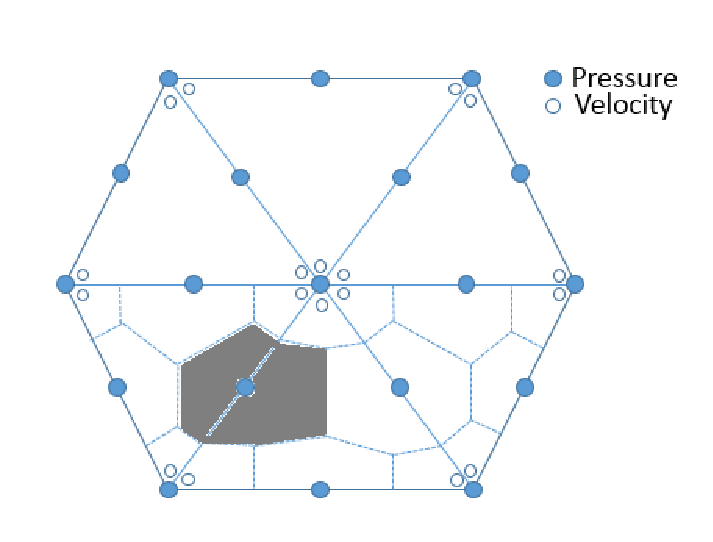
\includegraphics[width=.5\textwidth]{./Pics/P1DGP2.pdf}}
\caption{2D representation of \PN[1]{2} element pairs used in this work. Shaded areas denote control volumes across two contiguous elements. Blue and white circles represent pressure and velocity nodes, respectively.} 
\label{fig:fem_cv}
\end{figure}

\clearpage

%%%%
%%%%  FIGURE
%%%%
\begin{figure}[h]
\centering
\vbox{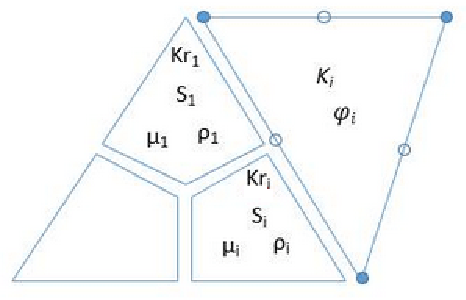
\includegraphics[width=.75\textwidth]{./Pics/element_n.pdf}}
\caption{This is a graphical representation of two different element types. Triangle {\it A} is a representation of the \PN[1]{2} element-pair, whereas triangle {\it B} represents the \PN[1]{1} element-pair. Porosity $\phi_{i}$, permeability {\bf K}$_{i}$, velocity and pressure are primarily represented in FE space whereas scalar fields (such as saturation, density, viscosity etc) are represented in CV space.}
\label{fig:fem_elem}
\end{figure}
\clearpage

%%%%
%%%%  FIGURE 
%%%%
\begin{figure}[h]
\centering
\vbox{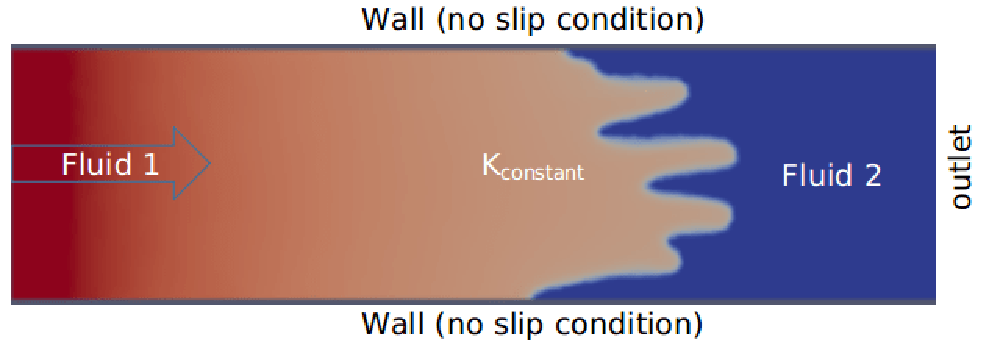
\includegraphics[width=0.75\textwidth]{./Pics/phase_vol_frac_uni_perm_1.pdf}}
\caption{Schematics of formation of flow instabilities during injection of a pure low viscosity fluid (red) into a domain saturated with a second fluid (dark blue). The ratio of viscosity between the two fluids is 5. In this case, the initially piston shape front collapses leading to the formation of several fingers.}
\label{fig:simple_case}
\end{figure}
\clearpage


%%%%
%%%%  FIGURE 
%%%%
\begin{figure}[ht] 
\vbox{
\hbox{\hspace{-0.3cm}
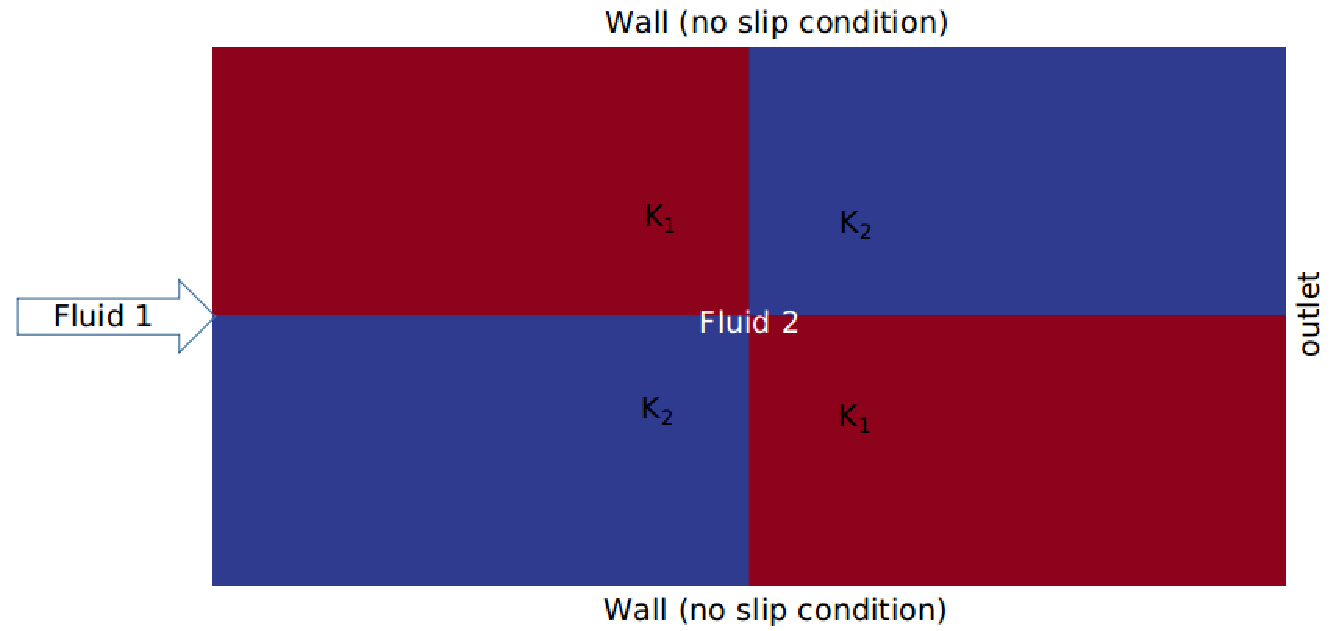
\includegraphics[width=.8\textwidth]{./Pics1/2b2_wi_fine/2b2_whole_in_fine_perm_1.pdf} 
}
\vspace{0.0cm}
\hbox{\hspace{3.5cm} (a) map of permeabilities ($\mathbf{K}$)
}
\vspace{0.25cm}
\hbox{\hspace{1.5cm}
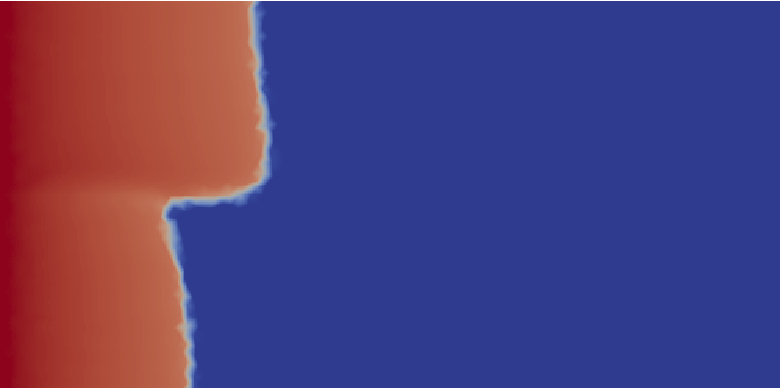
\includegraphics[width=.85\textwidth]{./Pics1/2b2_wi_fine/2b2_whole_in_fine_250_2.pdf}
}
\vspace{0.0cm}
\hbox{\hspace{4.5cm} (b) flow at t=250 
}
\vspace{0.25cm}
\hbox{\hspace{1.5cm}
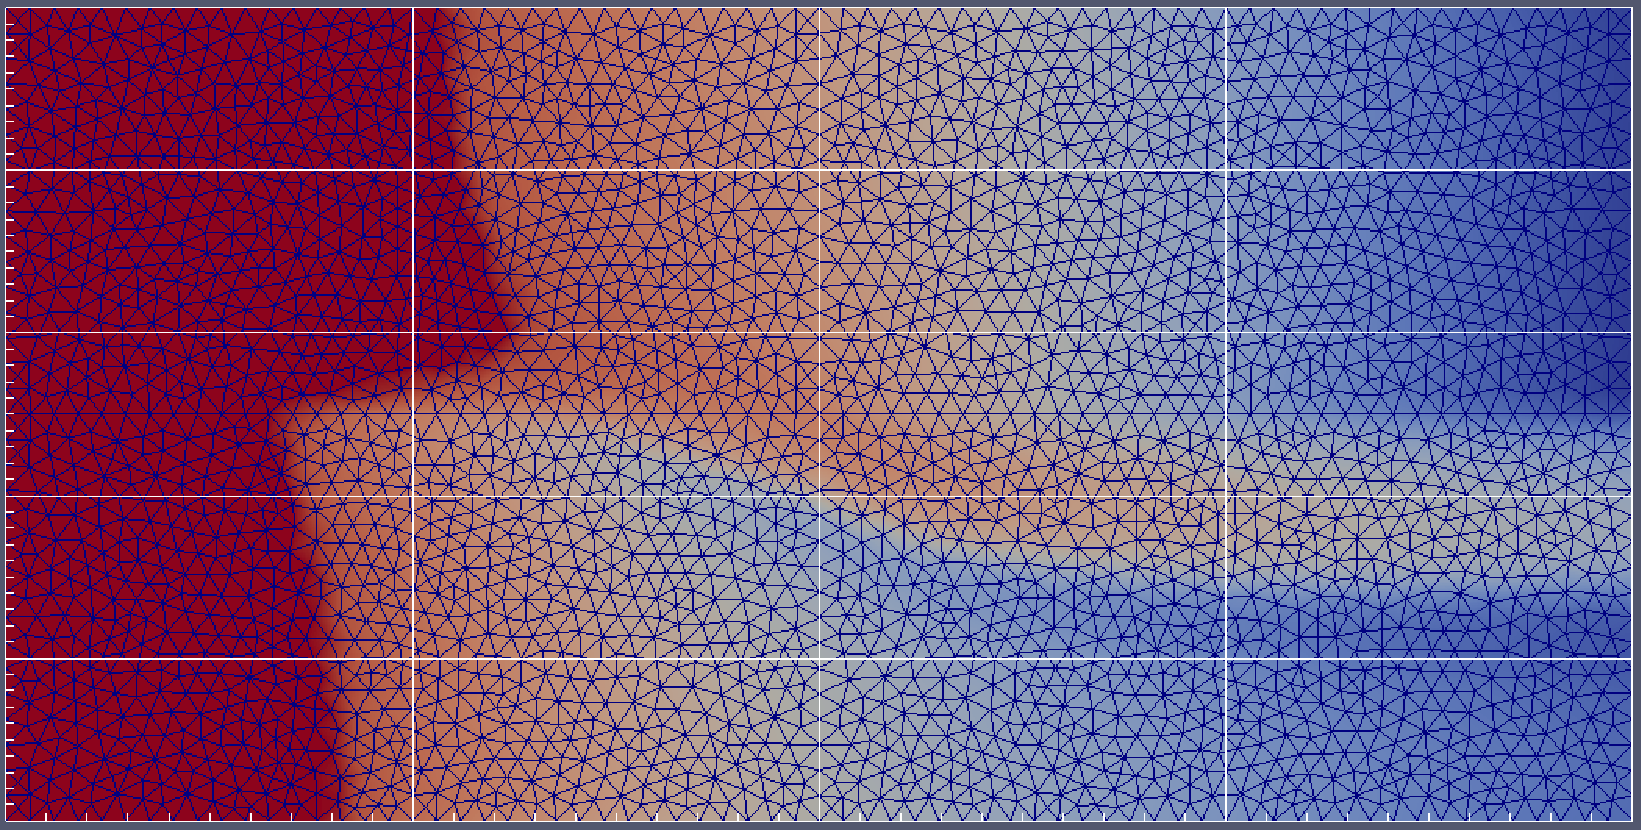
\includegraphics[width=.65\textwidth]{./Pics1/2b2_wi_fine/2b2_whole_in_fine_3000_2.pdf}
}
\vspace{0.0cm}
\hbox{\hspace{4.0cm} (c) flow at t=3000   
}}     
\caption{Model validation of fluid displacement in heterogeneous porous media ({\it VR}=1): (a) the domain is divided into four subdomains with prescribed synthetic permeability, $\mathbf{K}_{1}=1$ and $\mathbf{K}_{2}=2.5$; (b-c) snapshots of saturation (displacing fluid) field at t=$25$s and t=$300$ sec. The domain is discretised with $5960$ \PN[1]{2} elements. }
\label{fem_cv_represent_a}
\end{figure}
\clearpage



%%%%
%%%%  FIGURE
%%%%
\begin{landscape}
\begin{figure}[ht] 
\vbox{\vspace{-1cm}
\hbox{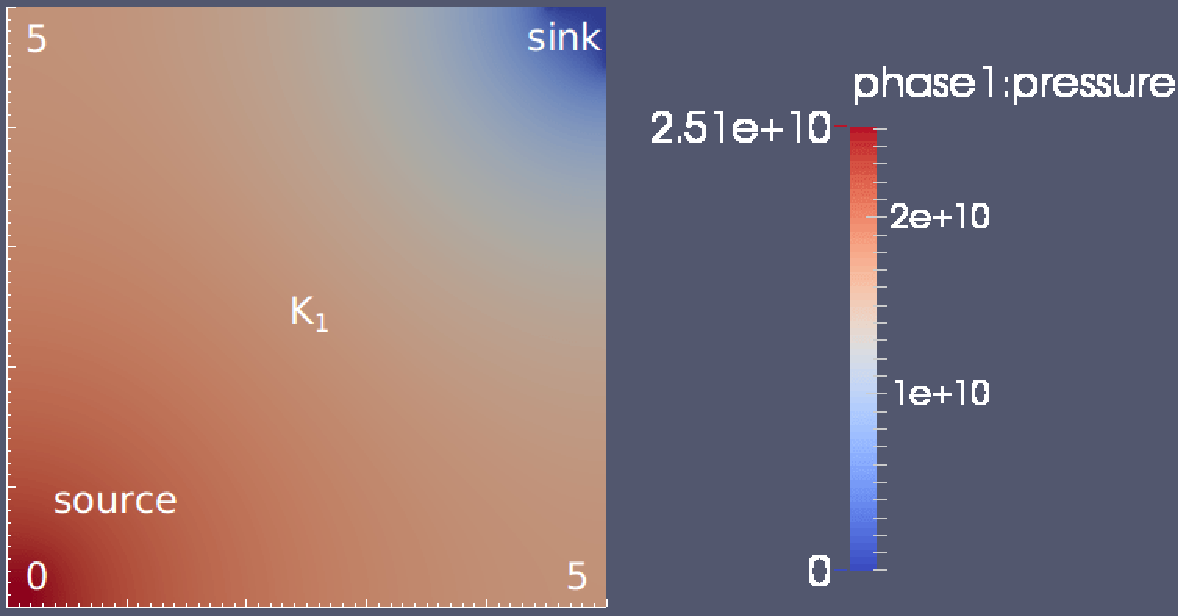
\includegraphics[width=.7\textwidth]{./Pics1/Saffman_homogeneous_MR3/saffman_homo_fixed_2.pdf}
      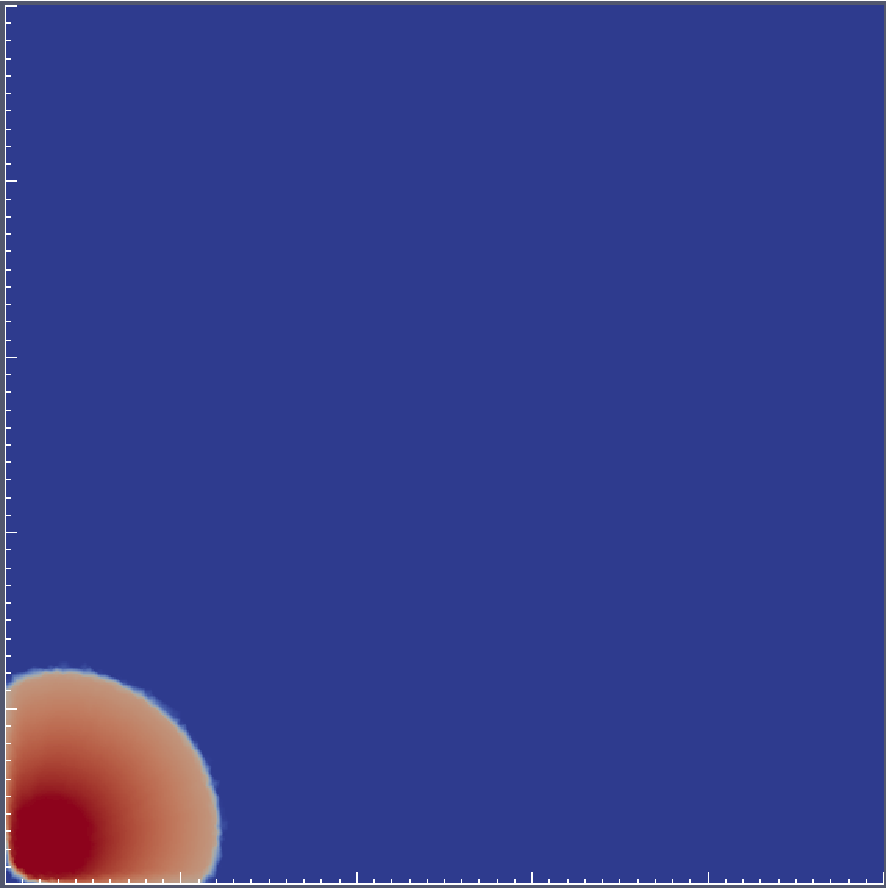
\includegraphics[width=.37\textwidth]{./Pics1/Saffman_homogeneous_MR3/saffman_homo_fixed_250.pdf}
      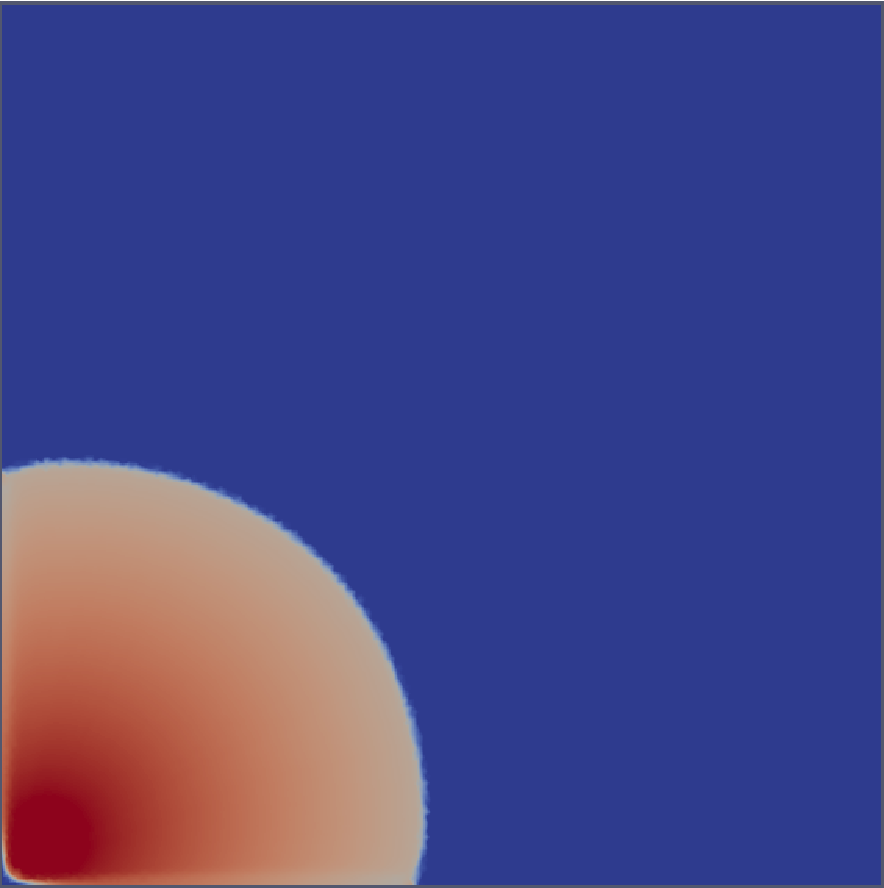
\includegraphics[width=.37\textwidth]{./Pics1/Saffman_homogeneous_MR3/saffman_homo_fixed_1000.pdf}}
\vspace{0.cm}
\hbox{\hspace{2.5cm} (a) pressure at t=0s \hspace{5.cm} (b) t=0.87s \hspace{2.75cm} (c) t=3.54s}
\vspace{0.5cm}
\hbox{
      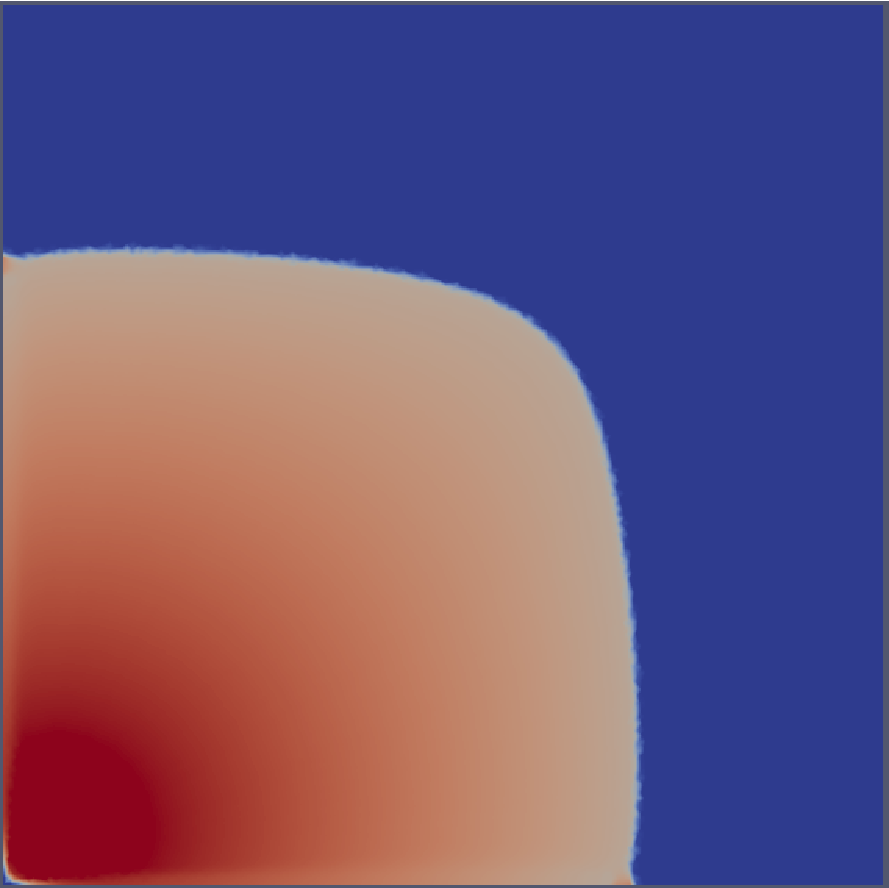
\includegraphics[width=.375\textwidth]{./Pics1/Saffman_homogeneous_MR3/saffman_homo_fixed_2500.pdf}
      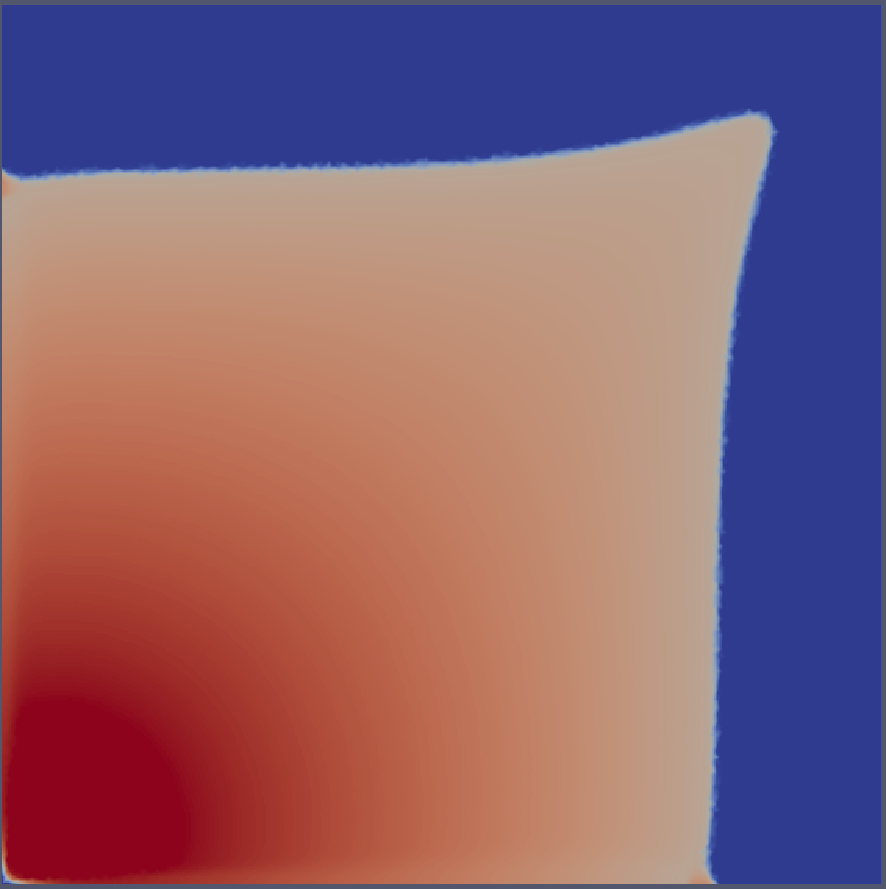
\includegraphics[width=.375\textwidth]{./Pics1/Saffman_homogeneous_MR3/saffman_homo_fixed_3500.pdf} 
      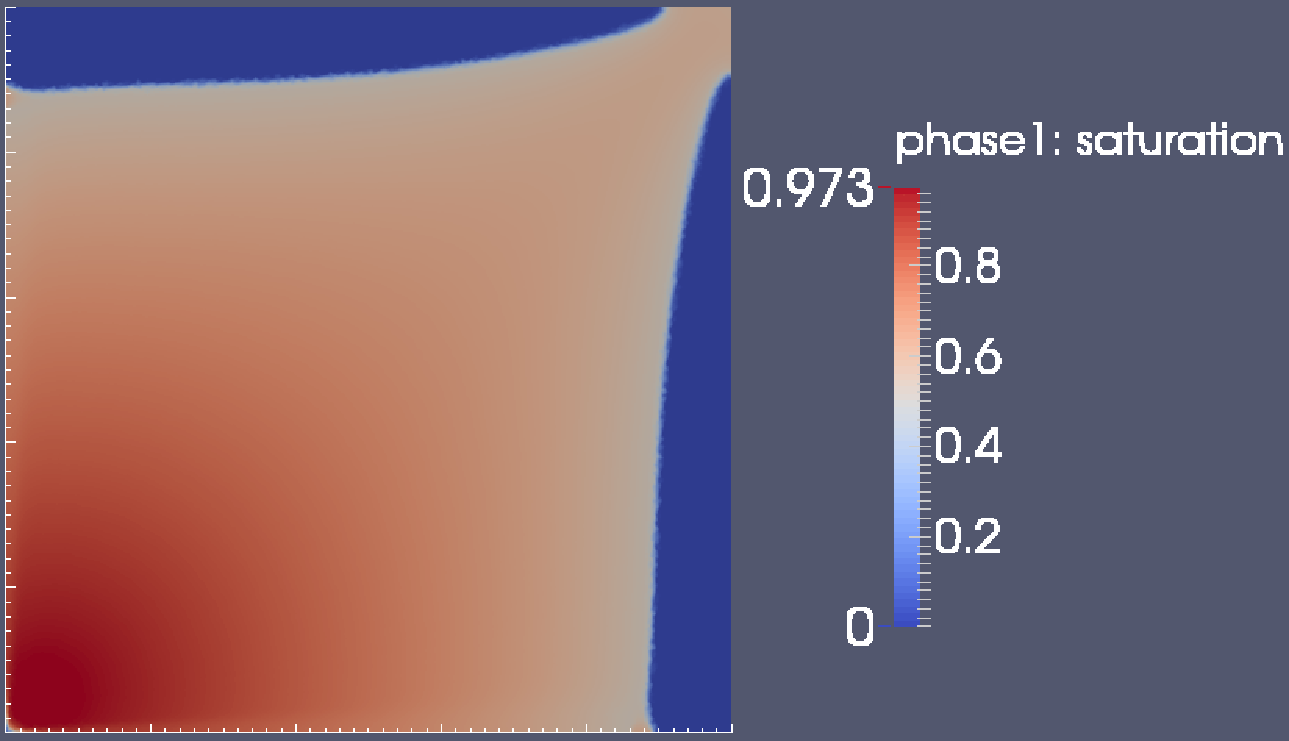
\includegraphics[width=.65\textwidth]{./Pics1/Saffman_homogeneous_MR3/saffman_homo_fixed_end.pdf}}
\vspace{0.cm}
\hbox{ \hspace{1.cm} (d) t=8.86s \hspace{3.0cm} (e) t=12.41s   \hspace{4.0cm} (f) t=17.95s}
\vspace{0.cm}
}   
\caption{Simulated flow in a Hele-Shaw cell ({\it VR}=3): (a) initial pressure profile $\left(\text{in g.cm}^{-1}\text{.s}^{-2}\right)$ with source and sink regions are explicitly shown along with dimensions (in cm); (b-f) snapshots of wetting phase saturation showing flow profile as the simulation evolves. The domain contains $47500$ \PN[1]{2} triangular elements.}
\label{fig:homoheleshaw_VN3}
\end{figure}
\end{landscape}
\clearpage



%%%%
%%%%  FIGURE
%%%%
\begin{landscape}
\begin{figure}[ht] 
\vbox{\vspace{-1cm}
\hbox{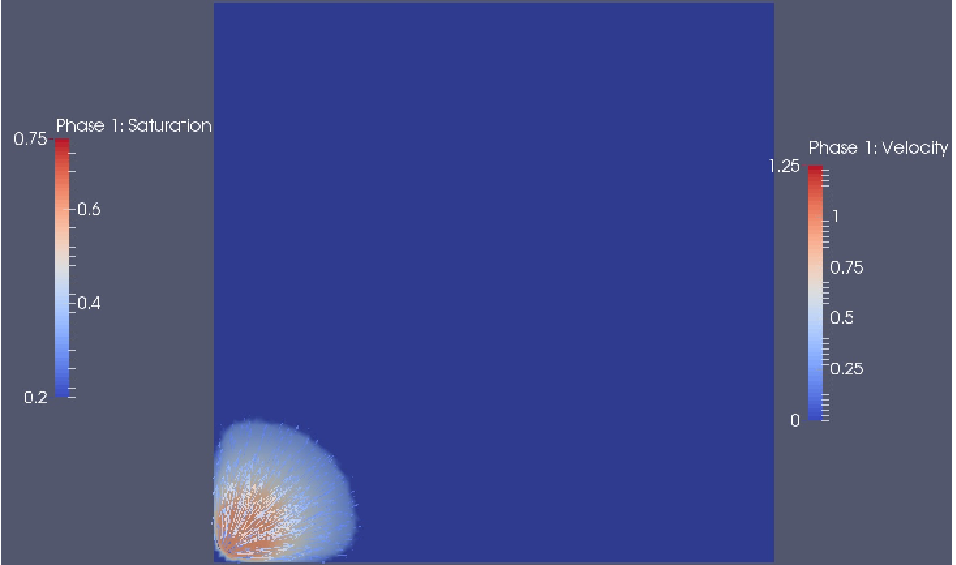
\includegraphics[width=.9\textwidth, height=0.5\textwidth]{./Pics1/Saffman_homogeneous_VR10/ST_Homog_VR10_D201c.pdf}
\hspace{0.5cm}      
      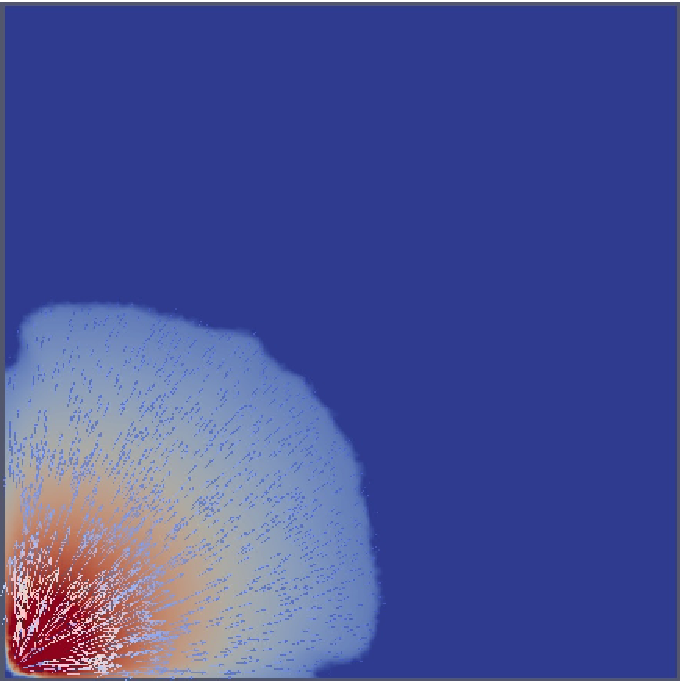
\includegraphics[width=.5\textwidth]{./Pics1/Saffman_homogeneous_VR10/ST_Homog_VR10_D1001c.pdf}}
\vspace{0.cm}
\hbox{\hspace{5.cm} (a) t=0.66s \hspace{8.cm} (b) t=3.43s }
\vspace{0.5cm}
\hbox{
      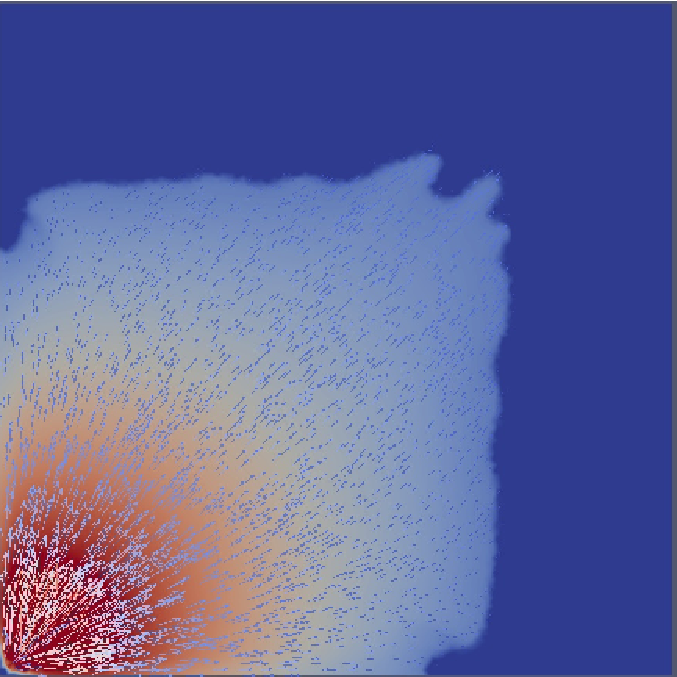
\includegraphics[width=.5\textwidth]{./Pics1/Saffman_homogeneous_VR10/ST_Homog_VR10_D2001c}
      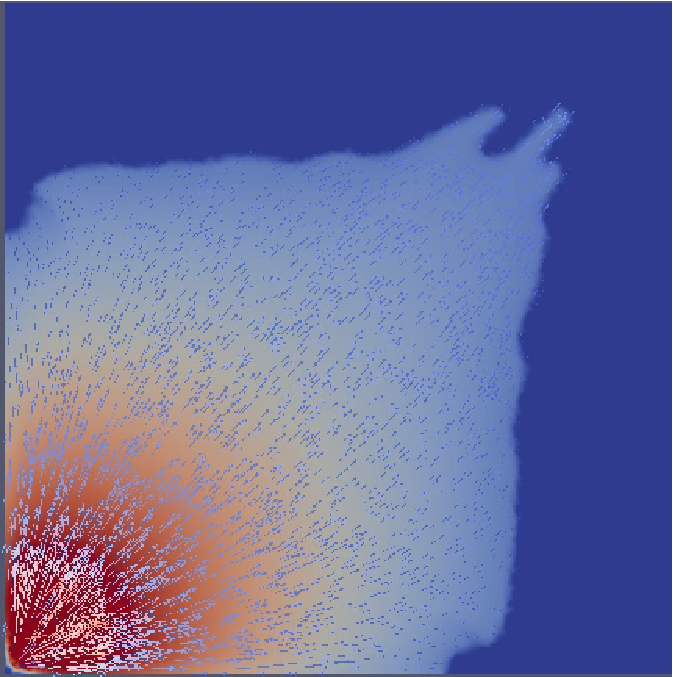
\includegraphics[width=.5\textwidth]{./Pics1/Saffman_homogeneous_VR10/ST_Homog_VR10_D2201c}
      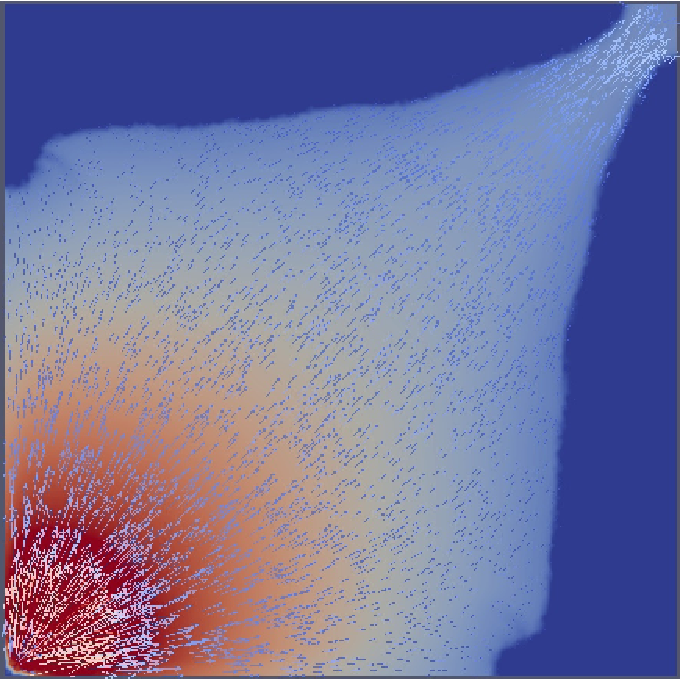
\includegraphics[width=.5\textwidth]{./Pics1/Saffman_homogeneous_VR10/ST_Homog_VR10_D3001c}}
\vspace{0.cm}
\hbox{ \hspace{2.cm} (c) t=6.92s \hspace{4.5cm} (d) t=7.61s \hspace{4.5cm} (e)t=10.00s}
\vspace{0.cm}
}   
\caption{Simulated flow in a Hele-Shaw cell ({\it VR}=10): snapshots of overlapped wetting phase saturation and velocity vectors showing flow profile as the simulation evolves. The domain contains $26313$ \PN[1]{2} triangular elements.}
\label{fig:homoheleshaw_VN10}
\end{figure}
\end{landscape}
\clearpage

%%%%
%%%%  FIGURE
%%%%
\begin{landscape}
\begin{figure}[ht] 
\vbox{\vspace{-1cm}
\hbox{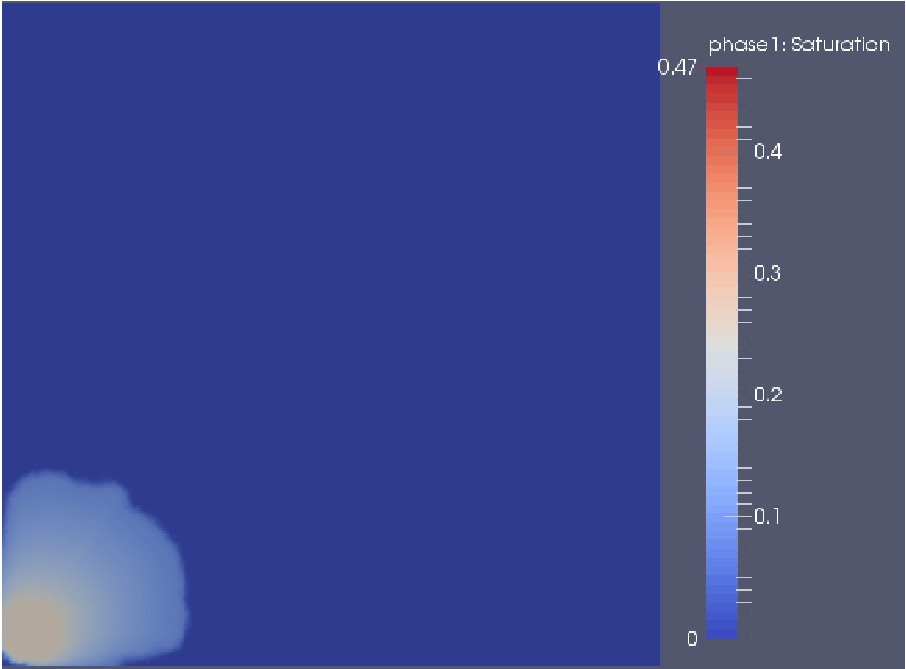
\includegraphics[width=.9\textwidth, height=0.5\textwidth]{./Pics1/Saffman_homogeneous_VR150/ST_Homog_VR150_D300b}
\hspace{0.5cm}      
      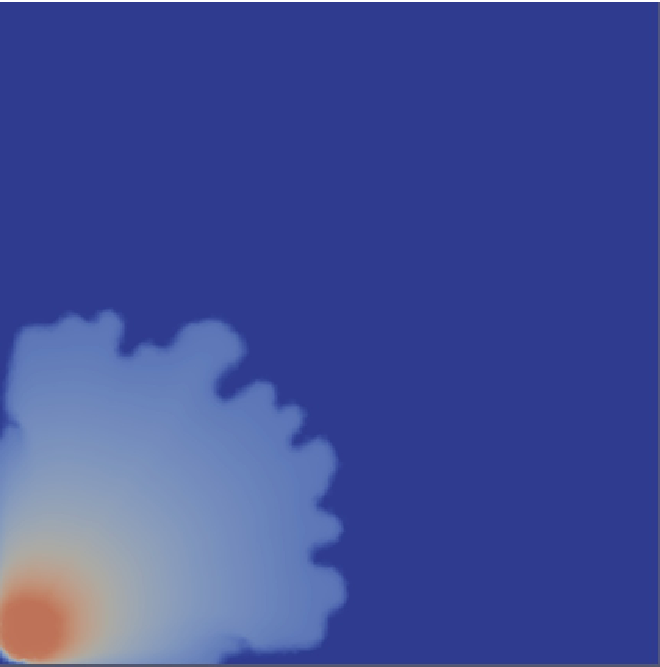
\includegraphics[width=.5\textwidth]{./Pics1/Saffman_homogeneous_VR150/ST_Homog_VR150_D1600b}}
\vspace{0.cm}
\hbox{\hspace{5.cm} (a) t=0.27s \hspace{8.cm} (b) t=0.94s }
\vspace{0.5cm}
\hbox{
      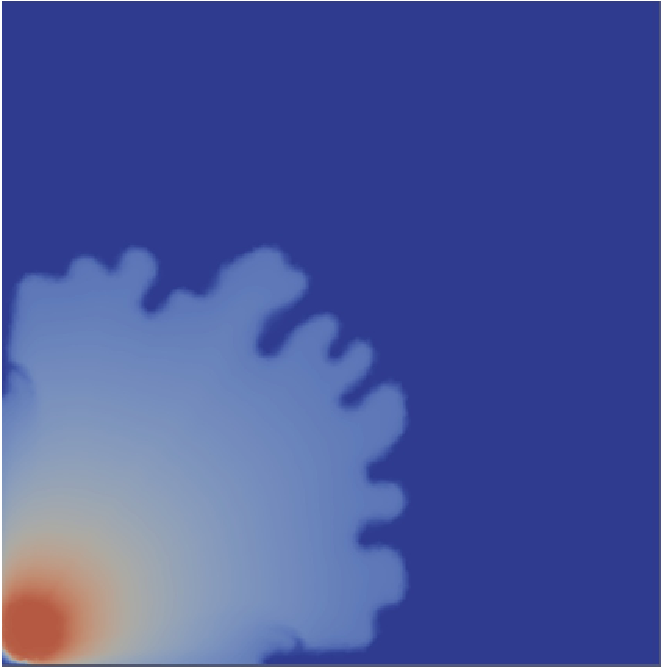
\includegraphics[width=.5\textwidth]{./Pics1/Saffman_homogeneous_VR150/ST_Homog_VR150_D2700b}
      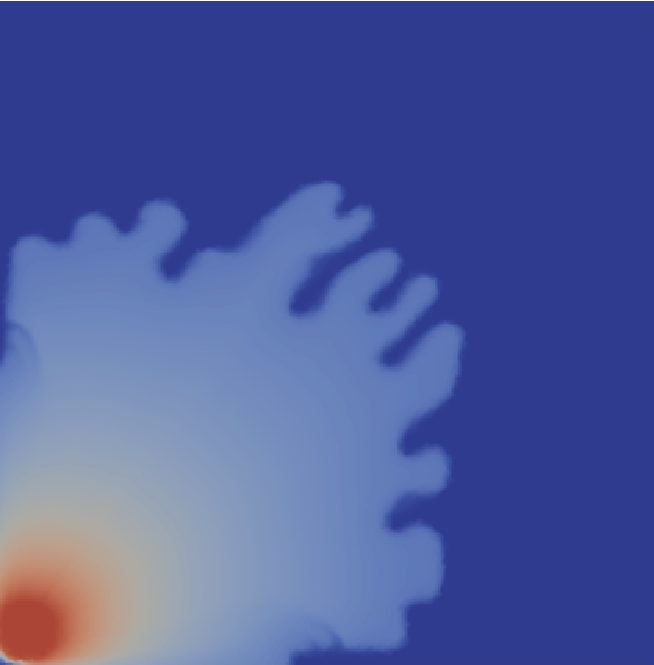
\includegraphics[width=.5\textwidth]{./Pics1/Saffman_homogeneous_VR150/ST_Homog_VR150_D4000b}
      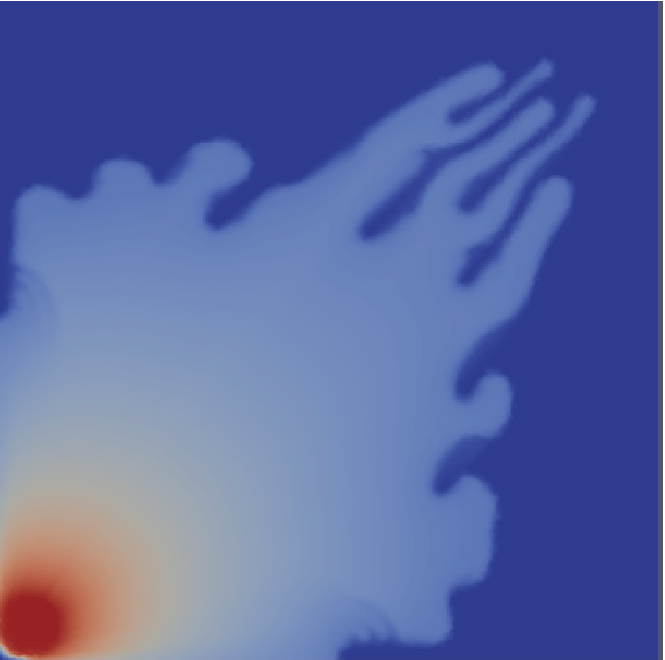
\includegraphics[width=.5\textwidth]{./Pics1/Saffman_homogeneous_VR150/ST_Homog_VR150_D7000b}}
\vspace{0.cm}
\hbox{ \hspace{2.cm} (c) t=1.32s \hspace{4.5cm} (d) t=1.70s \hspace{4.5cm} (e)t=2.31s}
\vspace{0.cm}
}   
\caption{Simulated flow in a Hele-Shaw cell ({\it VR}=150): snapshots of wetting phase saturation showing flow profile as the simulation evolves. The domain contains $26313$ \PN[1]{2} triangular elements.}
\label{fig:homoheleshaw_VN10}
\end{figure}
\end{landscape}
\clearpage


%%%%
%%%%  FIGURE
%%%%
\begin{landscape}
\begin{figure}[ht] 
\hbox{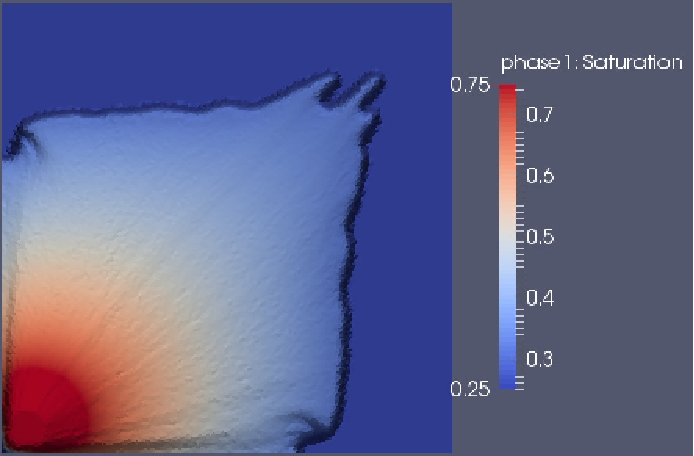
\includegraphics[width=.5\textwidth]{./Pics1/Saffman_homogeneous_VR10/ST_Homog_VR10_D2201_bbd}
       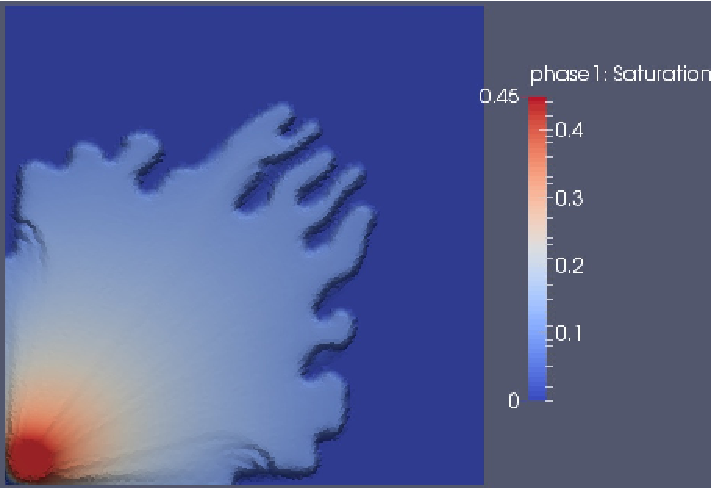
\includegraphics[width=.49\textwidth]{./Pics1/Saffman_homogeneous_VR150/ST_Homog_VR150_D5003_k2b}}
\caption{Simulated flow in Hele-Shaw cells performed with viscosity ratios of 10 (left, t=7.61s) and 150 (t=1.94s). Width of largest fingers are approximetely 0.70 and 0.90cm, which are in good agreement with values obtained from \citet{guan_2003}'s analytic solution. Domains of both simulations contain $26313$ \PN[1]{2} triangular elements.\red{(More pics to be added!!)}}
\label{fig:homoheleshaw_VN10_VN150}
\end{figure}
\end{landscape}



\begin{comment}

%%%%
%%%%  FIGURE
%%%%
\begin{landscape}
\begin{figure}[ht] 
\vbox{\vspace{-1cm}
\hbox{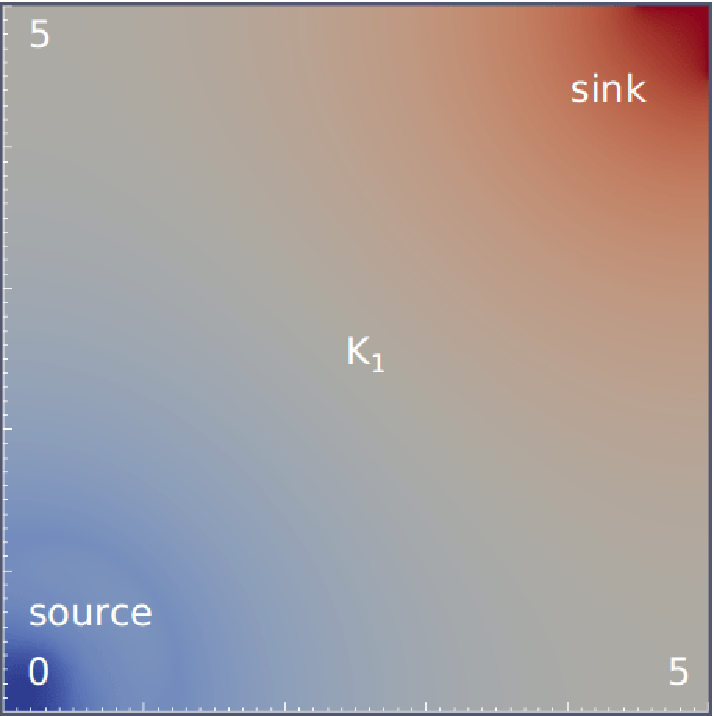
\includegraphics[width=.5\textwidth]{./Pics1/Saffman_homogeneous/saffman_homo_fixed_1.pdf}
      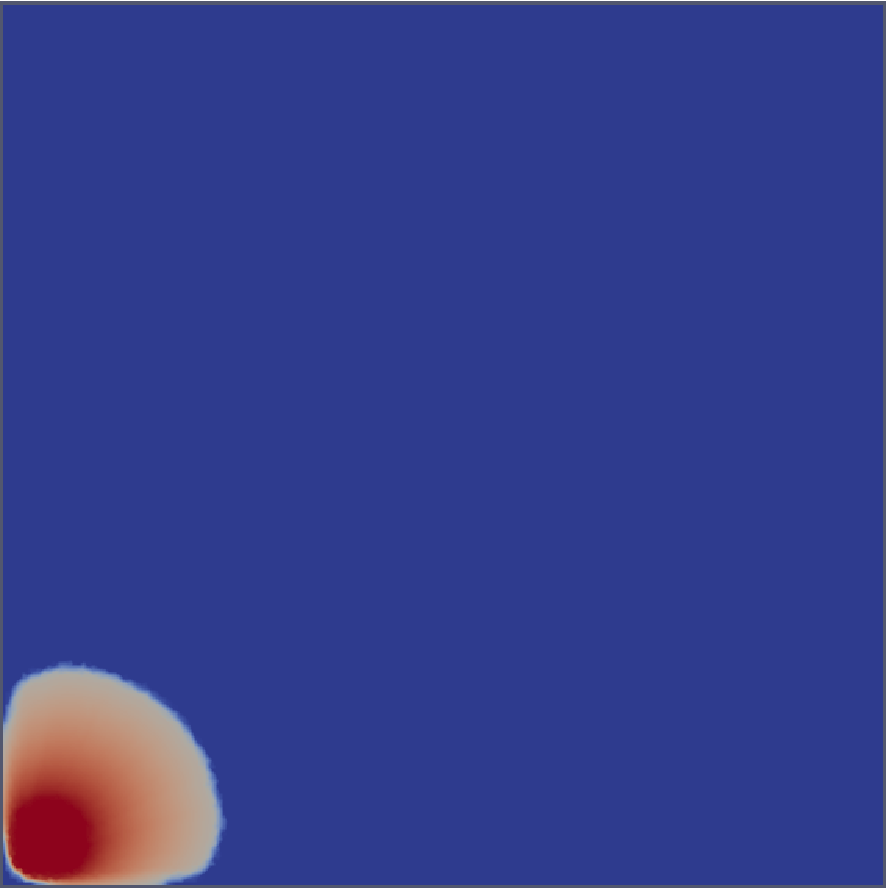
\includegraphics[width=.5\textwidth]{./Pics1/Saffman_homogeneous/saffman_homo_fixed_250_1.pdf}
      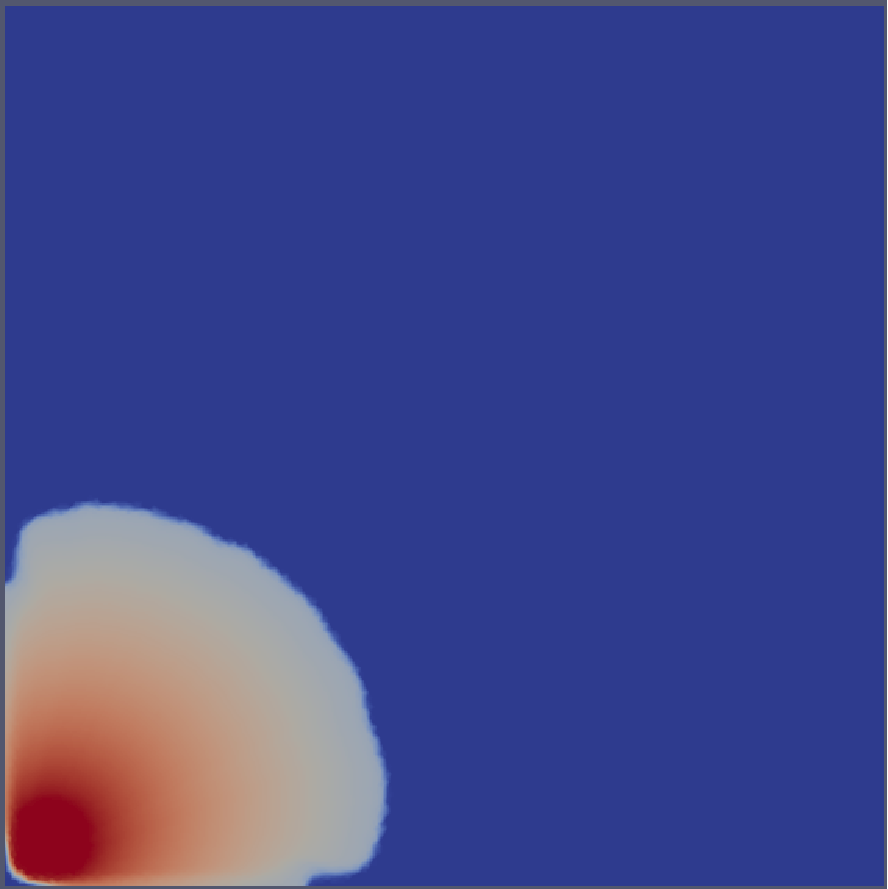
\includegraphics[width=.5\textwidth]{./Pics1/Saffman_homogeneous/saffman_homo_fixed_1000.pdf}}
\vspace{0.cm}
\hbox{\hspace{1.0cm} (a) pressure at t=0 \hspace{3.cm} (b) t=250\red{(???)} \hspace{3.0cm} (c) t=1000\red{(???)}}
\vspace{0.5cm}
\hbox{
      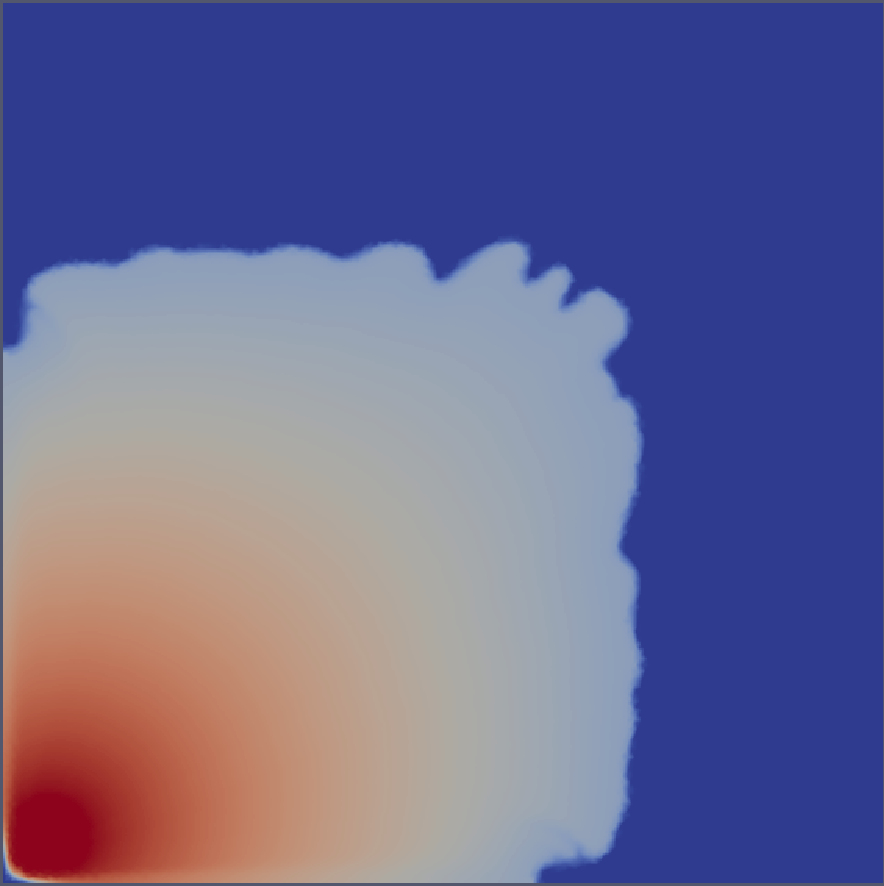
\includegraphics[width=.5\textwidth]{./Pics1/Saffman_homogeneous/saffman_homo_fixed_6000.pdf}
      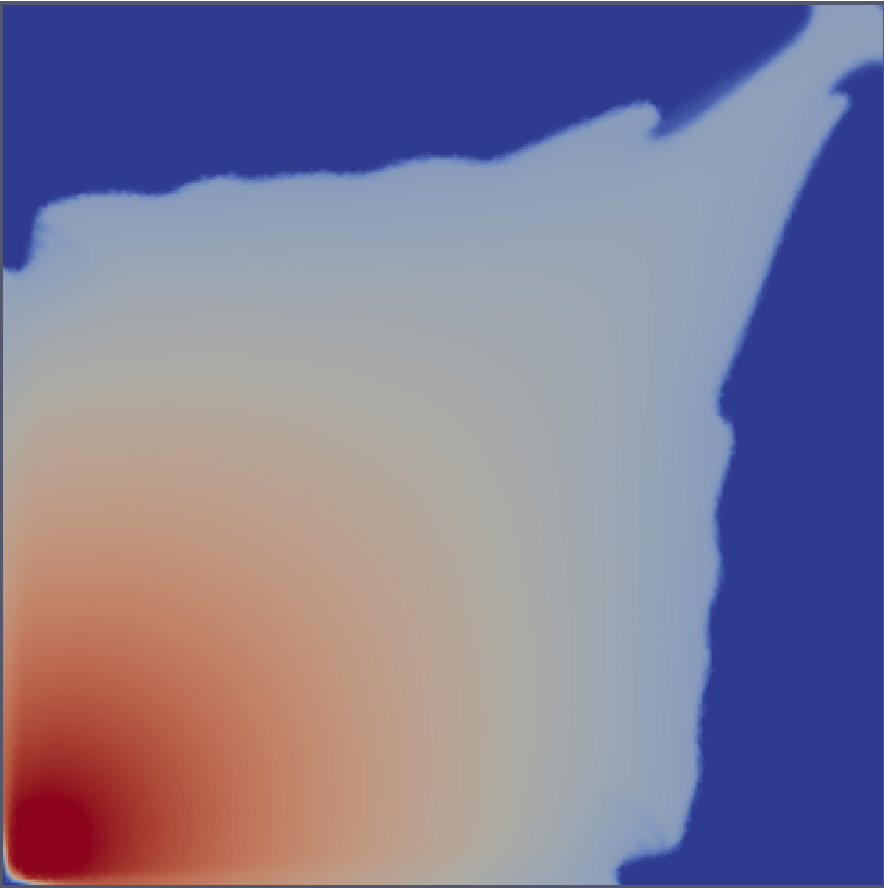
\includegraphics[width=.5\textwidth]{./Pics1/Saffman_homogeneous/saffman_homo_fixed_end_1.pdf}}
\vspace{0.cm}
\hbox{ \hspace{2.cm} (d) t=6000\red{(???)} \hspace{3.cm} (e) t=XXX\red{(???)}}
\vspace{0.cm}
}   
\caption{Simulated flow in a Hele-Shaw cell ({\it VR}=10): (a) pressure profile $\left(\text{in g.cm}^{-1}\text{.s}^{-2}\right)$ with source and sink regions explicitly shown along with dimensions (in cm); (b-e) snapshots of wetting phase saturation showing flow profile as the simulation evolves. The domain contains $47000$ \PN[1]{2} triangular elements. The pressure and saturation range of values are the same like the  case in fig.\ref{fig:homoheleshaw_VN3}.}
\label{fig:homoheleshaw_VN10}
\end{figure}
\end{landscape}
\clearpage
\end{comment}


%%%
%%% FIGURE XXXXXX
%%%
\begin{landscape}
  \begin{figure}[ht]
  \vbox{\vspace{-1cm}
      \hbox{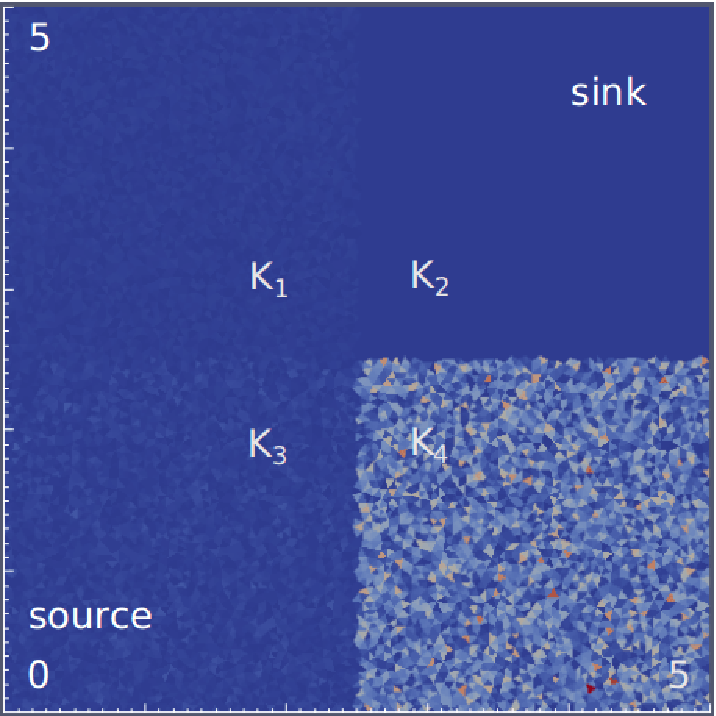
\includegraphics[width=.5\textwidth]{./Pics1/Saffman_heterogeneous/saffman_heter_fixed_1.pdf}
            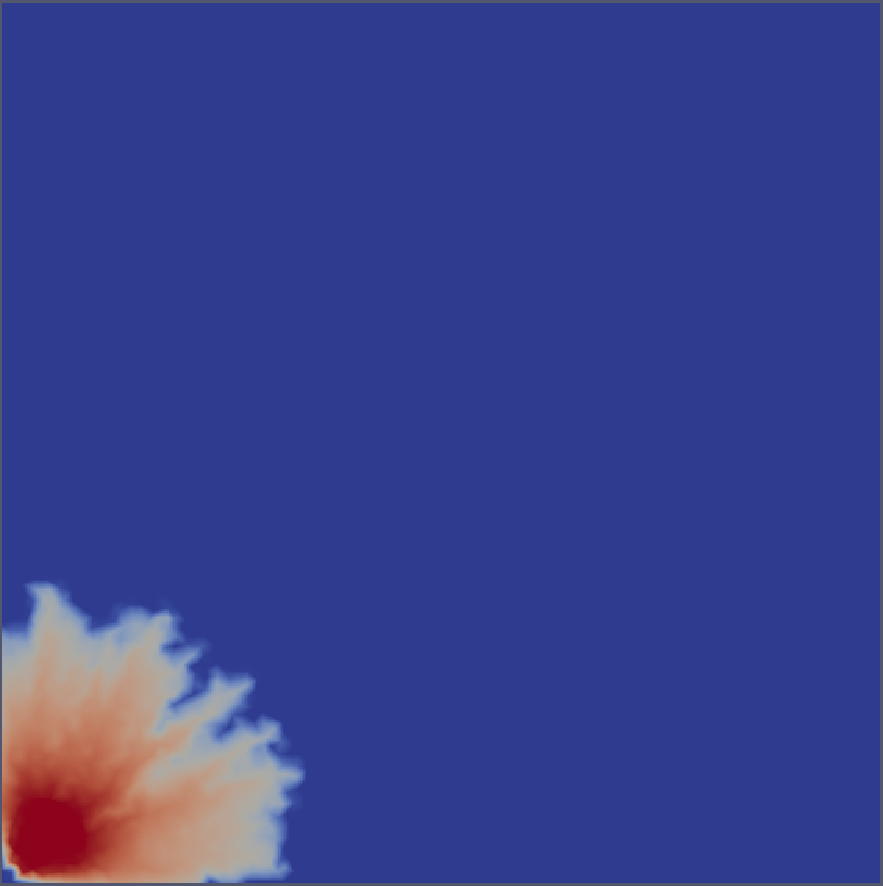
\includegraphics[width=.5\textwidth]{./Pics1/Saffman_heterogeneous/saffman_heter_fixed_500.pdf} 
            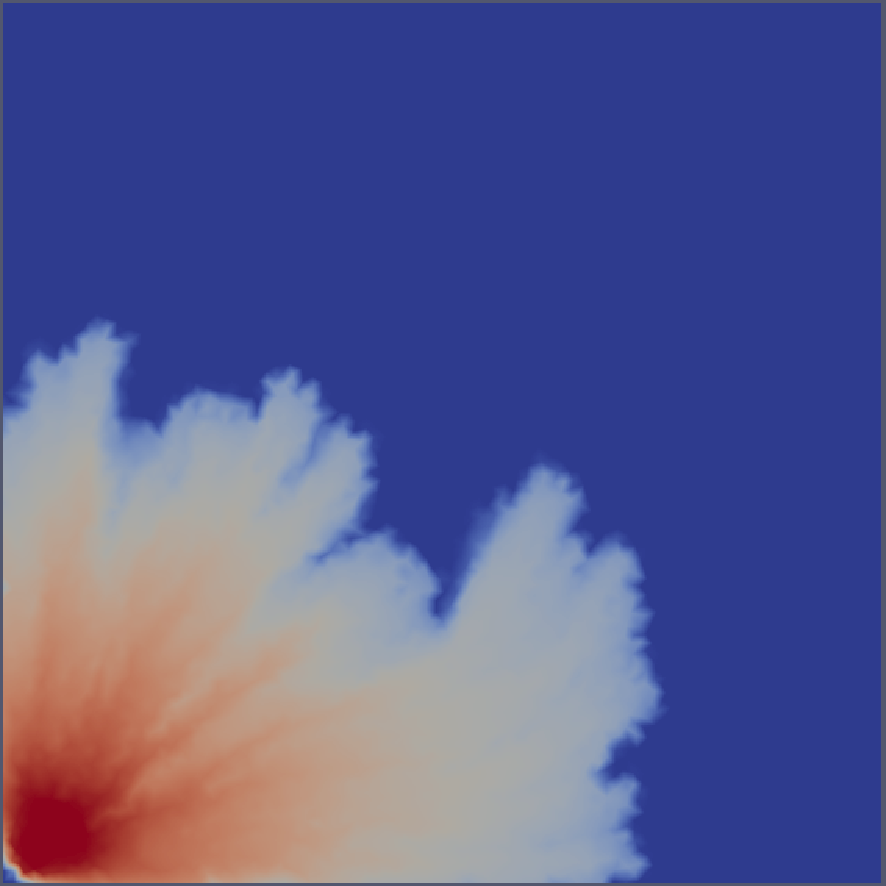
\includegraphics[width=.5\textwidth]{./Pics1/Saffman_heterogeneous/saffman_heter_fixed_2000.pdf} }
      \hbox{\hspace{1.0cm} (a) permeability map \hspace{3.cm} (b) t=0.75s \hspace{4.0cm} (c) t=8s}
      \vspace{0.5cm}
      \hbox{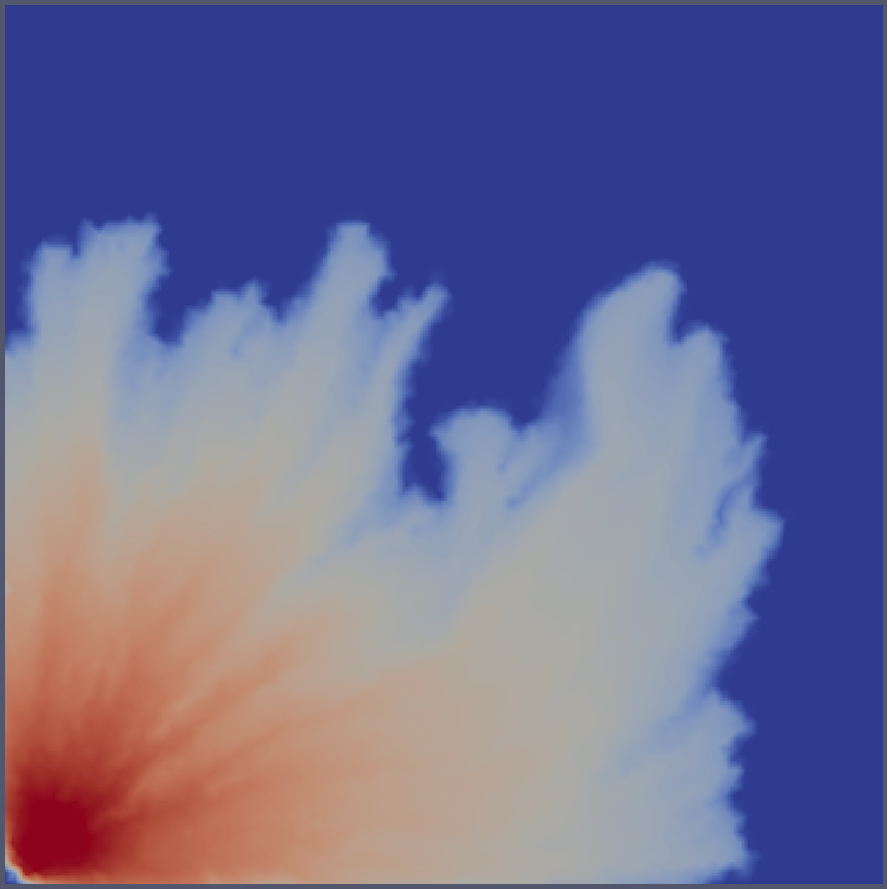
\includegraphics[width=.5\textwidth]{./Pics1/Saffman_heterogeneous/saffman_heter_fixed_3000.pdf}
            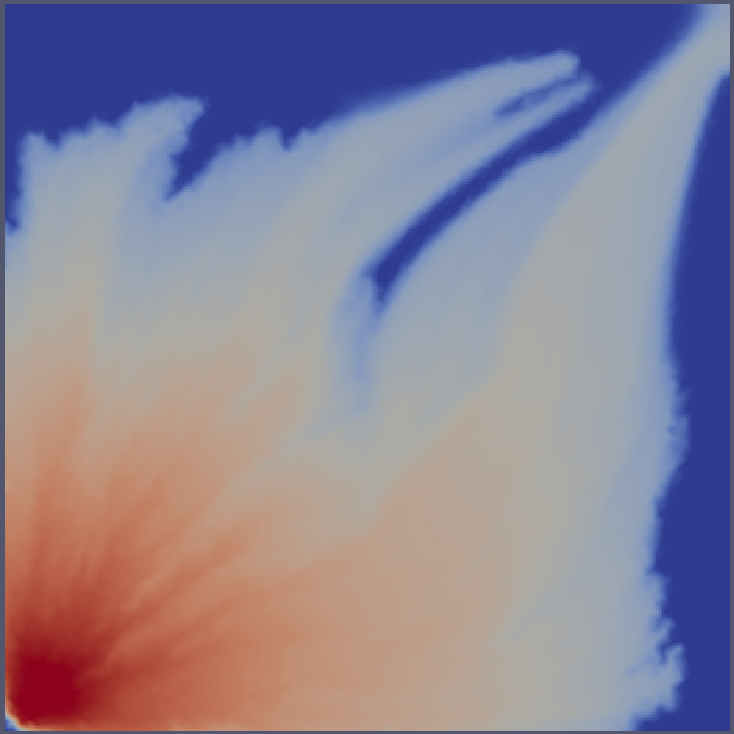
\includegraphics[width=.5\textwidth]{./Pics1/Saffman_heterogeneous/saffman_heter_fixed_6000.pdf}
            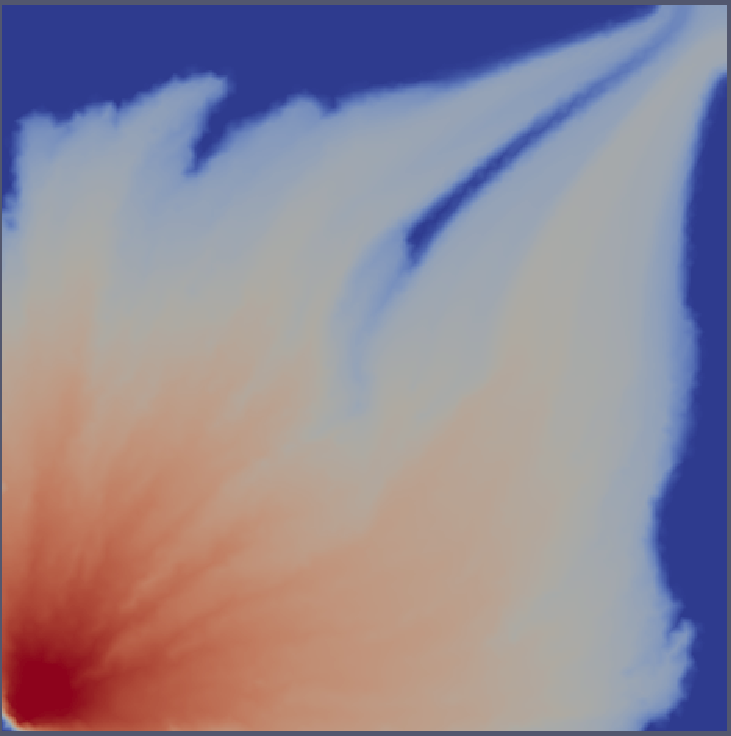
\includegraphics[width=.5\textwidth]{./Pics1/Saffman_heterogeneous/saffman_heter_fixed_24000.pdf} }
      \hbox{\hspace{2.5cm} (d) t=18s \hspace{5.cm} (e) t= \hspace{3.0cm} (f) t=24000 }}
\caption{Simulated flow in a modified Hele-Shaw cell with {\it VR}=10: (a) permeability distribution $\left(\text{10}^{-10}\le\mathbf{K}_{1}\le\text{5}\times\text{10}^{-10}\right.$, {\bf K}$_{2}$=10$^{-10}$, 10$^{-11}\le\mathbf{K}_{3}\le$ 5$\times$10$^{-10}$ and 10$^{-12}\le\mathbf{K}_{4}\le$ 5$\times$10$\left.^{-10}\text{ cm}^{2}\right)$; (b-f) snapshots of saturation profile during \red{XX} seconds of simulation. The domain contains \red{XX} \PN[1]{2} element-pairs.}
\label{fig:HeleShawHeter_VR10}
\end{figure}
\end{landscape}
\clearpage



%%%%
%%%%  FIGURE
%%%%
\begin{landscape}
\begin{figure}[ht] 
\vbox{
\hbox{\hspace{4.0cm}
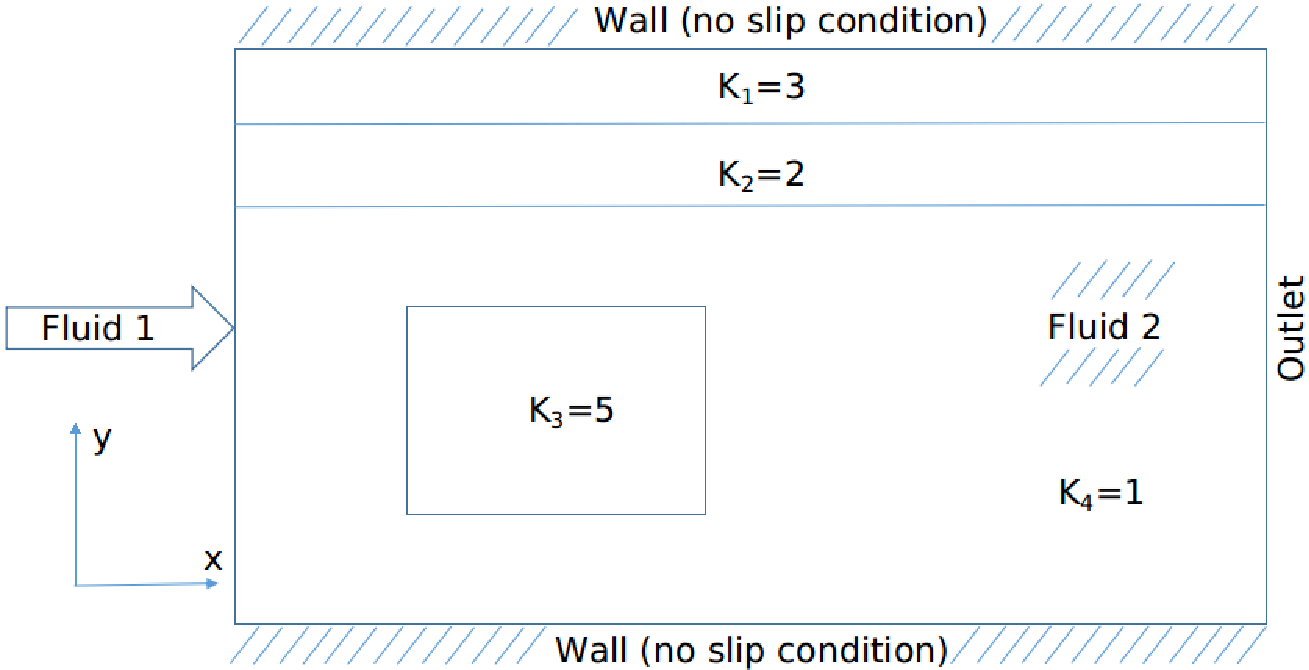
\includegraphics[width=.75\textwidth]{./Pics/map_of_boundaries.pdf} 
}
\vspace{0.0cm}
\hbox{\hspace{6.5cm} (a) map of permeabilties K   
}
\vspace{0.25cm}
\hbox{\hspace{4.0cm}
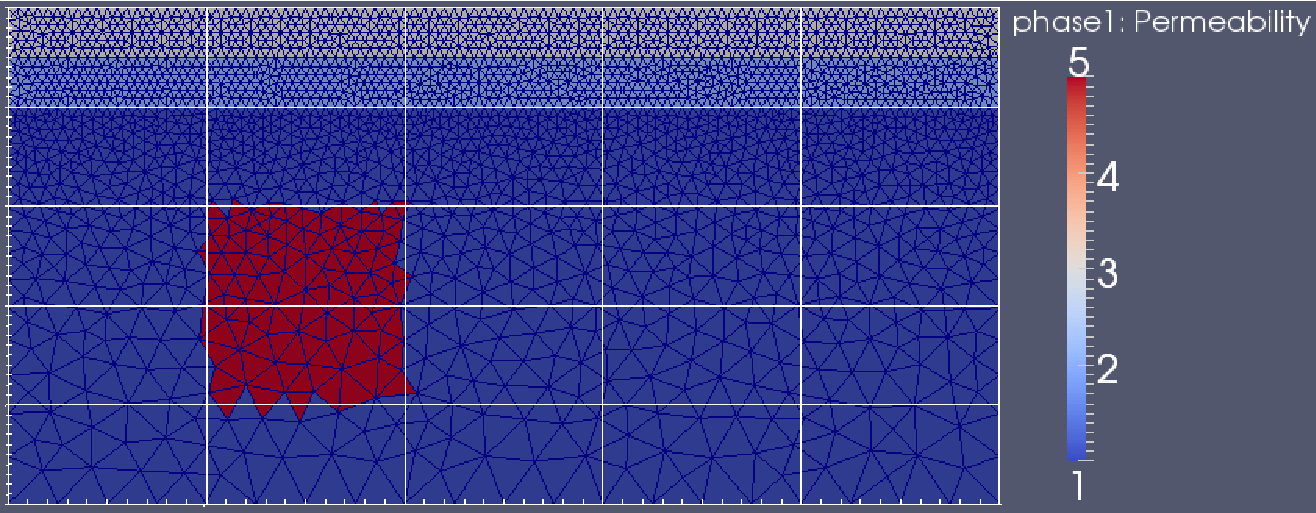
\includegraphics[width=.9\textwidth]{./Pics/map_of_boundaries_1.pdf}
}
\vspace{0.0cm}
\hbox{\hspace{9cm} (b)      
}
}     
\caption{Figure (a) describes the initial and boundary conditions as these are applied in this set of simulations. Below (b) there is a comparison between the unstructured and fixed mesh and the unstructured and adaptive mesh. During the implementation of fixed mesh initially there $4606$ elements while for the adaptive mesh there are $606$ while the majority of them is on the interface between between the two fluids. }
\label{fig:testcase_heter_domain}
\end{figure}
\end{landscape}
\clearpage



%%%%
%%%%  FIGURE
%%%%
\begin{landscape}
\begin{figure}[ht] 
\vbox{
\hbox{\hspace{3.5cm}
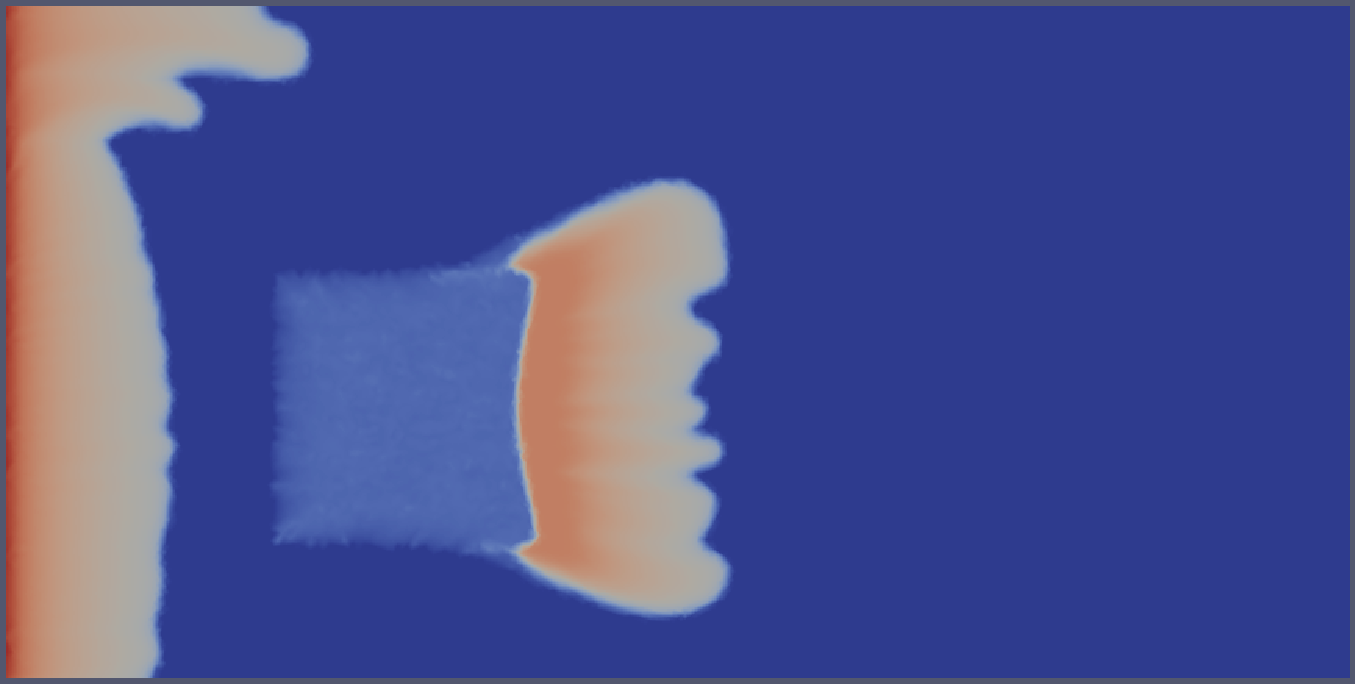
\includegraphics[width=.65\textwidth]{./Pics1/mr10_5regions_fixed/5regions_fixed_250.pdf} 
}
\vspace{0.0cm}
\hbox{\hspace{6.5cm} (a) flow at t=250 (fixed mesh)  
}
\vspace{0.25cm}
\hbox{\hspace{3.5cm}
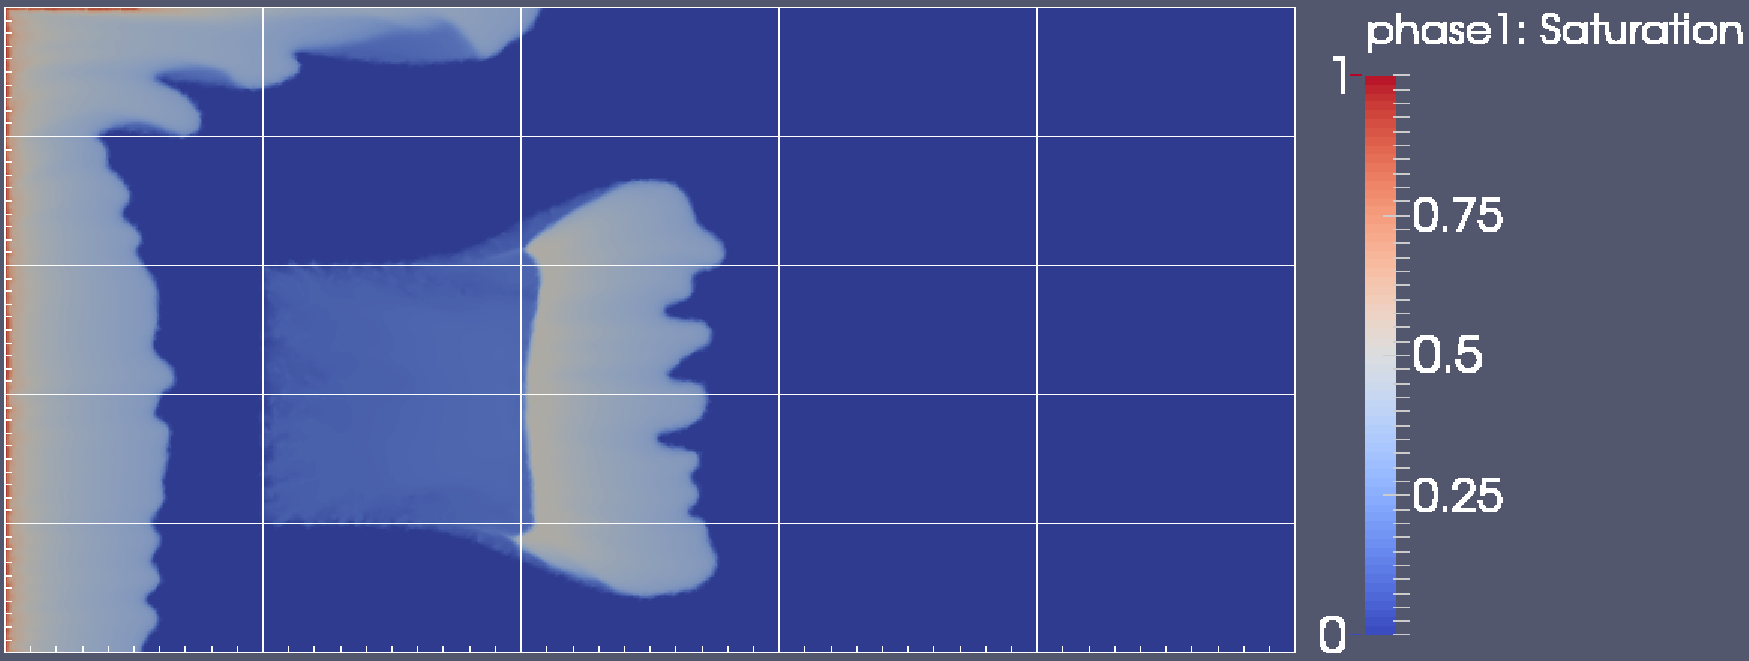
\includegraphics[width=.9\textwidth]{./Pics1/mr10_5regions_adapt/5regions_adapt_250_1.pdf}
}
\vspace{0.0cm}
\hbox{\hspace{6.5cm} (b) flow at t=250 (adaptive mesh)    
}
}     
\caption{For $t=0.125$s, $2$ test-cases under the VR=$10$ and under fixed (top) and adaptive(bottom) mesh are compared. There is a significant difference on the main front (left hand side of the domain) and the number of finger that appear.}
\label{fig:2testcase_a}
\end{figure}
\end{landscape}
\clearpage


%%%%
%%%%  FIGURE
%%%%
\begin{landscape}
\begin{figure}[ht] 
\vbox{
\hbox{\hspace{3.5cm}
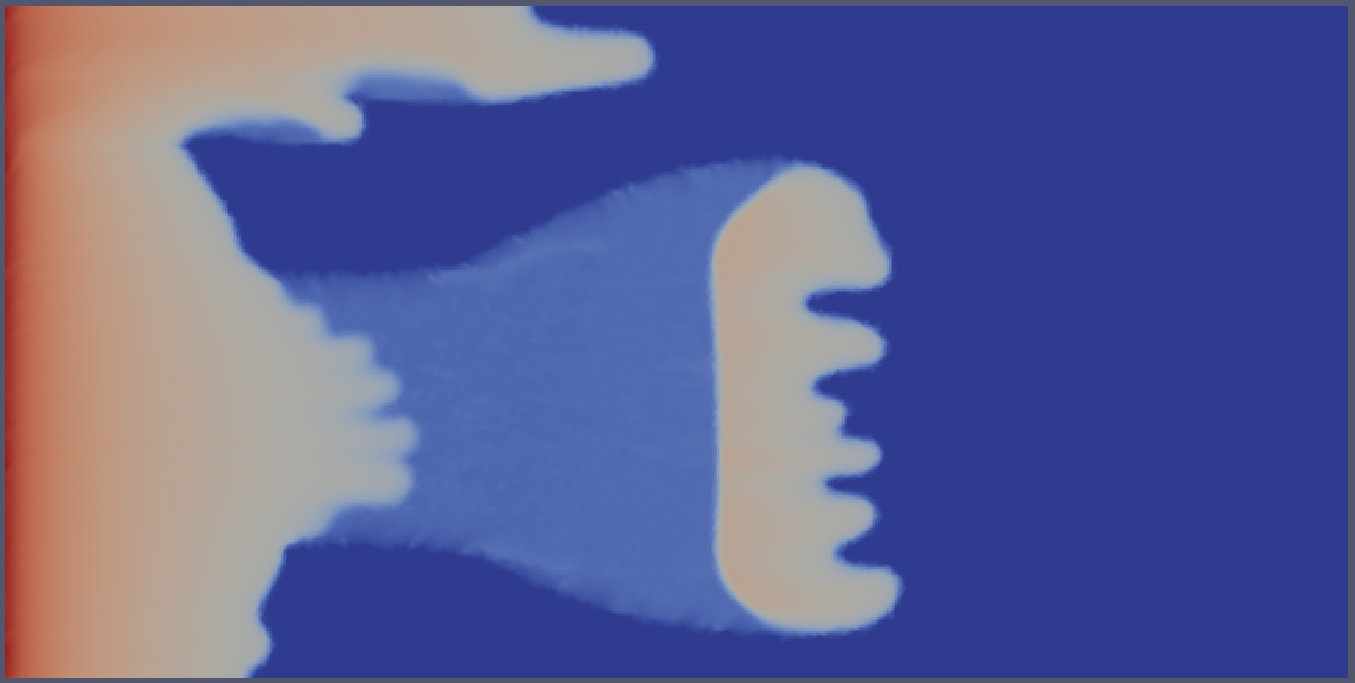
\includegraphics[width=.65\textwidth]{./Pics1/mr10_5regions_fixed/5regions_fixed_500.pdf} 
}
\vspace{0.0cm}
\hbox{\hspace{6.5cm} (a) flow at t=500 (fixed mesh)   
}
\vspace{0.25cm}
\hbox{\hspace{3.5cm}
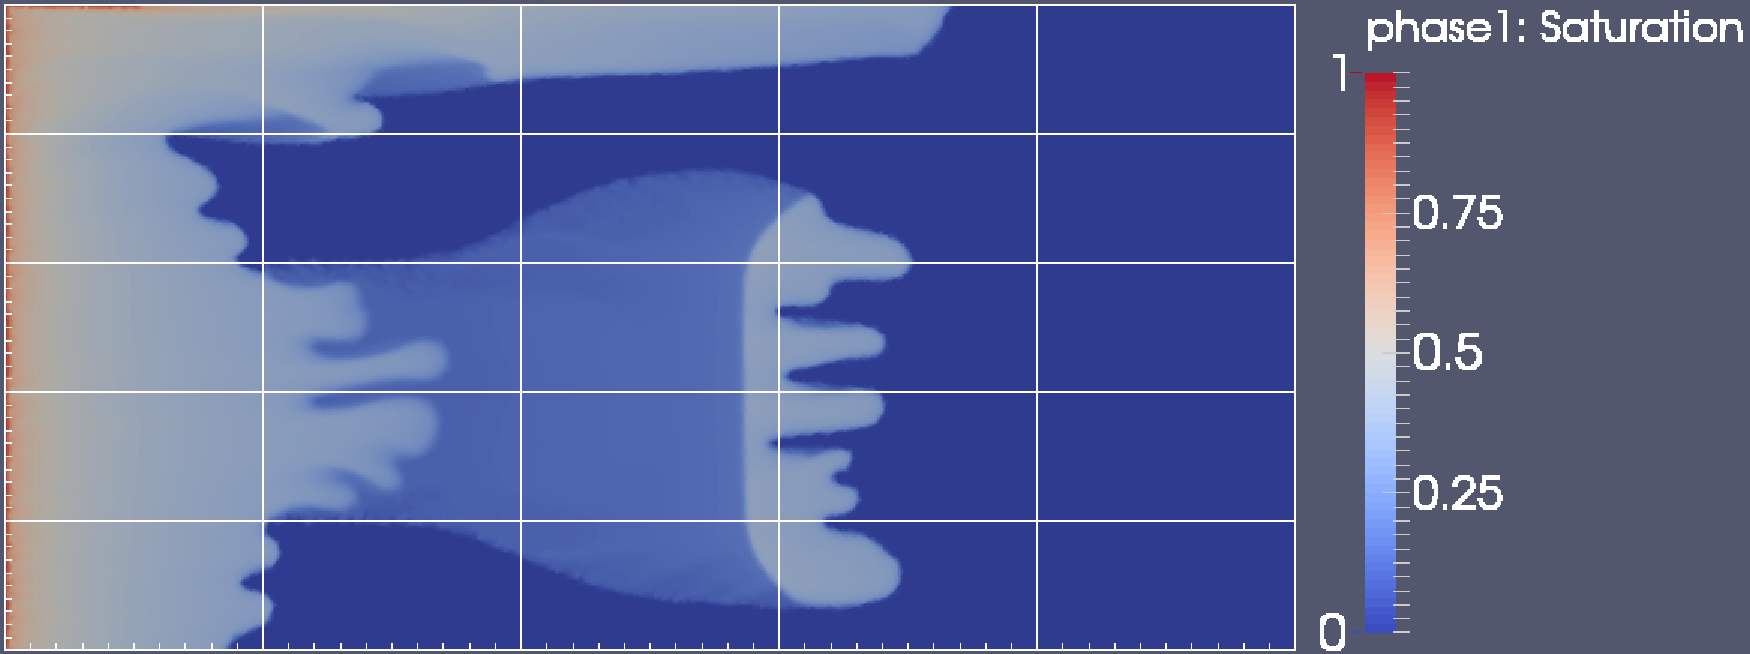
\includegraphics[width=.9\textwidth]{./Pics1/mr10_5regions_adapt/5regions_adapt_500_1.pdf}
}
\vspace{0.0cm}
\hbox{\hspace{6.5cm} (b) flow at t=500 (adaptive mesh)     
}
}     
\caption{At $t=0.25$s ($t=500$, timestemp) cross flow is taking place at the upper part of the formation. The fingers start to becoming more proufound as can been seen at the bottom.}
\label{fig:2testcase_b}
\end{figure}
\end{landscape}
\clearpage



%%%%
%%%%  FIGURE
%%%%
\begin{landscape}
\begin{figure}[ht] 
\vbox{
\hbox{\hspace{3.5cm}
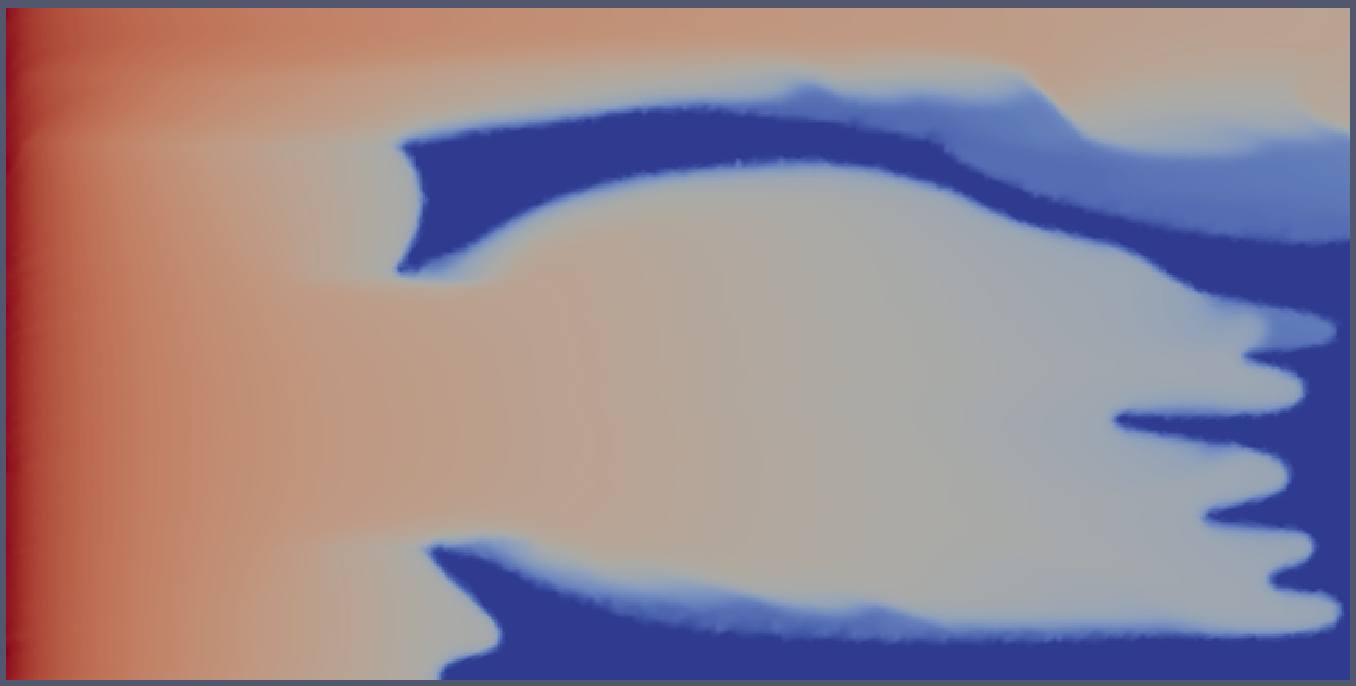
\includegraphics[width=.65\textwidth]{./Pics1/mr10_5regions_fixed/5regions_fixed_1500.pdf} 
}
\vspace{0.0cm}
\hbox{\hspace{6.5cm} (a) flow at t=1500 (fixed mesh)   
}
\vspace{0.25cm}
\hbox{\hspace{3.5cm}
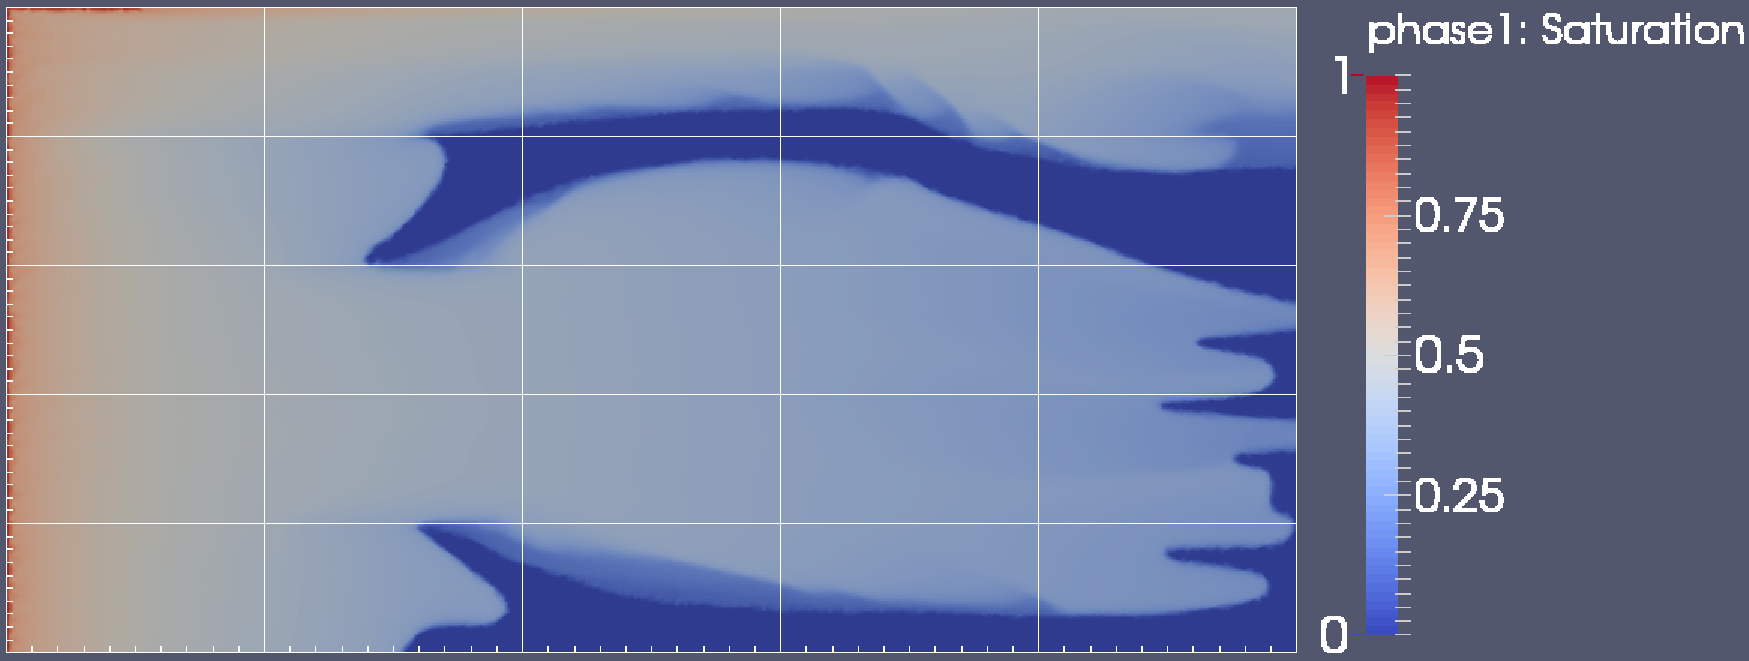
\includegraphics[width=.9\textwidth]{./Pics1/mr10_5regions_adapt/5regions_adapt_1500_1.pdf}
}
\vspace{0.0cm}
\hbox{\hspace{6.5cm} (b) flow at t=1500 (adaptive mesh)     
}
}     
\caption{At $t=0.75 sec$ ($t=1500$, timestemp) the initial cross flow is now fully developed and has travel all the way towards the outlet (right-hand side). and the finger below start forming a front that is also travelling towards the left-hand side.}
\label{fig:2testcase_c}
\end{figure}
\end{landscape}
\clearpage



%%%%
%%%%  FIGURE
%%%%
\begin{landscape}
\begin{figure}[ht] 
\vbox{
\hbox{\hspace{3.5cm}
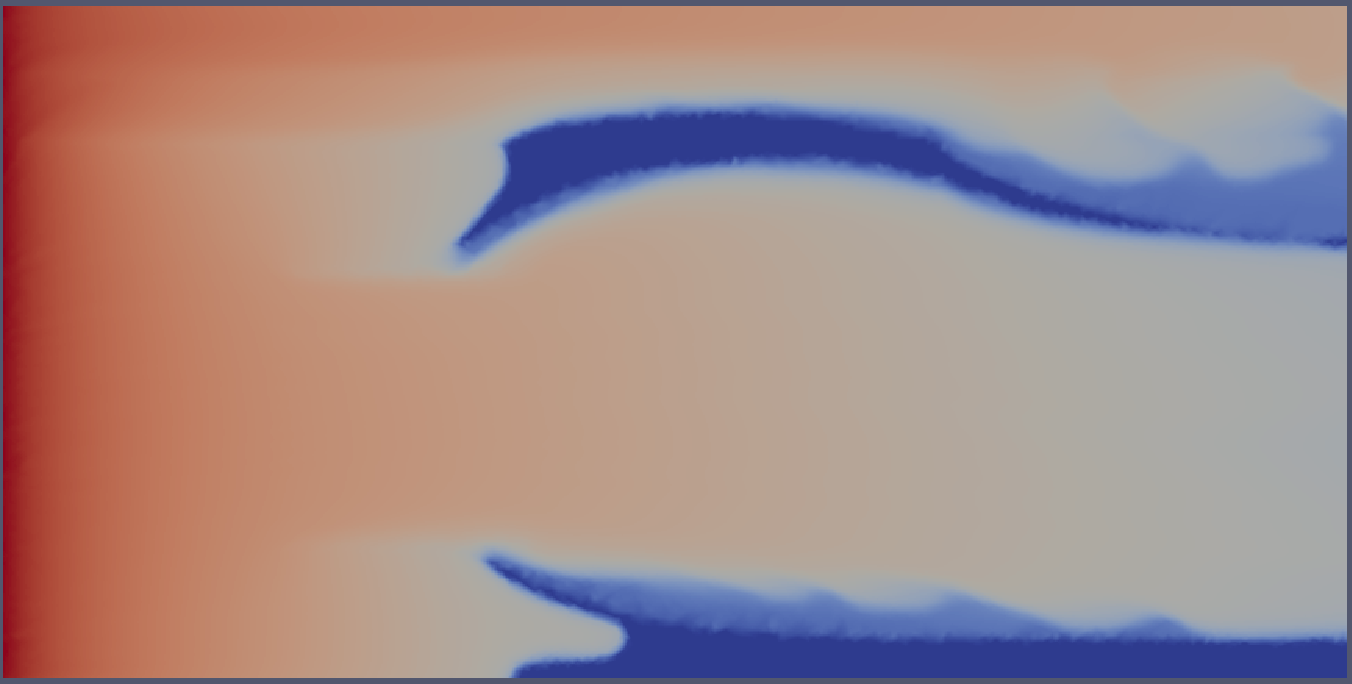
\includegraphics[width=.65\textwidth]{./Pics1/mr10_5regions_fixed/5regions_fixed_2000.pdf} 
}
\vspace{0.0cm}
\hbox{\hspace{6.5cm} (a) flow at t=end (fixed mesh)   
}
\vspace{0.25cm}
\hbox{\hspace{3.5cm}
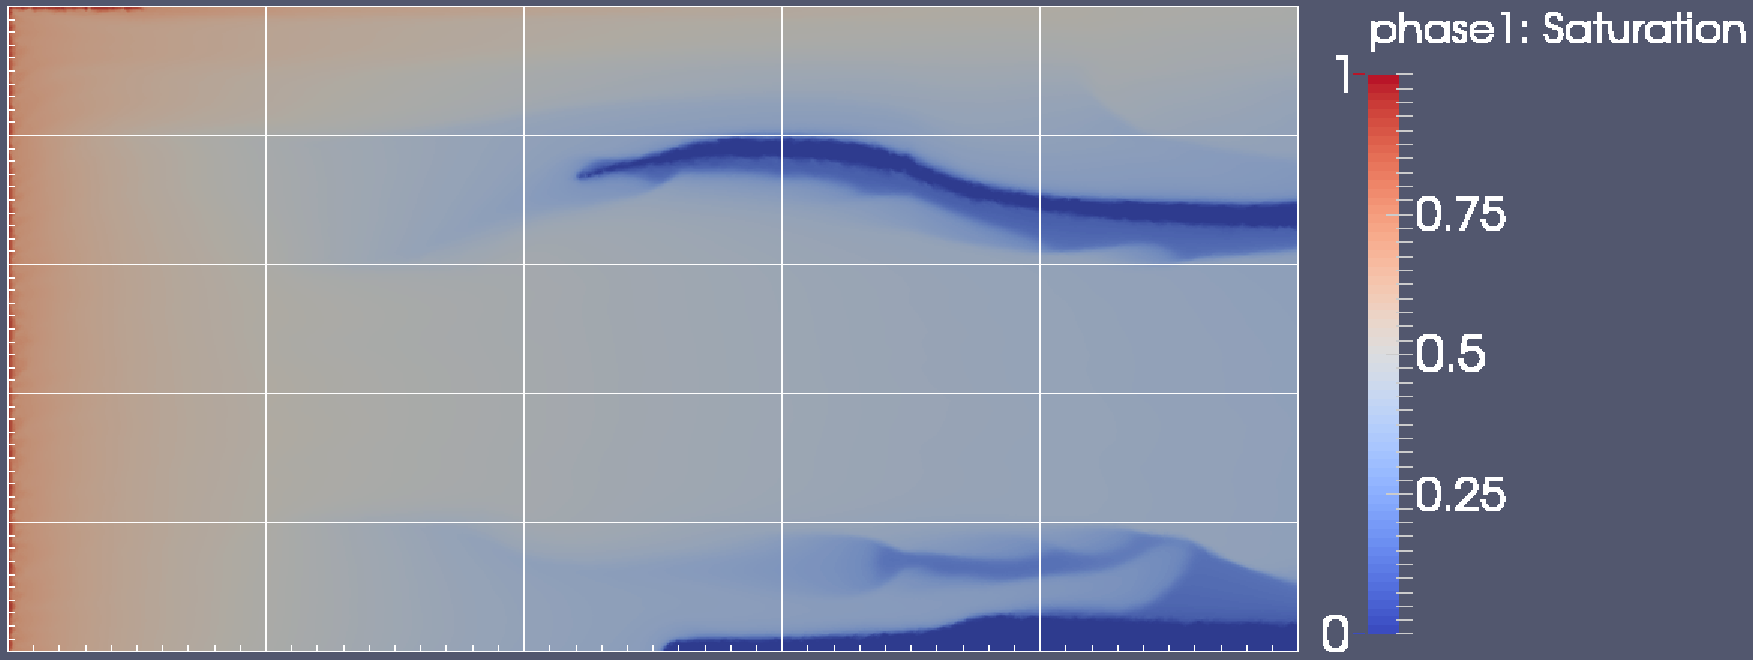
\includegraphics[width=.9\textwidth]{./Pics1/mr10_5regions_adapt/5regions_adapt_3000_1.pdf}
}
\vspace{0.0cm}
\hbox{\hspace{6.5cm} (b) flow at t=end (adaptive mesh)     
}
}     
\caption{Using the $P_{1}DGP_{2}$ element type for VR=$10$ under the same time steps, we compared the impact of fixed and adaptive mesh for the same timeframe. The end of simulation happens at $time=5 sec$ and for the timestemp $t=9999$ while the number of elements in both simulations was approximately $4700$. When adaptive mesh is introduce there is better repersentation of the fluid instabilities as these are developed on time.}
\label{fig:2testcase_d}
\end{figure}
\end{landscape}
\clearpage



%%%%
%%%%  FIGURE
%%%%
\begin{landscape}
\begin{figure}[ht] 
\vbox{
\hbox{\hspace{3.5cm}
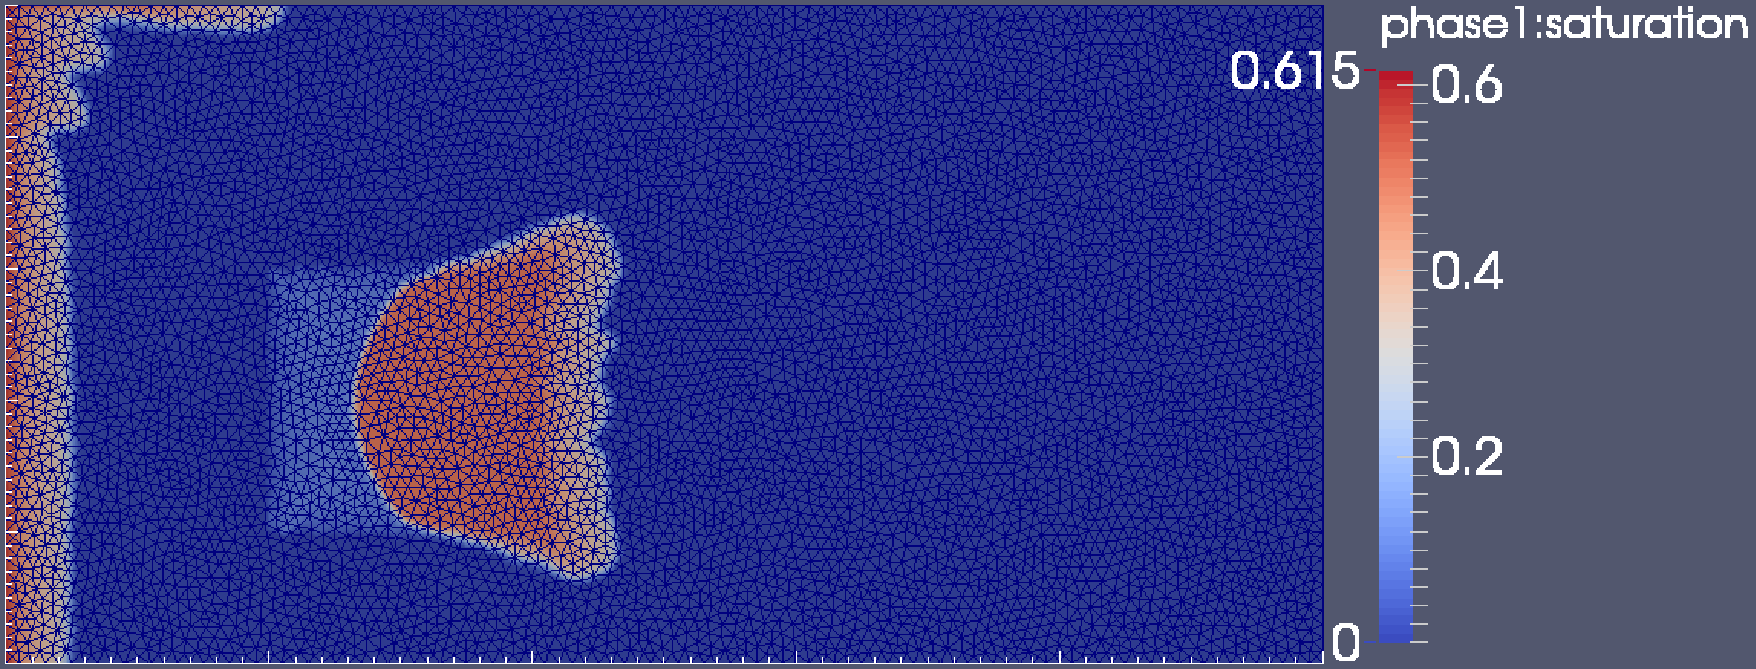
\includegraphics[width=.9\textwidth]{./Pics1/mr10_5regions_fixed_dinlet/5regions_dinlet_fixed_100_1.pdf}
}
\vspace{0.0cm}
\hbox{\hspace{6.5cm} (a) double inlet - fixed mesh   
}
\hbox{\hspace{3.5cm}
  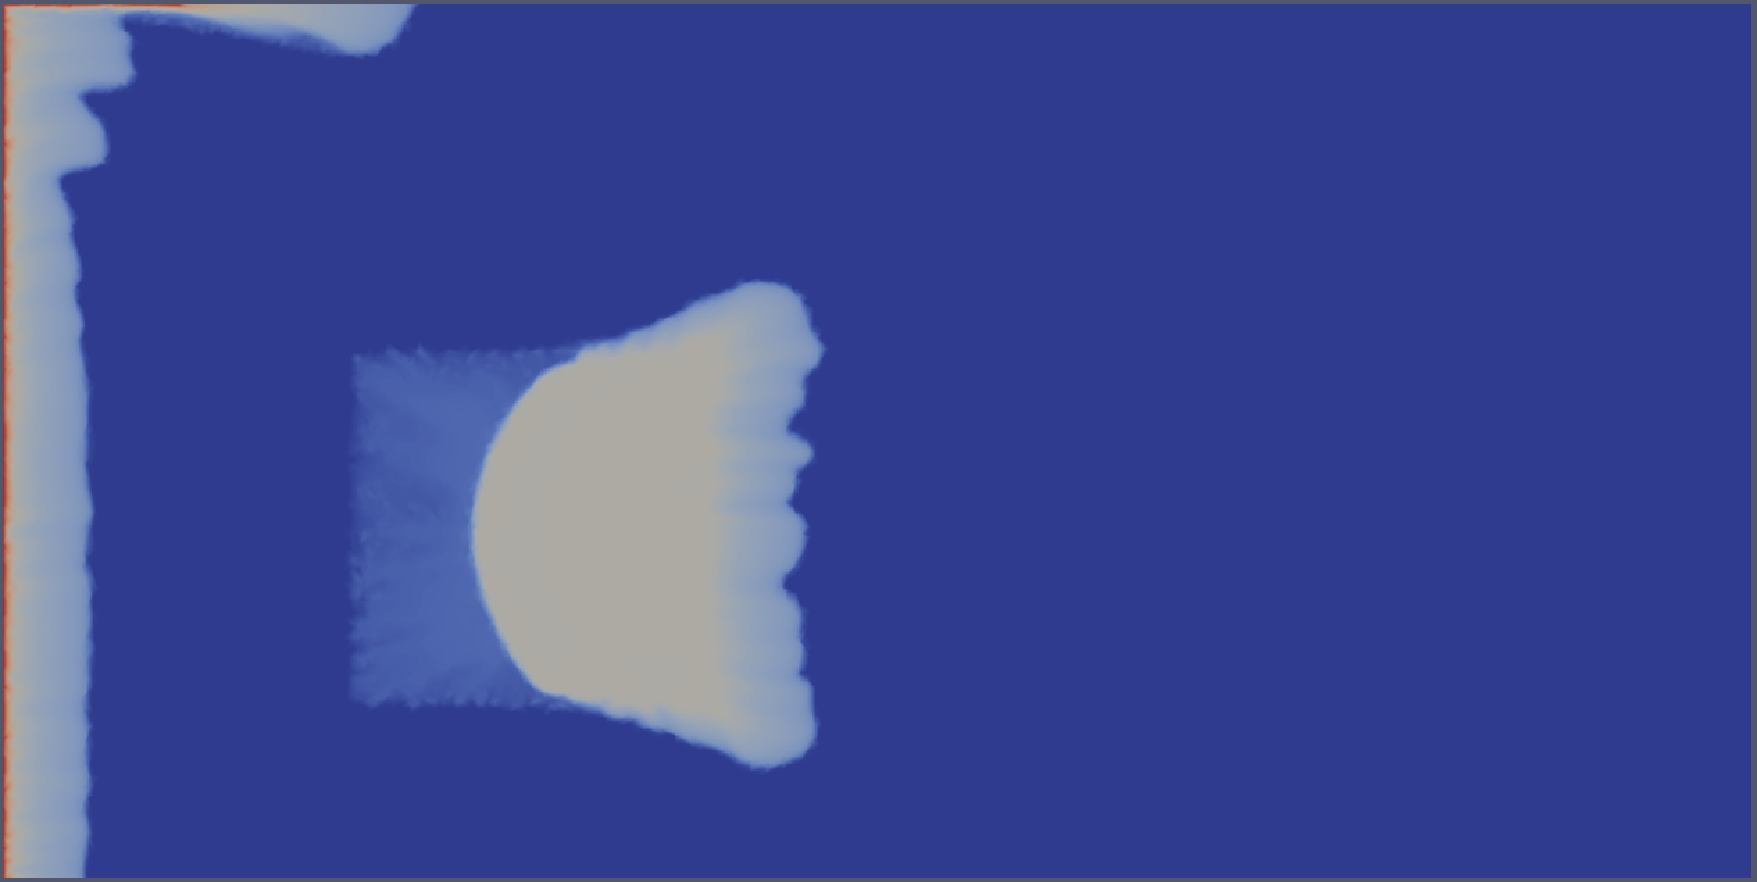
\includegraphics[width=.67\textwidth]{./Pics1/mr10_5regions_adapt_dinlet/5regions_dinlet_adapt_start.pdf}
}
\vspace{0.0cm}
\hbox{\hspace{6.5cm} (b) double inlet adaptive mesh   
}
}     
\caption{Comparing test-cases of fixed and adaptive mesh while a second region/inlet is introduced. For $t=0.101$s, using the $P_{1}DGP_{2}$ element type for MR=$10$ under the same time steps. For this simulation there are $13226$ elements for the fixed messh and $43716$ for the adaptive.}
\label{fig:3testcase_a}
\end{figure}
\end{landscape}
\clearpage

%%%%
%%%%  FIGURE
%%%%
\begin{figure}[ht] 
\vbox{
\hbox{\hspace{3.5cm}
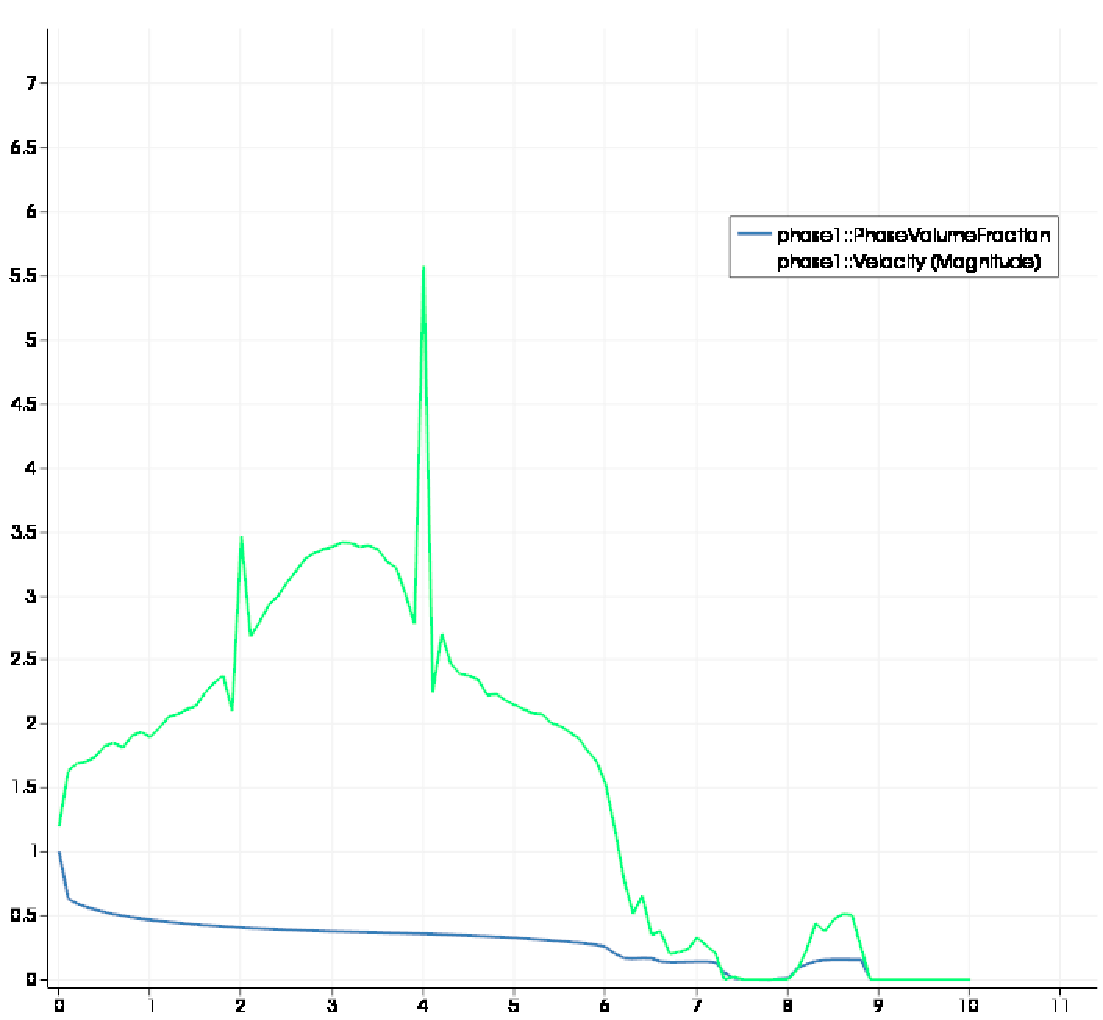
\includegraphics[width=.5\textwidth]{./Pics1/mr10_5regions_adapt/5regions_adapt_vel_magn.pdf} 
}
\vspace{0.0cm}
\hbox{\hspace{5.0cm} (a) single inlet velocity magnitude   
}
\hbox{\hspace{3.5cm}
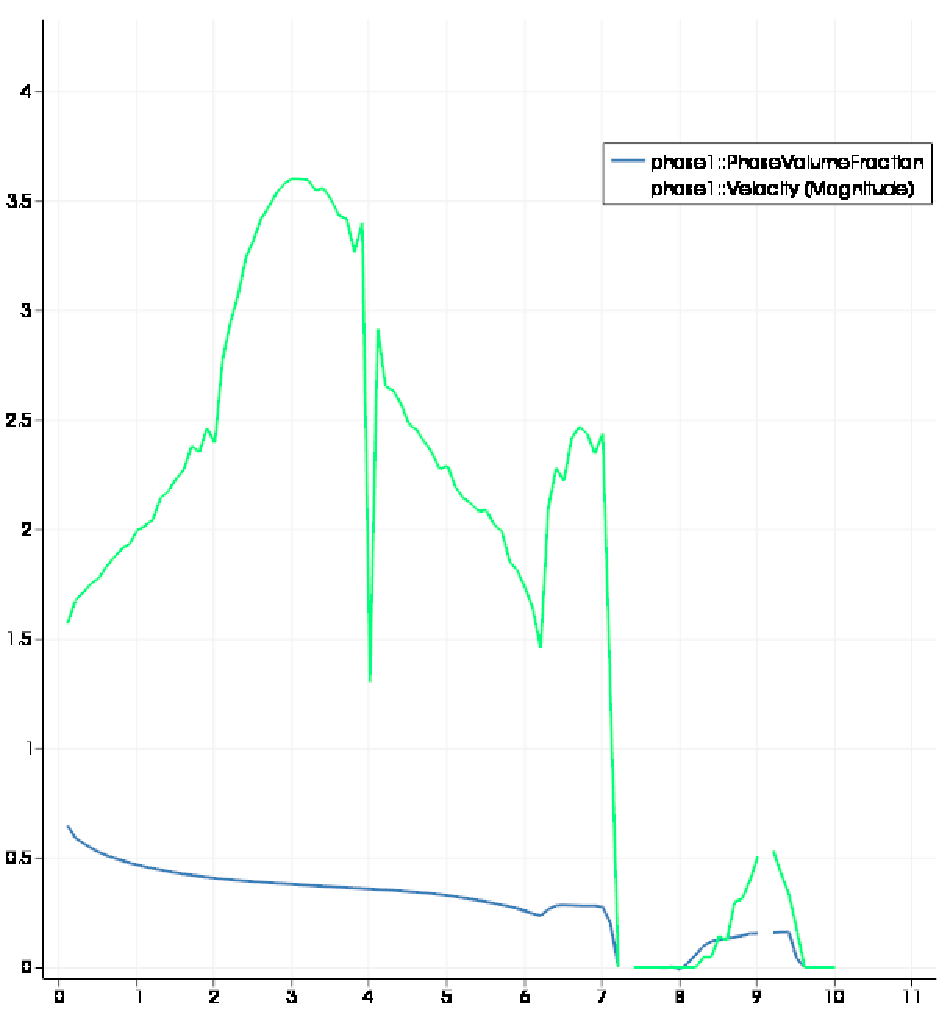
\includegraphics[width=.5\textwidth]{./Pics1/mr10_5regions_adapt_dinlet/5regions_dinlet_adapt_vel_magn.pdf}
}
\vspace{0.0cm}
\hbox{\hspace{5.0cm} (b) double inlet velocity magnitude   
}
}     
\caption{For the same time step, t=1000, these plots describe the velocity magnitudes of the phase $1$ (injected fluid) under the same boundary and initiall conditions. From top to bottom,these graphs describe the velocity magnitude %for fixed mesh is plotted(top), the velocity magnitude 
for adaptive mesh-single inlet (top) and the velocity magnitude for adaptive mesh with double inlet (bottom) as these are also presented in fig.\ref{fig:3testcase_a}. The main difference between the upper and lower plot %is not just the ability to capture in greater detail, the fluid instabilities as they happenduring the finger development and their velocity patterns. While there 
is the impact of the second injection interval as this can be seen from the slope and the rate that the velocity magnitude is changing.}
\label{fig:vel_magn}
\end{figure}

%%%%
%%%%  FIGURE
%%%%
\begin{landscape}
\begin{figure}[ht] 
\vbox{
\hbox{\hspace{3.5cm}
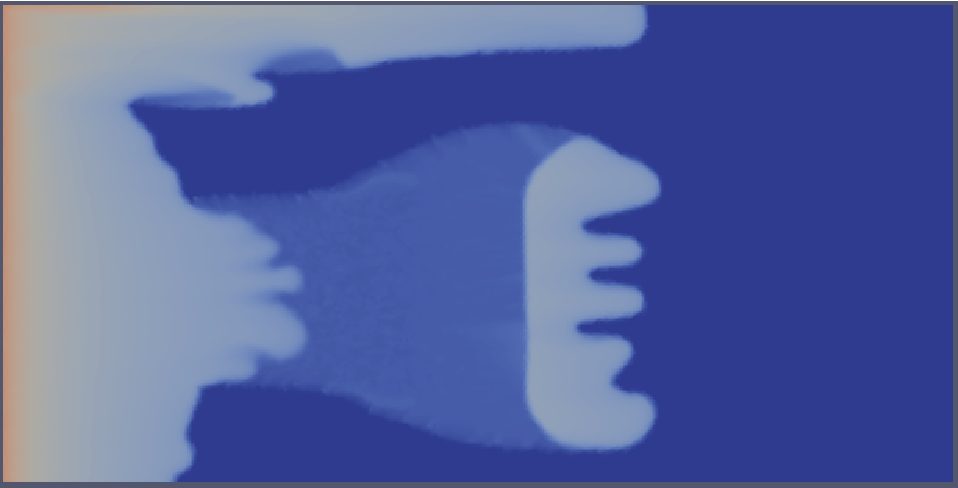
\includegraphics[width=.65\textwidth]{./Pics1/5reg_dinlet_fixed_500.pdf} 
}
\vspace{0.0cm}
\hbox{\hspace{6.5cm} (a) double inlet - fixed mesh   
}
\hbox{\hspace{3.5cm}
\includegraphics[width=.9\textwidth]{./Pics1/5reg_dinlet_adapt_500_1.pdf}
}
\vspace{0.0cm}
\hbox{\hspace{6.5cm} (b) double inlet adaptive mesh   
}
}     
\caption{For $t=5$s there is a comparison between fixed mesh(a) and adaptive mesh(b).}
\label{fig:3testcase_b}
\end{figure}
\end{landscape}
\clearpage

%%%%
%%%%  FIGURE
%%%%
\begin{landscape}
\begin{figure}[ht] 
\vbox{
\hbox{\hspace{3.5cm}
\includegraphics[width=.65\textwidth]{./Pics1/5reg_dinlet_fixed_1500.pdf} 
}
\vspace{0.0cm}
\hbox{\hspace{6.5cm} (a) double inlet - fixed mesh   
}
\hbox{\hspace{3.5cm}
\includegraphics[width=.9\textwidth]{./Pics1/5reg_dinlet_adapt_1500_1.pdf}
}
\vspace{0.0cm}
\hbox{\hspace{6.5cm} (b) double inlet adaptive mesh   
}
}     
\caption{For $t=7.5$s this is a comparison between fixed mesh(a) and adaptive mesh(b).}
\label{fig:3testcase_c}
\end{figure}
\end{landscape}
\clearpage

%%%%
%%%%  FIGURE
%%%%
\begin{landscape}
\begin{figure}[ht] 
\vbox{
\hbox{\hspace{3.5cm}
\includegraphics[width=.65\textwidth]{./Pics1/5reg_dinlet_fixed_end.pdf} 
}
\vspace{0.0cm}
\hbox{\hspace{6.5cm} (a) double inlet - fixed mesh   
}
\hbox{\hspace{3.5cm}
\includegraphics[width=.9\textwidth]{./Pics1/5reg_dinlet_adapt_end_1.pdf}
}
\vspace{0.0cm}
\hbox{\hspace{6.5cm} (b) double inlet adaptive mesh   
}
}     
\caption{This is a comparison between fixed mesh(a) and adaptive mesh(b) at the end of the simulation. For the fixed mesh at this point the maximum number of point is $13226$ while for the adaptive mesh is $7582$ and most of them are located where is needed in the domain.}
\label{fig:3testcase_d}
\end{figure}
\end{landscape}
\clearpage

%%%%
%%%%  FIGURE
%%%%
\begin{landscape}
\begin{figure}[ht] 
\vbox{
\hbox{\hspace{3.5cm}
\includegraphics[width=.8\textwidth]{./Pics1/mr100_fixed/mr100_fixed_500.pdf} 
}
\vspace{0.0cm}
\hbox{\hspace{4.0cm} (a) fixed and unstructured mesh for MR = 100 (start)   
}
\hbox{\hspace{3.5cm}
\includegraphics[width=.8\textwidth]{./Pics1/mr100_fixed/mr100_fixed_1500.pdf}
}
\vspace{0.0cm}
\hbox{\hspace{3.75cm} (b) fixed and unstructured mesh for MR = 100 (t = 1500)   
}
}     
\caption{For the case of VR=$100$ from top to bottom, the number of elements is $4680$ and fixed and unstructured mesh for the same time steps, t=$0.25$ or t=500(a), t=$0.75$ or t=1500(b). }
\label{fig:4testcase_a}
\end{figure}
\end{landscape}
\clearpage

%%%%
%%%%  FIGURE
%%%%
\begin{landscape}
\begin{figure}[ht] 
\vbox{
\hbox{\hspace{3.5cm}
\includegraphics[width=.8\textwidth]{./Pics1/mr100_fixed/mr100_fixed_3000.pdf} 
}
\vspace{0.0cm}
\hbox{\hspace{3.75cm} (c) fixed and unstructured mesh for MR = 100    
}
\hbox{\hspace{3.5cm}
\includegraphics[width=.8\textwidth]{./Pics1/mr100_fixed/mr100_fixed_end.pdf}
}
\vspace{0.0cm}
\hbox{\hspace{7.cm} (d) end of simulations     
}
}     
\caption{screenshot (c) is for t=$1.5$ sec or t=$3000$ and screenshot (d) is for t=$3.175$ sec, at the end of the simulations. }
\label{fig:4testcase_b}
\end{figure}
\end{landscape}
\clearpage



%

%%%
%%%  FIGURE 
%%%
\begin{figure}[h]
\begin{center}
\includegraphics[width=1.\textwidth]{diagrams/bl-exact-meth-upwind.eps}
\end{center}
\caption{Buckley--Leverett test-cases: Saturation solutions for the continuous upwind method for different 1D P$_{1}$DG-P$_{2}$ mesh  resolutions and comparison against standard analytical solution.
\label{bl-exact-meth-upwind}}
\end{figure}

%%%
%%%
%%%  FIGURE 
%%%
\begin{figure}[h]
  %\begin{center}
\vbox{\hbox{\hspace{2.5cm}
    \includegraphics[width=0.62\textwidth]{diagrams/BL_1d_P0DGP1_convergence.eps}}
\vspace{-.0cm}\hbox{\hspace{2.5cm}
    \includegraphics[width=0.62\textwidth]{diagrams/BL_1d_P1DGP2_convergence.eps}}
\vspace{-.0cm}\hbox{\hspace{2.5cm}
    \includegraphics[width=0.62\textwidth]{diagrams/BL_1d_P2DGP3_convergence.eps}}}
   % \includegraphics[width=0.45\textwidth]{BL_2d_P1DGP2_convergence}
    \caption{Buckley--Leverett test-cases: Saturation profiles for a number of element-pairs and numerical resolutions in 1D -- P$_{0}$DG-P$_{1}$ (top), P$_{1}$DG-P$_{2}$ and P$_{2}$DG-P$_{3}$ (bottom).\label{fig:BL_profiles}}
  %\end{center}
\end{figure}

%%%
%%%  FIGURE 
%%%
\begin{figure}[h]
\vbox{\hbox{\hspace{1.cm}
    \includegraphics[width=0.8\textwidth]{diagrams/L1_convergence_rate.eps}}
\vspace{.0cm}\hbox{\hspace{1.cm}
    \includegraphics[width=0.8\textwidth]{diagrams/L2_convergence_rate.eps}}}
    \caption{Buckley--Leverett test-cases: L1 (top) and L2 (bottom) error convergence rates for a number of element pairs. \label{fig:BL_converg-rates}}
\end{figure}

%%%
%%%  FIGURE 
%%%
\begin{figure}[h]
\begin{center}
\includegraphics[width=1.\textwidth]{diagrams/bl-upwind-v-up-and-down.eps}
\end{center}
\caption{Buckley--Leverett test-cases: Comparison of the optimal upwind formulation when using upwinding (OU) and coupled upwind/downwind (OU-D). The finite element interpolation of the saturation field $\left(S_{1}\right)$ is shown at different mesh resolutions. Downwind seems to detract from the accuracy of the solution. \label{bl-upwind-v-up-and-down}}
\end{figure}

%%%
%%%  FIGURE 
%%%
\begin{figure}[h]
\vbox{
\begin{center}
\includegraphics[width=1.\textwidth]{diagrams/bl-exact-meth-cv-0-8-ele50.eps}
\end{center}
\vspace{0.cm}}
\caption{Buckley--Leverett test-cases: Comparison of control volume
  solutions using 80$\%$ upwinding and with optimal upwinding and
  using 50 continuous P$_{1}$DG-P$_{2}$
  elements. \label{bl-exact-meth-cv-0-8-ele50}}
\end{figure}

%%%
%%%  FIGURE 
%%%
\begin{figure}[h]
\begin{center}
\includegraphics[width=1.\textwidth]{diagrams/bl-dg-2eles.eps}
\end{center}
\caption{Buckley--Leverett test-cases: Two element solution using the
  discontinuous formulation. Saturation field from both CV solution
  and FEM interpolation are shown.  \label{bl-dg-2eles}}
\end{figure}

%%%
%%%  FIGURE 
%%%
\begin{figure}[h]
\vbox{
\hbox{\hspace{.3cm}\includegraphics[width=.9\textwidth]{diagrams/bl-dg-4-10-20.eps}}
\vspace{-0.cm}
\hbox{\hspace{.3cm}\includegraphics[width=.9\textwidth]{diagrams/bl-dg-cent-4-10-20.eps}}}
\caption{Buckley--Leverett test-cases: Saturation field obtained from
  the discontinuous and continuous formulation with different mesh
  resolutions. Solutions with (top) and without (bottom) upwinding
  scheme. Notice that oscillations are suppressed with the upwinding
  scheme.\label{bl-dg-cent-4-10-20}}
\end{figure}


%%%
%%%  FIGURE 
%%%
\begin{figure}[h]
\vbox{
\hbox{\hspace{.3cm}\includegraphics[width=.9\textwidth]{diagrams/bl-dg-4-10-vers-cty.eps}}
\vspace{-0.cm}
\hbox{\hspace{.3cm}\includegraphics[width=.9\textwidth]{diagrams/bl-dg-p1-2-4-5-10-20-40.eps}}}
\caption{Buckley--Leverett test-cases: Saturation field obtained from
  (top) continuous and discontinuous (between elements) formulations
  (solution with 50 elements may be considered as a converged
  result). Solution obtained (bottom) from linear pressure (P1)
  formulation with different mesh resolution with comparison against
  P2-pressure formulation (continuous). \label{bl-dg-4-10-vers-cty}}
\end{figure}


%%%
%%%  FIGURE 
%%%
\begin{figure}[H]
\vbox{
\begin{center}
\includegraphics[width=17.5cm,height=12.5cm]{diagrams/bl-dg-4-10-vers-cty}
\end{center}
\vspace{0.cm}}
\caption{Gas saturations shown comparing the accuracy of the
  discontinuous between elements and continuous formulation. The 50
  element continuous solution may be viewed as a converged result.  }
\label{bl-dg-4-10-vers-cty}
\end{figure}

\begin{comment}
%%%
%%%  FIGURE 
%%%
\begin{figure}[h]
\vbox{
\hbox{\hspace{.2cm}
    \includegraphics[width=1.\textwidth]{diagrams/map_2d.png}}
\vspace{1.cm}
\hbox{\hspace{0.2cm}
    \includegraphics[width=1.\textwidth]{./diagrams/map_3d.png}}}
    \caption{Buckley-Leverett test-cases: phase 1 saturation surface maps for a 2- (770 triangles) and 3-D (1207 tetrahedra) simulations (\PN[1]{2} unstructured mesh grids) at time $t=0.5$. \label{fig:maps2d_3d}}
\end{figure}


%%%  FIGURE 
%%%
\begin{figure}[h]
\vbox{\hbox{\hspace{.3cm}
    \includegraphics[width=0.9\textwidth]{diagrams/BL_2d_P1DGP2_convergence.eps}}
\vspace{-.0cm}\hbox{\hspace{.3cm}
    \includegraphics[width=0.9\textwidth]{./diagrams/simulations_2d_3d.eps}}}
    \caption{Buckley-Leverett test-cases: 2- and 3-D phase 1 saturation profiles with \PN[1]{2} elements. Sensitivity analysis for (top) grid resolution using structured \PN[1]{2} mesh, and (bottom) mesh type.\label{fig:BL_2d_profiles}}
\end{figure}

\end{comment}
 

\end{document}
%% End of tex file.


